\documentclass[12pt,letterpaper, oneside]{book}
%% THESIS STARTER KIT
% use these files to see if you can compile using your program of choice
\usepackage{enpThesis}
\graphicspath{{Figures/}}
\usepackage{SF298/sf298}
\usepackage{cite}	
\usepackage{url}
\usepackage{subfigure}
\usepackage{multirow}
\usepackage{rotating}
\usepackage{caption}
%\usepackage{notoccite}% PREVENTS CITES IN CAPTIONS FROM MISNUMBERING YOUR REFERENCES 

  

% Experimental additions to fix formatting errors -----------------------------------------
%\geometry{top=1in, bottom=1.25in, left=1.25in, right=1.25in}
%\setlength{\intextsep}{0.5in}
%\setlength{\floatsep}{0.5in}
%\setlength{\belowcaptionskip}{0.15in}
%\setlength{\abovecaptionskip}{0.15in}
% -------------------------------------------------------------------------------------------------------

% DATA OF AUTHOR AND THESIS:

\prospectus

\author{Nicholas J. Quartemont}
\rank{First Lieutenant, USAF}
\title{Application of Spectral Shaping for Simulating Nuclear Weapon 
Environments}
% Need to check - should title be in caps case?  All examples I have point to yes.

\flytitle{APPLICATION OF SPECTRAL SHAPING FOR SIMULATING NUCLEAR WEAPON ENVIRONMENTS}

\docdesignator{AFIT-ENP-MS-19-M}         


\distribution{NOT YET DISTRIBUTION STATEMENT A\\[-10pt]
\MakeUppercase{NOT YET Approved for Public Release; NOT YET distribution 
unlimited.}
} 

\disclaimer{The views expressed in this thesis are those of the author and 
do not reflect the official policy or position of the United States Air Force, 
Department of Defense, or the United States Government.  This material is 
declared a work of the U.S. Government and is not subject to copyright 
protection in the United States.}

\previousdegrees{BS}

\acdegree{Master of Science in Nuclear Engineering}

\graduationdate{March 2019}

\address{2950 Hobson Way\\ Air Force Institute of Technology \\ Wright-Patterson AFB, OH 45433}

\department{Department of Engineering Physics}


\committee{{Capt James E. Bevins (Advisor)}, {Dr. James C. Petrosky (Member)},
	{Dr. Abigail A. Bickley  (Member)}, {Lt Col Michael B. Shattan (Member)}}


% define custom commands
\newcommand{\regmark}{\raisebox{5pt}{\tiny \circledR}\xspace}
\newcommand{\matlab}{\textsc{Matlab}\regmark}
\newcommand{\trademark}{\raisebox{5pt}{\tiny TM}\xspace}
\newcommand{\mca}{\texttt{Mathematica}\regmark}
\newcommand{\Latex}{\LaTeX\xspace}

% Create a new theorem style called a Corollary.
% If you don't have any, then just comment this out.
%\theoremstyle{plain} % Default
\newtheorem{cor}{Corollary}[chapter]

%Custom Commands for Student

\newcommand{\primerAddress}{{L:$\backslash$Courses$\backslash$PHYS$\backslash$LaTeX}\xspace}

%% myFigures.tex
% A common file to store all figure definitions
%
% In preparing your thesis, one of the first things you should do is
% organize your figures.  Then, one of the last things you'll do is
% reorder your figures so they display where you want them to in the
% text.  Organizing figure definitions in a common files helps:
%
%   1. Write new figures using earlier examples.
%
%   2.  Isolate code and minimize the risk of introducing bugs in the
%   final editing process.  Trust me, moving around just one line of
%   code is easier.
%
%   3.  Reuse figures in other papers.  <=== the best reason!
%
% Note command names can not include numbers and special characters.
%
% To make the file more searchable, use naming conventions that map
% the graphics filename labSetup.jpg to the command name \figlabSetup to the
% figure label fig:labSetup.
% 

\newcommand{\figMyFirstLaTeX}{\begin{figure}[tbp]
 \begin{center}
    
\includegraphics[width=6in]{myFirstLaTeXCursor}
     \caption[\LaTeX\ a very simple document]{Compile a very simple document.}
     \label{fig:MyFirstLaTeX}
 \end{center}
 \vspace{-0.2 in}
\end{figure}
}


\newcommand{\figafitStyle}{\begin{figure}[tbp]
 \begin{center}
    
\includegraphics[width=6in]{myFirstLaTeXafit}
     \caption{Recompile using afitThesis.sty, the AFIT
     thesis style file.}
     \label{fig:afitStyle}
 \end{center}
\end{figure}
}


\newcommand{\figtitlePage}{\begin{figure}[tbp]
 \begin{center}
    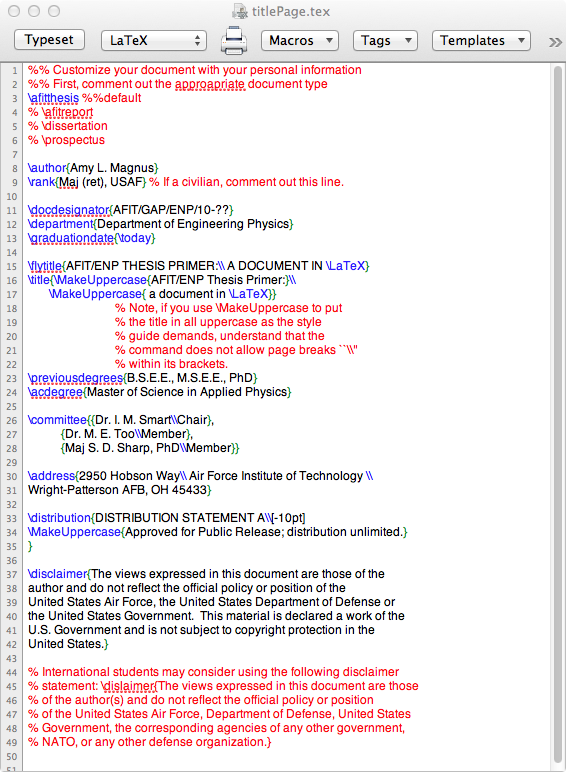
\includegraphics[width=6in]{titlePage}
     \caption{Enter student data in titlePage.tex to customize the
     document's first pages.}
     \label{fig:titlePage}
 \end{center}
\end{figure}
}

\newcommand{\figmyFlypage}{\begin{figure}[tbp]
 \begin{center}
    
\includegraphics[width=6in]{myFlypage}
     \caption{Here we have compiled the first four page of a thesis.}
     \label{fig:myFlypage}
 \end{center}
\end{figure}
}

\newcommand{\figmyFirstAbstract}{\begin{figure}[tbp]
 \begin{center}
    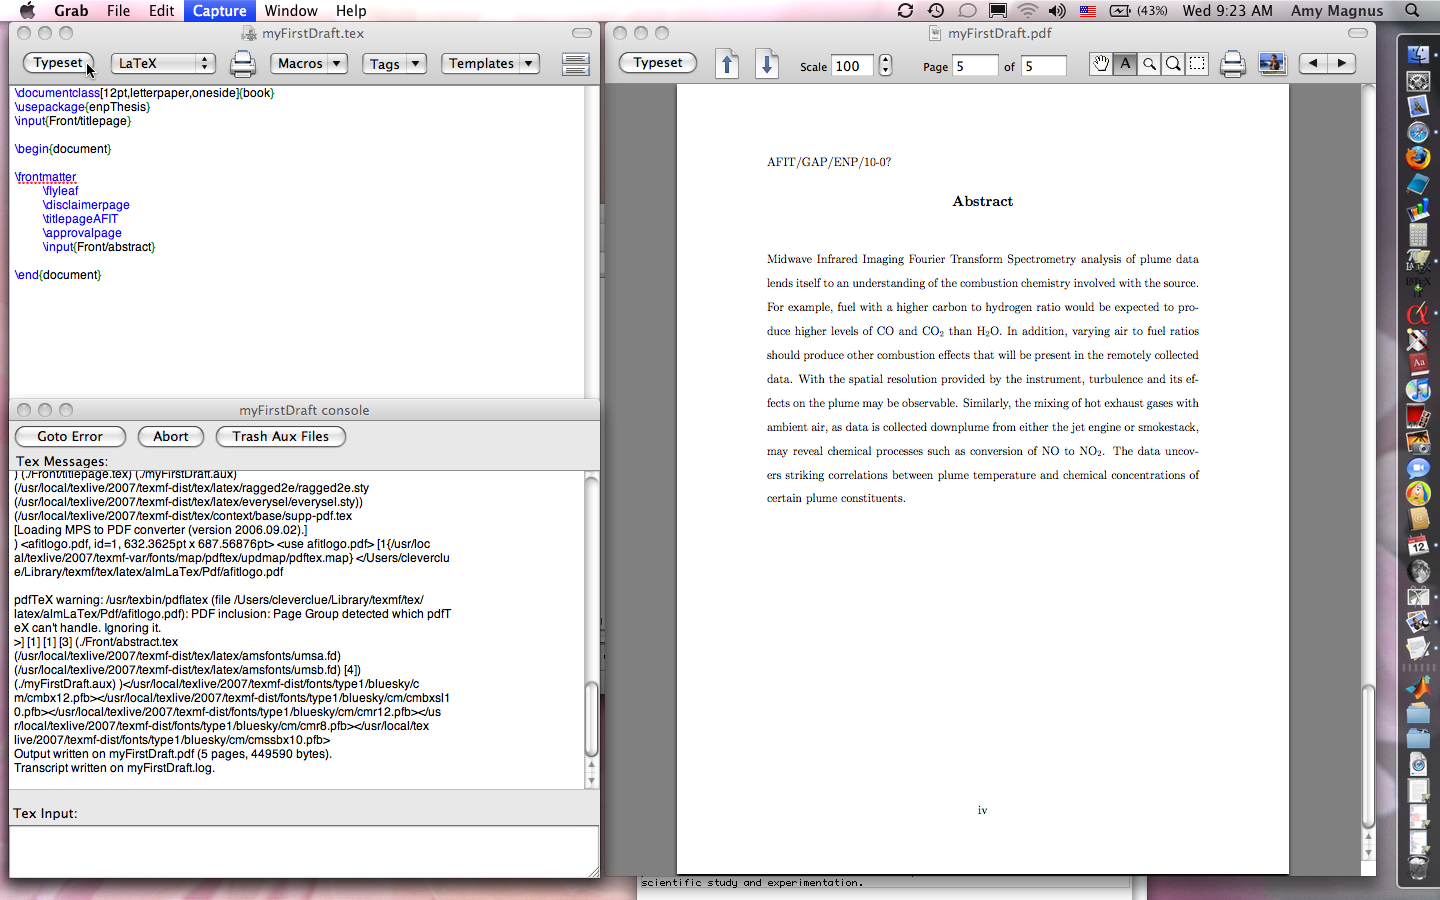
\includegraphics[width=6in]{myFirstAbstract}
     \caption{Add an abstract to the front matter of your thesis.}
     \label{fig:myFirstAbstract}
 \end{center}
\end{figure}
}

\newcommand{\figmyFigures}{\begin{figure}[tbp]
 \begin{center}
    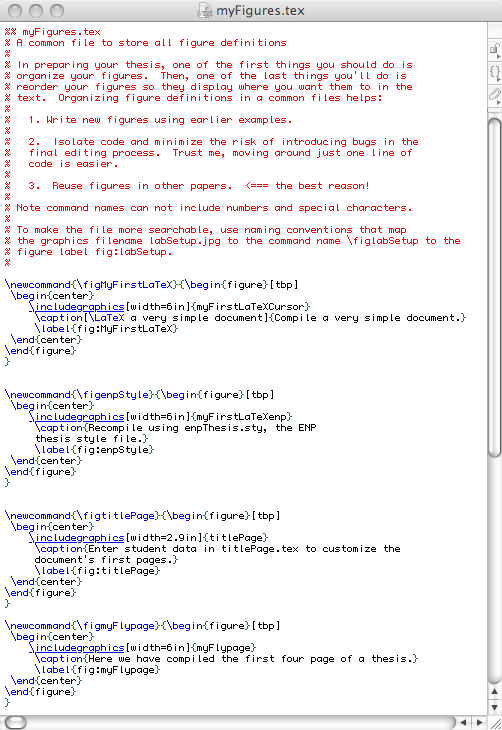
\includegraphics[width=5in]{myFigures}
     \caption{Consider defining all your figures in one file.}
     \label{fig:myFigures}
 \end{center}
\end{figure}
}


\newcommand{\figmyFirstFigures}{\begin{figure}[tbp]
 \begin{center}
    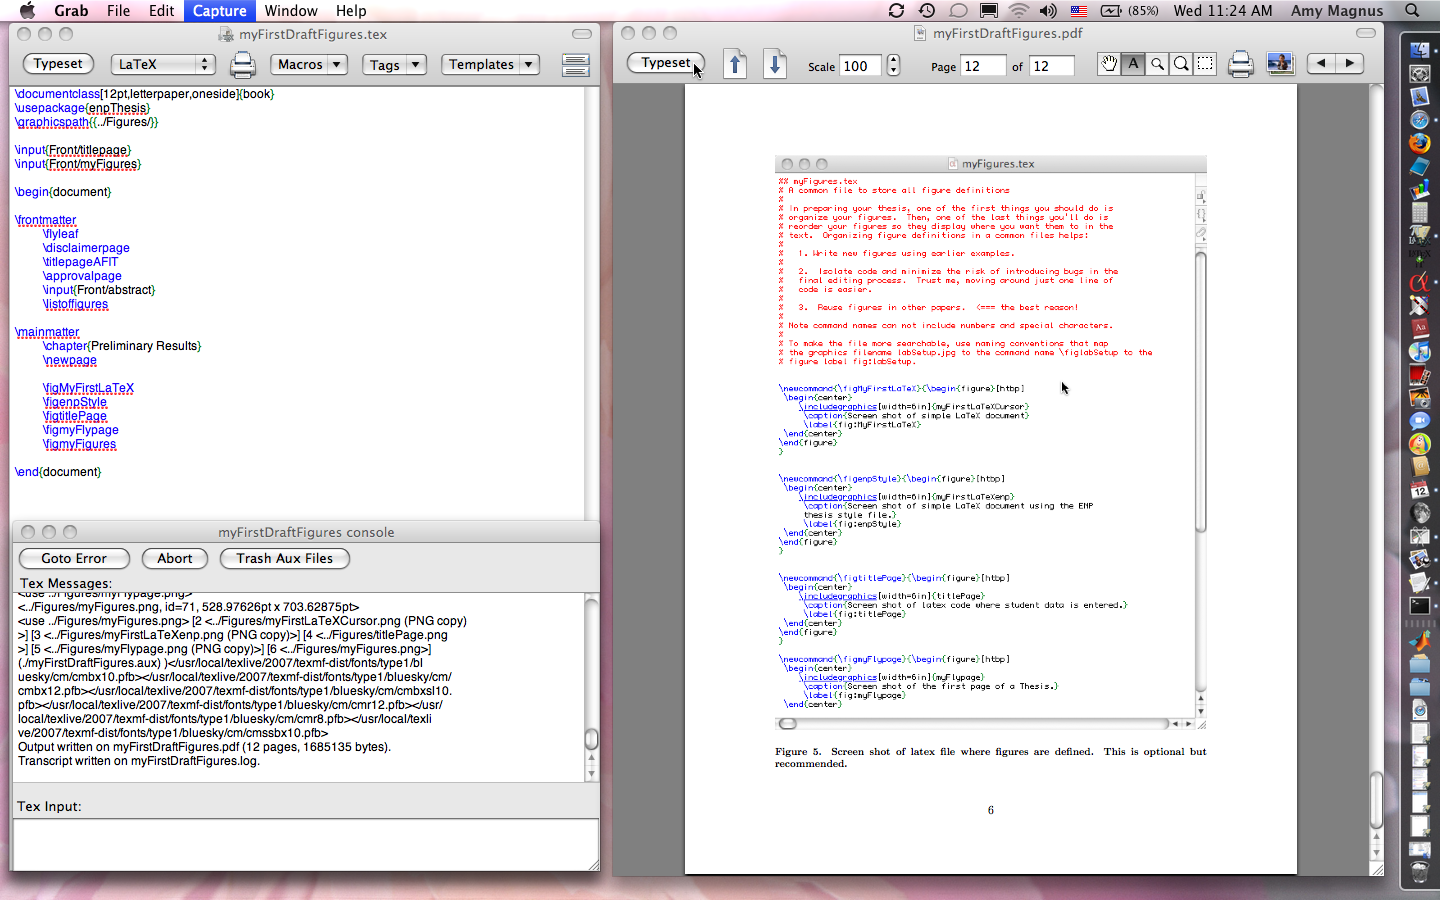
\includegraphics[width=6in]{myFirstFigures}
     \caption{Add figures in the main matter of your document; fill in
     the document around your graphics.}
     \label{fig:myFirstFigures}
 \end{center}
\end{figure}
}

\newcommand{\figmyFirstBibTeX}{\begin{figure}[tbp]
 \begin{center}
    \includegraphics[width=6in]{myFirstBibTeX}
     \caption{Add your bibliography.}
     \label{fig:myFirstBibTeX}
 \end{center}
\end{figure}
}







\newcommand{\tabRadiometricQuantities}{
\begin{table}[htbp]
  \centering
  \caption{Radiometric Quantities in SI units.}\label{tab:RadiometricQuantities}
\begin{tabular}{|c|c|c|c|}
  \hline
  Symbol & Name & Units & Definition \\
  \hline
  $A$ & area & cm$^2$ & projected area of source \\
  $R$ & length & cm & distance between source and \\
  &  &  & collection optic \\
  $\theta$ & linear angle & rad & angle between source and  \\
  &  &  & collection optic \\
  $\Omega$ & solid angle & sr & $d\Omega = \frac{dA}{R^2}$ \\
  $\phi$ & flux & W & radiant energy reaching collection optic \\
   &  &  & per unit time \\
  $L$ & radiance & $\frac{W}{cm^2 sr}$ & $L = \frac{\partial^2 \phi}{\partial A \cos \theta \partial \Omega}$ \\
  $I$ & intensity & $\frac{W}{sr}$ & $I = \frac{\partial \phi}{\partial \Omega} = \int_A L \cos \theta dA$ \\
  $F$ & irradiance & $\frac{W}{cm^2}$ & $F = \frac{\partial \phi}{\partial A_d}$ $A_d = $ area of collection optic \\
  $B_{\bar{\nu}}$ & Planck distribution & $\frac{W}{cm^2 sr cm^{-1}}$ & $B_{\bar{\nu}} d\bar{\nu} = \frac{2 h c^2 {\bar{\nu}}^3}{\exp(\frac{h c \bar{\nu}}{k_B T}) - 1} d\bar{\nu}$ \\
  \hline
\end{tabular}
\end{table}
}


\newcommand{\tabFullSpectrumInitialFit}{
\begin{table}
\caption{Initial analysis with full spectrum fit of r, T, H$_2$0,
CO$_2$, CO fit parameters} \label{tbl:FullSpectrumInitialFit}
\begin{center}
\begin{tabular}{|c|c|c|c|c|c|}\hline
Data Set &  ENGINE02 &  ENGINE03 &  SS01 &  SS02 &  SS03 \\ \hline
r (cm) &    13500 & 40.9 &  122 &   140 &   159 \\ \hline
T (K) & 437 &   881 &   1320 &  1220 &  1200 \\ \hline
H$_2$0 &   1.68E+19 &  3.31E+21 &  1.45E+18 &  1.73E+18 &  1.77E+18 \\ \hline
CO$_2$ &   4.5E+19 &   4.17E+15 &  2.06E+18 &  2.11E+18 &  1.78E+18 \\ \hline
CO &    3.4E+17 &   6.85E+13 &    2.35E+17 &  2.91E+17 &  3.65E+17 \\ \hline
H$_2$O:CO$_2$ &   3.73E+2 & 7.94E+5 &  7.04E-1 & 8.20E-1 & 9.94E-1 \\ \hline
H$_2$O:CO &    4.94E+1 &  4.83E+7 &  6.17 &  5.95 &  4.85 \\ \hline
CO$_2$:CO &    1.32E+2 &  6.09E+1 &  8.77 &  7.25 &  4.88 \\ \hline
H:C &   7.41E-1 & 1.56E+6 &  1.26 &   1.44 &  1.65 \\ \hline
\end{tabular}
\end{center}
\end{table}
}

\newcommand{\tabFullSpectrumSteadyStateFit}{
\begin{table}
\caption{Subsequent analysis with r = 150 cm, and full spectrum
fit of T, H$_2$0, CO$_2$, CO fit parameters}
\label{tbl:FullSpectrumSteadyStateFit}
\begin{center}
\begin{tabular}{|c|c|c|c|}\hline
Data Set &  SS01 &  SS02 &  SS03 \\ \hline
r (cm) &    150 &   150 &   150 \\ \hline
T (K) & 1390 &  1180 &  1210 \\ \hline
H20 &   9.43E+17 &  1.98E+18 &  1.77E+18 \\ \hline
CO$_2$ &   1.18E+18 &  2.38E+18 &  1.88E+18 \\ \hline
CO &    1.58E+17 &  3.09E+17 &  3.68E+17 \\ \hline
H$_2$O:CO$_2$ &   7.99E-1 &   8.32E-1 &   9.41E-1 \\ \hline
H$_2$O:CO &    5.97 &  6.41 &  4.81 \\ \hline
CO$_2$:CO &    7.47 &  7.70 &  5.11 \\ \hline
H:C &   1.41 &  1.47 &  1.57 \\ \hline
\end{tabular}
\end{center}
\end{table}
}

\newcommand{\tabFullSpectrumSteadyStateFitConstantRT}{
\begin{table}
\caption{Subsequent analysis with r, T fixed (r = 150 cm, T = 1150
K), and full spectrum fit of H$_2$0, CO$_2$, CO fit parameters}
\label{tbl:FullSpectrumSteadyStateFitConstantRT}
\begin{center}
\begin{tabular}{|c|c|c|c|}\hline
Data Set &  SS01 &  SS02 &  SS03 \\ \hline
r (cm) &    150 &   150 &   150 \\ \hline
T (K) & 1150 &  1150 &  1150 \\ \hline
H20 &   2.24E+18 &  2.22E+18 &  2.36E+18 \\ \hline
CO$_2$ &   3.39E+18 &  2.8E+18 &   2.55E+18 \\ \hline
CO &    3.61E+17 &  3.58E+17 &  4.53E+17 \\ \hline
H$_2$O:CO$_2$ &   6.61E-1 &   7.93E-1 &   9.25E-1 \\ \hline
H$_2$O:CO &    6.20 &  6.20 &  5.21 \\ \hline
CO$_2$:CO &    9.39 &  7.82 &  5.63 \\ \hline
H:C &   1.19 &  1.41 &  1.57 \\ \hline
\end{tabular}
\end{center}
\end{table}
}

%\signed
%\signedDate{March 2009}

%\captionsetup[table]{skip=-10pt}

\begin{document}

\frontmatter
\flyleaf                        % Generates the flyleaf.
\disclaimerpage                 % Produces the disclaimer page
\titlepageAFIT                      % Produces the title page.
\approvalpage                   % Produces the approvalpage

%% !TEX root = ../SteadmanThesis.tex
\begin{abstract}
Storm enhanced densities (SEDs) are ionospheric plasma enhancements that disrupt radio communications in the near-Earth space environment, degrading the Global Positioning System (GPS) and other high-frequency systems.  Accurate GPS/total electron content (TEC) correction maps produced by ionosphere models can mitigate degradations from SEDs.  An artificial SED was created and ingested via slant TEC measurements into the Global Assimilation of Ionospheric Measurements Gauss-Markov Kalman Filter Model to determine how many ground GPS receivers are needed to produce reliable GPS/TEC correction maps over the continental United States during geomagnetic storming.  It was found that 110 well-positioned GPS receivers produced the best overall TEC accuracy, although significantly improved accuracy was still achieved if 40 or more receivers were used.  It was determined that receiver positioning had a greater impact on TEC accuracy than the number of receivers.  Additionally, it was found that TEC accuracy for the SED region increased at the expense of TEC accuracy everywhere else on the map.
\end{abstract}


%\input{Front/dedication}
%\begin{acknowledgements}
%\hspace*{\parindent}
First, I would like to offer my sincerest thanks to my wife for her support on this research journey. You always keep me motivated to do my best. 
Next, I would like to thank my advisor, Capt James Bevins. 
Your guidance and insights were invaluable to this work. 
Likewise I extend my thanks to my thesis committee members, Dr. James Petrosky, Dr. Abigail Bickley, and LTC Michael Shattan for your contributions and support. I owe many thanks to the SCALE group at Oak Ridge National Laboratory who were extremely helpful and contributed much feedback. Finally, I want to thank the great group of engineers and scientists at Lawrence Livermore National Laboratory and the National Ignition Facility. 

\end{acknowledgements}

      % Or preface, whatever you prefer.
\tableofcontents                % Table of Contents
\listoffigures                  % List of Figures, List of Tables, and List of
\listoftables                   % Symbols will be placed here, if applicable.
%\listofsymbols % DO NOT use these if you have no such lists.
%        % To put symbols in the list use command \symbol[#1]{#2}
%        % where #2 is the symbol and #1 is the definition to be put in the
%        % list of symbols. The symbol is also automatically put in
%        % your text.  Leave out [#1] if you don't want a definition.
%\listofabbreviations
%        % similar to the list of symbols.  Use command \abbreviation[#1]{#2}
%        % where #2 is the abbreviation and #1 is the definition to be
%        % put in the list of abbreviations. The abbreviation is also
%        % automatically put in your text.  Leave out [#1] if you don't
%        % want a definition. Use \abbreviationFull[#1]{#2} to include the definition
%        % in the text followed by the abbreviation in parentheses


\mainmatter
\renewcommand\thechapter{\arabic{chapter}}
% Introduction
\chapter{Introduction}
\label{chap:Introduction}

\section{Motivation}

\ Nuclear deterrence is the cornerstone of U.S. nuclear policy and strategy\cite{Defense2018}. A key component of deterrence theory that enables U.S. strategic objectives is the credibility of the nuclear capability. Two key aspects related to nuclear deterrence credibility are attribution capabilities to hold potential threats accountable and the surety of nuclear weapon systems to function if needed. 

\ The final full-scale U.S. nuclear weapon testing was performed on 23 September, 1992.  The non-proliferation of nuclear weapons and general health and environmental concerns from the radioactive emissions were key drivers for eliminating testing of any kind. The Comprehensive Test-Ban Treaty (CTBT) has banned nuclear explosions for all signatories or supporting nations for an indefinite duration since 1996. A handful of tests have been conducted after the CTBT's effective date; none have been by the U.S.  

\ The 2018 U.S. National Defense Strategy identified the modernization of the nuclear triad as a key requirements for deterrence credibility \cite{NDStrat2018}.
Therefore, there is still a need for the capabilities previously provided through nuclear testing for the study of nuclear environments to support the credibility of the nuclear deterrent.
Previous work has shown that the decision to cease nuclear testing has created a capability gap to reproduce radiation environments of interest to national security applications such as nuclear weapons effects (NWE) and technical nuclear forensics (TNF)  \cite{JointDefenseScienceBoard/ThreatReductionAdvisoryComitteeTaskForce2010, Bevins}. 

\subsection{Nuclear Weapon Certification Capability Gap}
\ Each U.S. administration has supported the requirement and maintenance of a nuclear force structure after the elimination of nuclear tests. President Donald Trump stated at the 2018 State of the Union Address, ``As part of our defense, we must modernize and rebuild our nuclear arsenal, hopefully never having to use it, but making it so strong and powerful that it will deter any acts of aggression" \cite{Trump2018}. The National Nuclear Security Administration (NNSA) is tasked with the mission of maintaining the nuclear stockpile's safety, security, and effectiveness under the Stockpile Stewardship Program (SSP). 

\ Full scale system testing in relevant environments is generally recognized as a critical requirement for nuclear weapon certification, just as it is for any Department of Defense (DOD) weapon system. Actual system tests cannot be performed, so demonstration of components or subsystems in a relevant environment is an important part of the technology readiness level as part of the DOD Instruction 5000.02 series \cite{DODI50002} and the DOD nuclear certification process specified in DOD Directive 3150.02 \cite{DODD315002}. 
Representative nuclear weapons system and effects testing supporting the SSP is carried out by the Department of Energy (DOE), DOD, national laboratories, and supporting organizations. The scope of the testing sites is incredibly wide, ranging from radio frequency communications to the prompt gamma and neutron emissions following a nuclear event. %A summary of some of the nuclear weapons effects testing simulation and facility capabilities is shown in Table \ref{tab:NWECap}. 
Some testing is conducted on components of the nuclear weapons themselves, such as the near-system-level hydrodynamic tests performed with inert pits \cite{martz2014without}. However, many aspects of nuclear weapons are only testable via computational methods or experiments which may not truly represent the physics involved in a nuclear weapon. 
Not employing full scale nuclear testing accentuates some uncertainty in nuclear force credibility, so  alternative testing methods are of extreme importance to the nuclear force structure. 

\ One important gap identified is the availability of neutron environments for testing at current U.S. facilities in comparison with the environment that a nuclear weapon would experience or produce \cite{JointDefenseScienceBoard/ThreatReductionAdvisoryComitteeTaskForce2010}. 
Current U.S. neutron sources do not have an accurate energy or temporal distribution for the nuclear environment that nuclear systems are required to survive in certification testing. 
This problem is complicated further as the transmitted neutron flux through the physical environment and to the target varies significantly in energy and temporal distribution depending on the scenario and system being considered.  
Furthermore, the neutron fluence and energy spectrum internal to the weapon cannot be directly measured but must be inferred from sources such as activation products. 
The lack of a relevant facility has led to a reliance on simulations and large engineering safety factors\cite{JointDefenseScienceBoard/ThreatReductionAdvisoryComitteeTaskForce2005}.  To address this capability gap, it would be beneficial to have a neutron environment testing capability with an accurate neutron energy and temporal profile.

 
\subsection{Technical Nuclear Forensics Capability Gap}
\ A key strategy for countering nuclear terrorism identified in the 2018 Nuclear Posture Review is the importance of ``deterring state support for nuclear terrorism through advanced forensics and attribution capabilities"\cite{Defense2018}. To this end, the technical nuclear forensics (TNF) community requires the ability to generate representative post-detonation debris samples for training and development of attribution techniques.  The generation of accurate fission product inventories in the representative debris is both extremely important for the attribution and very difficult to do with existing U.S. facilities due to a diminishing pool of subject matter experts and outdated facilities \cite{NAP12966}. Additionally,  fission debris is paramount to the nuclear device reconstruction capabilities \cite{Fedchenko2015}. 

% Suggest that you add a para here expanding this thought light you did above with radiation testing.  You might consider building it around this quote from the 2013 report from the Joint Nuclear Forensics Working Group:
According to the Joint Nuclear Forensics Working Group report from 2013, 
\begin{quote}
	Current post-detonation debris analysis techniques derive largely from the nuclear weapons test programs of the Cold War. Leveraging the Cold War infrastructure enabled a baseline forensics capability to be established quickly, but has resulted in a capability that relies largely on science and technology developed in the nuclear-testing era, with timelines and priorities sometimes distinct from those of nuclear forensics. In addition, current analysis methods are often labor-intensive, and rely on education and training that are no longer prominent in the U.S.\ university system \cite{JNFWG}. 
\end{quote}
\ Advances in attribution capabilities for TNF require facilities that produce nuclear weapon relevant environments which drives the distribution of observed fission products. The attribution problem is also complex in that chemical and physical processes post-detonation can drastically impact the debris.  The generation of realistic synthetic weapons debris would be of enormous benefit to the TNF community for training and research to improve the nation's forensic-based attribution capabilities.

\ A primary component of the debris critical for these capabilities is the fission product inventory in the debris. 
Post-detonation fission product analysis provides a means of determining many characteristics of a nuclear device. 
In particular, according to a U.S. National Research Council report from 2009, the fission debris can provide the most accurate measurement of weapon yield when combined with device information \cite{USNRC1}. 
Additionally, the CTBT utilizes fission products to verify compliance with the nuclear test ban \cite{Fedchenko2015}. 
% These seem random to me
%Numerous fission products are of great importance for varying aspects of nuclear sciences. A couple notable examples are  $\mathrm{^{90}Sr}$ and $\mathrm{^{14}C}$ which are used for estimating dosage received from past nuclear weapons testing \cite{Radiation2000}.

\subsection{Neutron Environment Capability Gaps}
The capability gaps outlined for nuclear weapons certification and TNF motivate the need to generate spectrally accurate nuclear weapon neutron environments.  
In particular, the present U.S. testing capability does not have the ability to produce neutron spectra that combine a thermonuclear (TN) and prompt fission neutron spectrum (PFNS).  
The vast majority of U.S. testing facilities are focused on the Watt-fission spectrum, while a few are capable of producing the 14.1 MeV TN component from the deuterium-tritium (DT) fusion process\cite{Bridgman}. 
Several examples of U.S. testing facilities for prompt neutrons outlined in Figure \ref{fig:CompSource} are the Sandia Pulsed Reactor III (SPR), Sandia Annual Core Research Reactor (ACCR), White Sands Missile Range (WSMR) Fast Burst Reactor (FBR), the Los Alamos National Laboratory (LANL) Rotating Target Neutron Source (RTNS), and the LANL Weapons Neutron Research facility (WNR). 
The differential spectral profile of these sources compared to a notional TN+PFNS is shown in Figure \ref{fig:CompSource}. 

\begin{figure}[ht]
	\centering
	\includegraphics[width=\linewidth]{Figures/Chapter1/SourceComparison.png}
	\caption[Comparison of selected neutron sources to notional TN+PFNS.]{Comparison of selected neutron sources to notional TN+PFNS {\cite{Bevins}}.}
    \label{fig:CompSource}
\end{figure}

\ Each of the available neutron sources has an important purpose for national security applications; however, they cannot meet the energy and temporal spectrum for every nuclear testing requirement. 
In comparison with the TN+PFNS, nearly all of the neutron sources are heavily weighted to lower energies and do not contain enough high-energy neutrons to represent the TN component of a nuclear weapon. 
The RTNS has a high-energy component, but the magnitude of the flux is substantially lower than required for nuclear hardness applications where the timing profile and integral fluence is important.  
Additionally, these large facilities are often at risk of shutdown, such as the SPR-III decommissioning for storage at the Nevada Test Site in late 2006\cite{SandiaNationalLaboratory2007}. 
Others, such as WSMR FBR, are discussed for shutdown with growing regulatory demands and security requirements for storing highly enriched uranium (HEU) \cite{UnitedStatesNuclearRegulatoryCommission2018}.
Gathering accurate experimental results requires a neutron flux spectrum equivalent to that of a true nuclear event, which creates a need for a neutron source capable of emulating the environment. 
Therefore, development of a TN+PFNS source would enable production of the correct fission product inventory in surrogate debris and thereby enhance the ability of the TNF community to perform the attribution mission. 
Additionally, a TN+PFNS source capable of NWE testing would greatly improve the nuclear weapon certification process. 

\section{Background}

\ Many approaches can be used to create nuclear weapon-relevant neutron spectra in the absence of full-scale nuclear weapons testing. Some mechanisms are only applicable within different communities in the nuclear sciences. Four main ways that the neutron environments can be approximated for synthetic fission product debris production are sample doping, direct production using fission converters, surrogate methods, and spectral modification of existing sources\cite{Bevins}. In the context of neutron effects on electronics, the key approaches utilize existing sources, computational models, and surrogate charged particle reactions\cite{Bevins, Bouchard}. Each of these methods are limited in representing the neutron environment experienced in a nuclear weapon. 

\ The sample doping technique is accomplished by selectively correcting mass chains to modeled equivalent ratios. The resultant sample is built so as to look like it was produced with a desired energy dependent fluence. 
A TNF application using sample doping is the production of glass surrogate fallout debris for use in exercises or training\cite{Carney2014b}. 
The glassy matrix is created to emulate the solidified fission debris and entrained environment that is swept up in the stem of a nuclear explosion. 
The glass is doped with uranium and irradiated under various neutron environments depending on the requirements; however, the irradiation is often done with a thermal neutron reactor. 

\ A key deficiency with utilizing a thermal reactor is that the neutron energy spectrum is not a close approximation to a weapon spectrum, and the resultant fission product ratios that follow will therefore not be accurate either. Utilizing a harder, or higher energy, neutron spectrum reactor is a better approximation; however, it is still not an accurate representation of the fission product distribution. The valley fission products will be significantly lower than for a higher energy weapon spectrum.

\ Additionally, the sample doping technique can be approached by irradiating different samples at different facilities. A final sample which has the ``correct'' fission product ratios can be created by selectively pulling mass chains from  the irradiated samples. 
This sample doping technique creates a useful fission product debris sample; however, the spectral and temporal nature of the sample is not equivalent to what would be produced in a real nuclear explosion. 

\ Direct production using fission converters utilizes nuclear reactions to create a shaped neutron flux, which can be done via charged particle interactions or through fusion sources with a fission converter \cite{edsstc.32099219990101}. 
It has been shown that direct production is ``impractical, complex, and unlikely to be implemented for safety or technological limitations"\cite{Bevins}. 

\ Surrogate methods rely on the formation of an equivalent compound nucleus through an alternative reaction mechanism\cite{DIETRICH2007237,Scielzo2012}. 
Surrogate methods are popular in studies where forming the product nucleus through the desired reaction is difficult or the energy cannot be fine-tuned. 
An example of this is neutron induced fission on $\mathrm{^{235}}$U where a possible surrogate for $\mathrm{^{235}}$U neutron induced fission reaction, (n,f), is $\mathrm{^{232}}$Th ($\alpha$,f), both of which form the $\mathrm{^{236}}$U compound nucleus. 
The surrogate approach has seen success; however, the nuclear data supporting the reactions is not as well understood\cite{RevModPhys.84.353,Narek1}. 
Additionally, there are some assumptions on the compound nuclear equilibration and spin-parity state which can impact the decay channels of the studied reactions \cite{DIETRICH2007237}.

\ Another commonly used alternative reaction surrogate method is to utilize charged particles for neutron damage in radiation effects on electronics. 
Ion beams can be used as a surrogate for neutrons by comparing the relative displacements per atom caused by the charged particle compared to a neutron\cite{Galy2018}. 
A major benefit of using ion beams is that the energy can be finely tuned both in energy and deposition location, whereas neutrons are not as easily controlled. 
A disadvantage of using charged particles is that a large portion of the energy deposition as it travels through materials is based on electronic stopping power, while the neutral neutrons have negligible electronic interactions. 
Neutrons have larger mean free paths in materials than larger charged particles of the same energy, so the flux will also be different. 

\ The Qualification Alternatives to the Sandia Pulsed Reactor (QASPR) program is the most significant venture into the use of surrogate ions to perform neutron effects component level testing as a replacement alternative for the SPR\cite{JointDefenseScienceBoard/ThreatReductionAdvisoryComitteeTaskForce2010}. 
QASPR combines operational irradiation facilities with modeling to predict neutron effects on electronic performance. 
While there have been substantial improvements to \mbox{increasing} the verification and validation of simulated charged particles to experimental outcomes, the validation for the experimental data benchmarked to neutron experimental data is lacking in many cases\cite{Bouchard}.

\ The last main approach to create accurate energy distribution neutron environments that could be used is spectral modification,  a method of altering a neutron spectrum through nuclear interactions to generate an energy spectrum of interest. 
Fundamentally, spectral modification is the goal of moderated nuclear reactors to increase efficiency and allow the use of low enriched uranium fuel. 

\ Spectral modification is also performed in beam shaping assemblies used for boron neutron capture therapy (BNCT), where neutrons are used to treat tumors through neutron capture reactions in boron. 
An optimized objective neutron spectrum focused on the epithermal region is published by the International Atomic Energy Agency (IAEA) \cite{Kasesaz2016}. 
BNCT has been explored with a wide variety of sources including accelerators and deuterium-deuterium (DD) fusion. 
A beam shaping assembly can be designed to moderate a source neutron flux to appropriate thermal, epithermal, and fast spectra for BNCT\cite{Ardana2017}. 
The build up of a design is produced primarily through moderation, reflection, and collimation of neutrons to the patient \cite{Zaidi2018}. 
However, the approach to designing a beam shaping assembly lends itself to inefficiencies from an energy and population perspective.  The collimation process blocks out a portion of potentially usable particles. Additionally, the beam shaping assembly resultant spectrum is often under-optimized. The development process could be enhanced to increase efficiency and spectral profile agreement with the objectives. 

A novel spectral modification approach was developed by the University of California-Berkeley and Lawrence Livermore National Laboratory (LLNL) for the development of an energy tuning assembly (ETA) to modify the National Ignition Facility (NIF) source to produce a TN+PFNS \cite{Bevins}. 
To perform the spectral modification, the Coeus metaheuristic optimization software package was developed to avoid manpower intensive iterative studies and enable the rapid design of future ETAs to convert a facility's characteristic source spectrum to any arbitrary objective spectrum, within the constraints of physics\cite{Coeus}. 
%For their study, the design constraints included the mechanical envelope at the NIF, a 75 kg mass limit, material limitations, and efficiency requirements. 
%The nearly-globally optimum solution produced by Coeus was modified slightly to reduce cost and improve manufacturability. 
% I'd eliminate
Gnowee, the Coeus opimization engine, was developed for ``rapid convergence to nearly globally optimum solutions" of this class of engineering problems\cite{Bevins2018}. 
It is important to note that the Gnowee and Coeus codes have applicability over a wide range of engineering problems, not just for the production of a TN+PFNS source.  

The result of the ETA design produced an acceptable representation of the TN+PFNS with the associated fission product distribution. 
The ETA design has been built and preliminary validation tests were conducted at the Lawrence Berkeley National Laboratory’s 88-Inch Cyclotron \cite{Bevins, Stickney}. 
The preliminary validation utilized 33 MeV deuterium breakup on tantalum as a neutron source and investigated the ability to model the ETA performance \cite{Stickney}.
Integral validation is planned in fiscal year (FY) 2019, and a development shot to enhance ETA performance is planned in FY2020. 

 
\section{Problem} \label{problem}

There are several deficiencies in the previous work that need to be addressed \cite{Bevins}. The broad research objective for ETA is \textit{Can an accurate neutron energy distribution expected from a ``typical" thermonuclear or boosted nuclear weapon detonation be produced using spectral modification at the NIF}?
This research effort aims to address three main problem areas for the fiscal year (FY) 2019 ETA experiment and spectral shaping of neutron sources for simulating nuclear weapon environments that were raised by previous work by incorporating nuclear data covariance analysis.
A modeling component that also needs to be characterized is utilizing a full scale NIF model to determine the entire contribution to the neutron flux.  
Additionally, ETA needs to be characterized as a potential `short pulse' neutron source (SPNS). Each are detailed below along with accompanying research objectives.  

\begin{enumerate}
	\item FY 2019 NIF shot (ETA): Systematic uncertainty was not fully addressed in the previous ETA calculations
	\begin{itemize}
		\item Quantify the impact of nuclear data covariance on the simulated results for the neutron energy spectrum, foil activation rates, and fission product production rates
		\item Design a foil activation diagnostic pack to provide increased resolution in the epithermal neutron energy range
		\item Prioritize and estimate production of fission products for radio-chemical analysis using recently published data
	\end{itemize} 

	\item The ETA at NIF was not previously evaluated for use as a potential SPNS
		\begin{itemize}
			\item Model the neutron timing profile and expected flux in the ETA experimental cavity
		\end{itemize}		

%	\item FY 2020 NIF shot (ATHENA): The current ETA efficiency is too low for use as a production NTF and NWE source %you should introduce the NWE term somewhere above
%		\begin{itemize}
%			\item Develop a more representative neutron spectrum
%			\item Update facility constraints to reflect recent NIF upgrades %TANDEM
%			\item Develop a new ETA design to increase the ETA efficiency to produce $\sim 10^{12}$ fissions
%		\end{itemize}		 
	
%	\item FY 2020 NIF shot (ATHENA): The ETA at NIF was not evaluated for use as a `short pulse' neutron source (SPNS)
%		\begin{itemize}
%			\item Model the neutron timing profile and expected flux
%			\item Incorporate the ability to measure the neutron time profile into the FY 2020 ETA design
%		\end{itemize}		

\end{enumerate} 


\section{Questions and Hypothesis}
The research questions and hypotheses associated with the problems outlined in Section \ref{problem} are detailed below.  
They are organized by the problem and capability that they support.

\begin{enumerate}
	\item 2019 ETA Fission Product Experiment
	
	\begin{itemize}
		\item \textbf{What is the effect of nuclear data covariance on the simulated results?} It is expected that including nuclear data uncertainty will increase the relative error by approximately 1\% for integrated and well understood reactions and may extend over 10\% for less studied reactions thereby dominating Monte Carlo statistical uncertainty. 
		
		\item \textbf{Does the activation foil pack have sufficient coverage of the neutron spectrum to be used for unfolding?} Previous work indicated that the current foil pack design has poor coverage in the epithermal region and is not sufficient to robustly unfold the neutron spectrum should the model deviate from experimental results \cite{BEVINS2019}.
		 % insert citation once accepted; I'll send the draft. I think Stickney's thesis is a good placeholder citation. From what I can tell. NIMA ETA still isnt out there. 
		 Incorporation of better foil characteristics will improve this deficiency, and the performance can be tested through unfolding the ETA generated neutron spectrum using perturbed samples generated from including the nuclear data uncertainty.
		 
 		\item \textbf{Does the simulated ETA fission product distribution agree with the expected TN+PFNS distribution?} It is anticipated that the fission product distribution produced with HEU in ETA's sample cavity will match the TN+PFNS fission product distribution, and  previous work has shown agreement between the two \cite{Bevins2018}.
		
%	\end{itemize}
%    \item 2020 ATHENA Surrogate Debris Experiment %I think we can really push towards this by then
%    \begin{itemize}
%    	\item \textbf{Can the ETA efficiency be increased to achieve $\mathbf{10^{11} - 10^{12}}$ fissions?} This will be a factor of 100 to 1000 over the original ETA design.  The gain will be possible due to NIF source development, changes to the design envelop, updated TN+PFNS objective spectrum, and changes to the optimization objectives. 
    	
%    	\item \textbf{How well does the enhanced ETA perform to match the objective neutron environment?} The chi-square statistic will be used similarly to the goodness of fit criteria for the original ETA design. % The optimization used a flux weighted relative least squares fit - are you planning to use the chi sqaured? Also, there is not a hypothesis here...I'd probably delete? 
    \end{itemize}
	\item ETA SPNS Characterization 
	\begin{itemize}
		\item \textbf{Can an ETA be useful as a capability for testing of prompt neutron environments?} 
		%The original ETA design has a neutron pulse length on the foils of approximately 1 microsecond. 
		It is anticipated that ETA can provide a TN+PFNS electronic testing capability due to the short NIF neutron pulse ($\sim$ 300 ps), although the sample cavity is smaller than would be required for larger component testing. 
	\end{itemize}
\end{enumerate}

\section{Assumptions and Limitations}

An omnipresent limitation in many studies of science and engineering is the quality and quantity of available data for applications. 
Nuclear engineering commonly draws from published works containing the relevant nuclear data and the uncertainties behind them. 
There is also uncertainty in the published uncertainties as much of the available data is derived from models and never directly tested. 
The results presented in this document are limited by the currently accepted understanding of nuclear physics phenomena and by the limitations of published data that are consistently being improved upon by the nuclear science community. 

The second assumption of this work is that the nuclear covariance follows a multivariate normal distribution. Further analysis of this assumption is outlined in Section \ref{Multi}. 
Additionally, the uncertainty was assumed to be relatively insensitive to group structure. 

One delimitation, which is done so for convenience and publishing ability, is that the nuclear weapon environments are presented at an unclassified level. 
All information used to develop the neutron flux and profile is available in open literature or derived from unclassified information to produce a representative environment. 
The accuracy of the representative neutron environment compared to a specific real-world nuclear weapon scenario was not analyzed and will not be presented. 
The scope of this work aims to provide a position where, if desired, one could easily go from the unclassified spectrum to one that fully meets a requirement. 

An assumption for this work is the NIF is the most effective choice of the neutron source, and that the NIF will be operational. 
Other sources may exist that would also perform the role, but NIF has unique benefits such as the prompt nature of the neutron yield and the fast neutrons arising from DT fusion. 
Although the NIF has been in operation since approximately 2010, there is a potential insertion of systematic error based on the source characterization and variability in the source output. However, any changes to the magnitude of the NIF source output will produce linear responses to the results shown here, so determining the source strength is not a high risk item.  
Additionally, the NIF geometric uncertainty is considered negligible due to rigid tolerances for the positioning systems.  

The TN+PFNS as an objective spectrum was assumed for this work. 
Nuclear weapons can be categorized into three general classes: fission, boosted and TN\cite{Bridgman,Mctl}. 
Research has shown that the majority of the present capability to produce synthetic debris is focused on fission devices \cite{Bevins}. 
The TN+PFNS was chosen because it is an area that lacks substantial source development \cite{Bevins}. 
It is important to note that there is not just one spectrum that can classify the TN+PFNS. 
The TN portion of the weapon spectrum is assumed to be pure DT fusion \cite{Mctl}. 
The impact of weapon design, which can vary substantially and play a large role in the resultant neutron energy spectrum, is not evaluated in this work. 

Some physical phenomena present in a full scale nuclear event are not taken into consideration for this analysis. 
First, the temperatures achieved in nuclear weapons are on the order of $10^{7}$ K, which is not experimentally feasible for configuration into the NIF \cite{Glasstone1977}. 
Second, the time dependency of the internal neutron flux as the weapon is configured is not taken into account. 
Additionally, there will be large changes to the flux from initiation to burnout;  this work only considers a time and volume average result. 
Third, the synthetic weapon debris is created without induced fractionation.  In a real nuclear detonation chemical fractionation occurs when the nuclear debris formed solidifies based on the condensation point of the constituent materials. 
Finally, the neutron spectrum considered is the internal weapon spectrum which would be attenuated in magnitude and energy through material and the atmosphere. 
For fission product generation, the internal weapon spectrum is the key item of interest; however, nuclear certification testing would require a modified objective spectrum. 

\section{Approach}

The spectral shaping problem was defined by the objectives and constraints. 
For this research, the objectives for ETA were the TN+PFNS and the ultimate generation of spectrally accurate fission products.
The problem constraints were based on the NIF source term and mechanical envelope. 
The input objectives and constraints were utilized in Coeus to produce a nearly-globally optimum solution for an ETA\cite{Bevins}. The constraints for the problem were governed by the NIF polar direct drive exploding pusher (PDXP) source, stay-out angle defined by the incident lasers to drive the fusion, and the constraints of the NIF Target and Diagnostic Manipulator (TANDM).
The work performed previously completed a baseline design for the original ETA that will be used for  analysis of the expected experimental performance \cite{Bevins}. 

%Coeus is used as an optimization tool to develop ATHENA\cite{Bevins2018}.  The objective spectrum for ATHENA is an improved TN+PFNS with the goals of increasing the number of fissions in the HEU sample and better representing the neutron environment. The ATHENA objective spectrum is also appropriate for neutron effects on electronics testing for high altitude burst or space environments. The neutron energy distribution is modified by the atmosphere; however, negligible attenuation occurs in a near vacuum.  

\ The point design was modeled with MCNP5, MCNP6, and SCALE version 6.2 to perform neutron radiation transport \cite{MCNP5, MCNP6, SCALE}.
MCNP was used for the continuous energy solution, while SCALE was used for group-wise nuclear data covariance analysis. Additional post-processing incorporated nuclear data uncertainty associated with the activation cross-sections. 
MCNP versions 5 and 6 were both used depending on compatibility with the surface source read (SSR) files generated by LLNL for a full NIF model simulation to account for ``room return" and scattering off ancillary equipment.
Utilizing two different radiation transport models also increased the degree of confidence in the results. 
The radiation transport simulations provided results for the reaction rates for foil activation, neutron energy spectra, and temporal aspect of the neutron flux. 

\ The General Description of Fission Observables (GEF) code was utilized for developing the expected fission product yields \cite{Schmidt2015}. 
GEF is a Monte Carlo and theory based approach that incorporates experimental data to determine fission observables, such as fission product yields \cite{Schmidt2016}. 
Empirical methods for determining fission product distributions also exist as alternative approaches to GEF. 
A formulation of this fit by S. Nagy was also used and is beneficial for comparison to GEF in addition to providing isotope yields \cite{Nagy1978}. 
These empirical methods often include simplifications, such as ignoring neutron multiplicity, to create a simpler equation and more direct tie to existing data \textemdash both a benefit and limitation of this approach.  

\ A foil pack designed to be placed in the ETA experimental cavity was created to successfully unfold the incident neutron spectra from the activation foils. 
The activation foils were selected with many important factors including the confidence in the nuclear data and energy range covered. 
The modeled foil activities were used with the underlying nuclear data to unfold the neutron spectrum using Pacific Northwest National Laboratory (PNNL) STAYSL. 
STAYSL relies on least-squares spectral adjustment based on the chi-squared of the measured activities to determine the incident neutron flux \cite{Greenwood2016}. 

\section{Innovations}

This research advanced the field of nuclear science and engineering in a few key ways:

\begin{enumerate} 
\item \textbf{Demonstrated further abilities to incorporate nuclear data covariance into radiation transport simulations:}  
The standard methodology for determining nuclear data uncertainty from stochastic sampling approaches is discussed in Chapters \ref{chap:Literature Review} and \ref{chap:Methodology}. This work utilized an approach to encompass the full range of uncertainty in nuclear reactions when sampling from a multivariate normal distribution thereby generating a more accurate depiction of the resultant uncertainty. 
\item \textbf{Improved the methodology to generate synthetic fission product debris:}
A major goal of this research is to provide an improvement in spectrally accurate fission product debris production and improve the ability to model the production and predict the resulting debris. 
\item \textbf{Advanced the field of neutron spectral shaping:}
The ETA design characterization represents a stepping stone in nuclear certification testing for providing a time- and energy-representative neutron environment.
\item \textbf{Developed methodology for quantifying the neutron flux uncertainty for foil activation unfolding of neutron energy spectrum:}
The techniques to map the systematic nuclear data uncertainty to an arbitrary group structure are discussed in Chapter \ref{chap:Methodology}. 
\item \textbf{Contributed to future improvements of SCALE:}
Feedback was provided to Oak Ridge National Laboratory (ORNL) for future improvements to the SCALE package including inconsistent uncertainties from published data, the need for parallelization in individual Monte Carlo simulations, and the need for a high energy group structure with covariance data.  
\end{enumerate}

	
% Introduction
\chapter{Theory}
\label{chap:Theory}
This chapter outlines the major nuclear science and engineering theory relevant to spectral shaping and analysis of ETA. 
First, the basic neutron interaction theory that impacts the ability of a source to be shaped into an objective spectrum is discussed. 
Next, the nuclear fission process is outlined with a primary focus on fission product generation. 
After, fundamental aspects of nuclear data and their application in Monte Carlo neutron transport codes and an associated stochastic sampling approach utilizing nuclear data covariance matrices are outlined.
Finally, neutron activation foil theory relevant to the unfolding of a neutron spectrum is examined. 

\section{Neutron Interactions with Matter}
Neutron interaction mechanisms with matter serve as a physical constraint to spectral shaping of a neutron flux spectrum. 
Neutron interactions can act to moderate, absorb, or even emit more neutrons. 
The major reaction mechanisms available in the range of the fast to thermal energies that are relevant to nuclear weapon environments are elastic scattering, inelastic scattering, radiative capture, and the release of `x' neutrons (n,xn) through neutron evaporation.  
% typically (n,x) are a separate subclass of reactions where (n,xn) refers to the family of (n,2n), (n,3n), and so forth reactions
Fission reactions are an extremely important reaction mechanism for the formation of synthetic weapon debris; however, fission does not contribute largely to the spectral modification problem for this application. 
A diagram summarizing the important neutron reactions is shown in Figure \ref{fig:rxns}.

% this is a nice figure.  Being extremely nit-picky - where is elastic scattering?  I put it in there, I guess i thought it was a boring reaction
\begin{figure}[ht]
	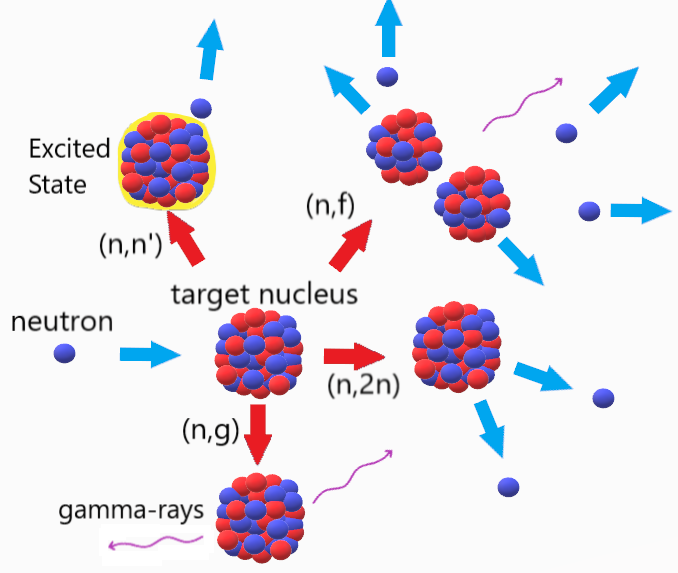
\includegraphics[width=\linewidth]{Figures/Chapter2/NeutronThings.png}
	\caption[Diagram of selected neutron reactions of importance to spectral shaping and fission product generation.]{Diagram of selected neutron reactions of importance to spectral shaping and fission product generation \cite{Greenwood2013}.}
	\label{fig:rxns}
\end{figure}

The neutron interaction probability is described by the neutron microscopic reaction cross-section ($\sigma_{rxn}$), which is a function of the target isotope and incident neutron energy $(E_{n})$.  
The microscopic cross-section multiplied by the atomic number density, $N$, provides the macroscopic cross-section ($\Sigma_{rxn})$, a measure of the interaction probability in bulk material per unit path length traveled. 

% I'd recommend to delete this para.  Sounds good. 
% I don't see where it ties to the following discussion and the fission classification seems a bit early and disconnected.
%Neutrons can be categorized into energy regimes such as thermal, epithermal, and fast, although these regions are relative and vary according to different fields of nuclear sciences or particle physics.  
%A thermal neutron is below 0.025 eV, which is average $E_{n}$, in thermal equilibrium with a 290 K temperature distribution\cite{Duderstadt}. 
%Epithermal neutrons are between 0.025 eV and 1 MeV, and fast neutrons are above 1 MeV.
%In the context of presenting fission product distributions as a function of energy, fast neutrons induce fission under a Watt spectrum at 500 keV, and high energy neutrons are 14 MeV. 

% Need a sentence to preface why the following section is here. As stated, it is unclear what value this para and figure add. I think I'll leave it off to make things condensed. I was going for showing how everything adds up to a total cross-section.  

%The major cross-sections of interest to $^{235}$U up to 20 MeV are displayed in Figure \ref{fig:ntotU}. 
%The total cross-section is the summation of all of the possible reaction mechanisms. 
%Each reaction is explained in further detail below; however, it is important to understand that these reactions are in competition with each other. 
%In general, absorption reactions dominate at low energy. 
%At high energy elastic scattering, inelastic scattering, and (n,xn) reactions are the most probable interaction. 

%\begin{figure}[ht]
%	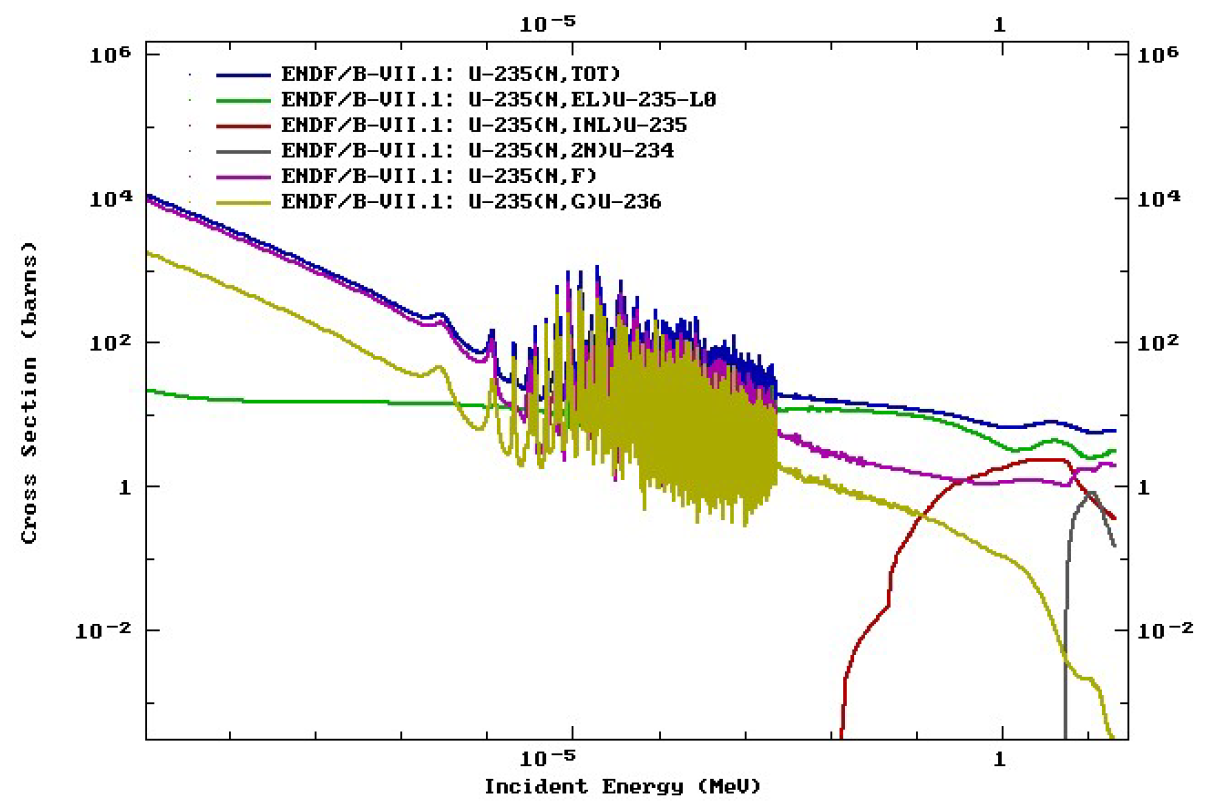
\includegraphics[width=\linewidth]{Figures/Chapter2/n_tot.png}
%	\caption[U-235 (n,f) cross-section compared to competing reaction channels]{U-235 (n,f) cross-section compared to competing reaction channels\cite{ENDF}}
%	\label{fig:ntotU}	
%\end{figure}

\subsection{Elastic Scattering (n,n)}

\ Elastic scattering (n,n) is an extremely important reaction for lowering the average energy of the neutron population by downscattering \cite{Turner}. 
An elastic collision does not place the target nucleus in an excited state, which allows for the simplified use of conservation of energy and momentum to describe the interaction. 
A selected group of elastic scattering cross-sections relevant to the application in the ETA design are shown in Figure \ref{fig:elastic}. 

\begin{figure}[ht]
	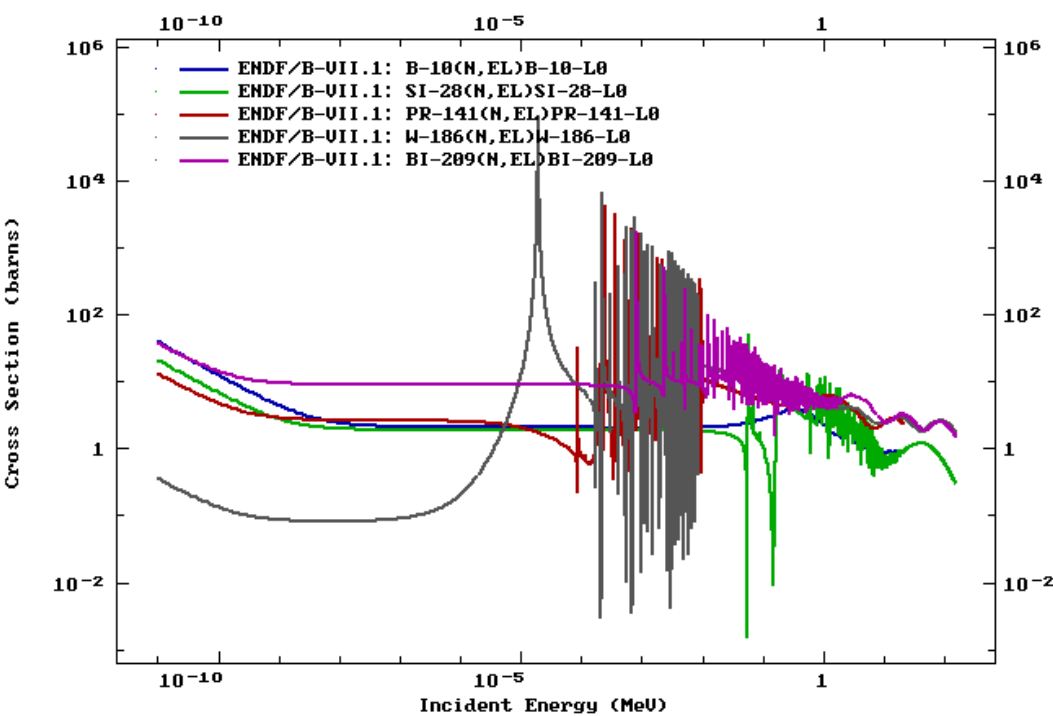
\includegraphics[width=\linewidth]{Figures/Chapter2/elastic.png}
	\caption[Comparison of various elastic scattering cross-sections for materials in the current ETA design]{Comparison of various elastic scattering cross-sections for materials in the current ETA design \cite{ENDF}.}
	\label{fig:elastic}
\end{figure}

\ The maximum energy lost in a neutron elastic collision with a nucleus is a function of the target isotope atomic mass (M). 
Elastic scattering with higher mass isotopes produce a smaller energy loss per collision compared to interactions with low atomic mass nuclei. 
Elastic scattering can transfer nearly all of a neutron's kinetic energy with a collision on hydrogen, while scattering off bismuth will produce very little energy loss. 
The maximum energy transfer (Q) to the target nucleus per collision is given by 

\begin{equation} \label{eq:elastic}
    Q_{max}=\dfrac{4ME_{n}}{(M+1)^{2}}.
\end{equation}
% should define E_n

\subsection{Inelastic Scattering (n,n')}
% This description was a bit off since there are infinite nuclear excited states too (the "continuum". I removed the atomic analogy since it presumed some knowledge about atomic physics; feel free to add back in
\ Inelastic scattering is similar to the reaction dynamics of elastic scattering; however, the target nucleus is placed in an energetically excited state after the impact \cite{Turner}.
The energy of the excited states are governed by quantum mechanics and are unique to particular isotopes. 
An incident neutron, or other particle, can transfer energy to the target nucleus and populate an excited state of the atom.  
For inelastic scattering, this is typically one of the lower discrete energy levels.
However, the incident neutron and target nucleus can form a quasi-continuous spectrum during a compound reaction which gives rise to resonances \cite{Krane}. 
% These resonances have a certain energy width created by states having a energy widths larger than the energy spacing of the states. The width of the resonance is determined by the states. I'm going to delete now. 
% I'm not 100% clear on the last statement 

\ Inelastic scattering is a threshold reaction, meaning an incident neutron must have a minimum amount of energy to enable the reaction channel. 
Additionally, neutrons generally lose more energy per collision with high Z isotopes if the interaction is inelastic compared to elastic scattering. % Is this right? High z tends to have lowere energy states. Changed wording, this is what i meant. 
The energy that would normally be conserved in an elastic collision is reduced in the conservation equations by the energy of the excited state populated. 
Examples of inelastic scattering cross-sections are shown in Figure \ref{fig:inelastic}. %Isotopes from $A=12$ to $209$ are shown to identify the trend of increasing mass number.
% I don't see a trend; I know there is one, but the selected isotopes are all over the place  
% One of them was (g,inl) not (n,inl). fixed 

\begin{figure}[ht]
	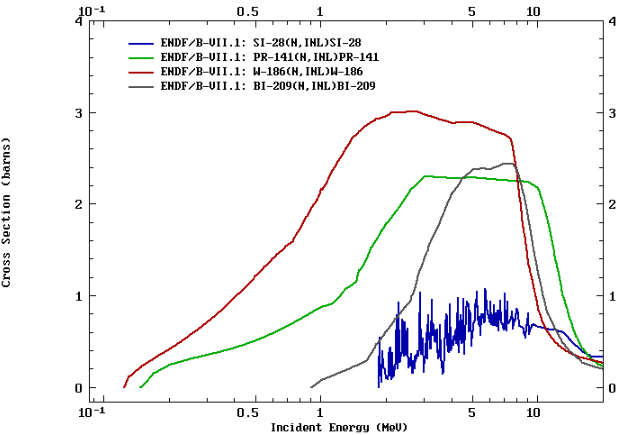
\includegraphics[width=\linewidth]{Figures/Chapter2/inelastic.png}
	\caption[Comparison of various inelastic scattering cross-sections for materials in the current ETA design.]{Comparison of various inelastic scattering cross-sections for materials in the current ETA design \cite{ENDF}.}
	\label{fig:inelastic}
\end{figure}

\ Inelastic scattering is one of the lower threshold energy neutron reactions.
As shown in Figure \ref{fig:inelastic}, there is no general functional form of the threshold energy to enable the reaction by atomic mass. 
The incident neutron threshold energy to cause inelastic scattering with $^{27}$Al, a lighter isotope, is between $^{184}$W and $^{208}$Pb. 
These cross-sections indicate the energy levels of the nuclei itself. 

\ The excited state nucleus can de-excite via gamma emission or other channels if energetically favorable. 
The excited nucleus usually decays in a short time; however, metastable isomeric states can be populated with inelastic scattering and have half-lives on the order of hours or much longer\cite{Krane}. 
These isomeric states have applications in foil activation experiments used for neutron spectrum unfolding, where it may take some time to start measuring the foil activity. 
An energy level and decay mode diagram of $^{115}$In is shown in Figure \ref{fig:In115Rxn}. This isotope is chosen as a representative example because it was used as an activation foil reaction in the modeled ETA results.
The metastable state at 336 keV with spin parity $J^{\pi} = 1/2^{-}$ is important for foil activation experiments for the higher epithermal region.
% Shouldn't this be 115In since that is the (n,n') reaction that you use? Yes, that makes more sense. I think I originally had intended to do something else with this. 

\begin{figure}[ht]
	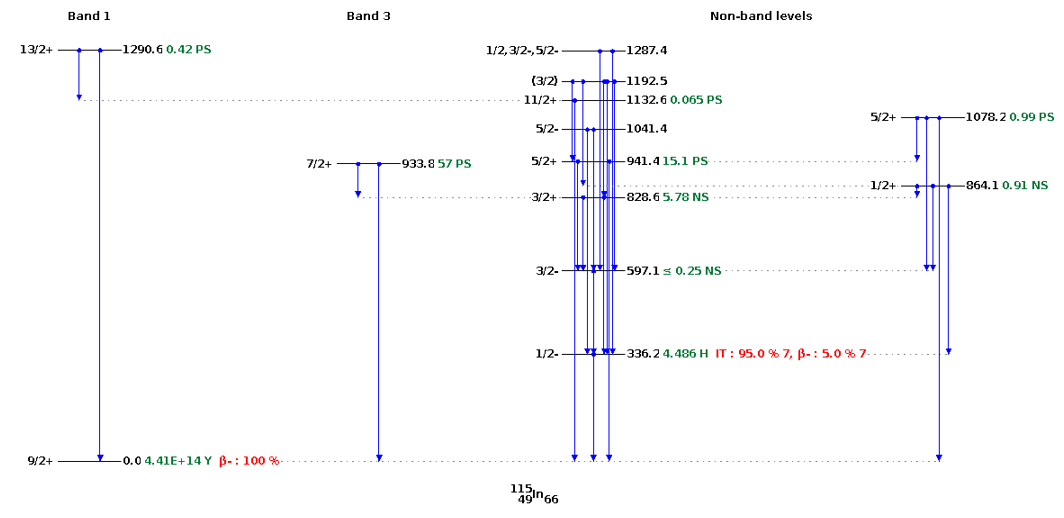
\includegraphics[width=\linewidth]{Figures/Chapter2/TruncatedIn115.png}
	\caption[$\mathrm{^{115}}$In energy level and decay mode diagram truncated at 1.3 MeV.]{$\mathbf{^{115}}$In energy level and decay mode diagram truncated at 1.3 MeV. Plots produced using the Online Service retrieval code package written by C. L. Dunford, National Nuclear Data Center, Brookhaven National Laboratory.}
	\label{fig:In115Rxn}
\end{figure}

\subsection{Neutron Evaporation (n,xn)}

\ A neutron can interact with a nucleus and eject additional neutrons. 
The (n,xn) reactions such as (n,2n) and (n,3n) require a threshold energy to separate the neutron from the original nucleus, appropriately called the neutron separation energy. 
Neutron separation energies are on the order of a few MeV to tens of MeV \cite{Krane,n2ns}. 
Increasing the incident neutron energy allows for the evaporation of more neutrons from the nucleus. 

\ The (n,xn) mechanism can occur as a direct reaction, where the incident neutron interacts with only a few particles in the nucleus, or as a compound reaction, where the incident neutron interact with the entire nucleus and is absorbed \cite{Turner}. 
Example (n,2n) reactions are shown in Figure \ref{fig:n2n}. 
The cross-section threshold is generally lower for higher atomic mass isotopes, which have neutrons that are not as tightly bound to the nucleus. 

\begin{figure}[ht]
	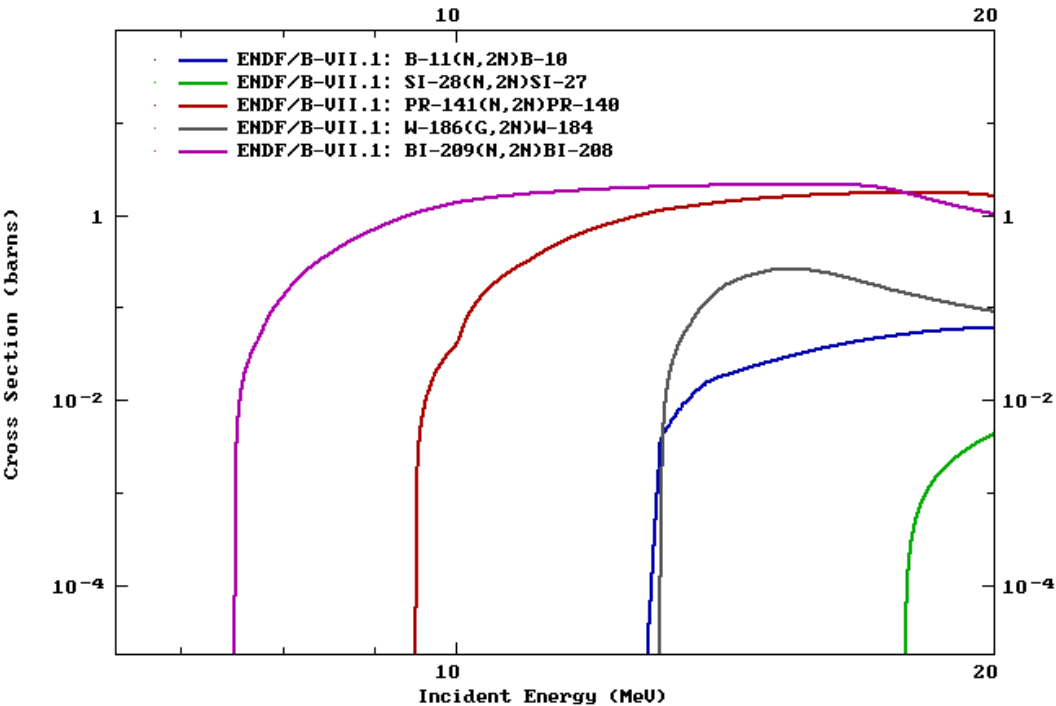
\includegraphics[width=\linewidth]{Figures/Chapter2/n2n.png}
	\caption[Comparison of various (n,2n) cross-sections for materials in the current ETA.]{Comparison of various (n,2n) cross-sections for materials in the current ETA\cite{ENDF}.}
	\label{fig:n2n}
\end{figure}

\ In the context of spectral shaping, (n,xn) reactions are significant for two reasons. 
First, the interaction increases the total neutron population by sacrificing a high energy neutron. 
Second, the neutron energies are lower post-reaction because the reaction is required to overcome the potential barrier and losses through gamma emission. 
% It turns out, for compound rxs, that the emitted neutrons are have a Watt (evaporative) energy distribution 
The lowered neutron energy is beneficial for building up lower energy neutron populations. 
Additionally, this reaction mechanism has applications in foil activation experiments for determining the high energy neutron population.  

\subsection{Radiative Capture (n,$\gamma$)}

Radiative capture, labeled (n,g) and (n,$\gamma$) in literature, is a reaction mechanism most prominent at low energies where an incident neutron is absorbed into the nucleus and a gamma-ray is emitted \cite{Krane}. 
At low energies (below approximately 1 keV, isotope dependent) the absorption cross-section follows the ``1/v" law, so the probability increases with the inverse of the square of $E_{n}$ \cite{Turner}. 
Figure \ref{fig:ngamma} provides examples of selected (n,$\gamma$) cross-sections. 

\begin{figure}[ht]
	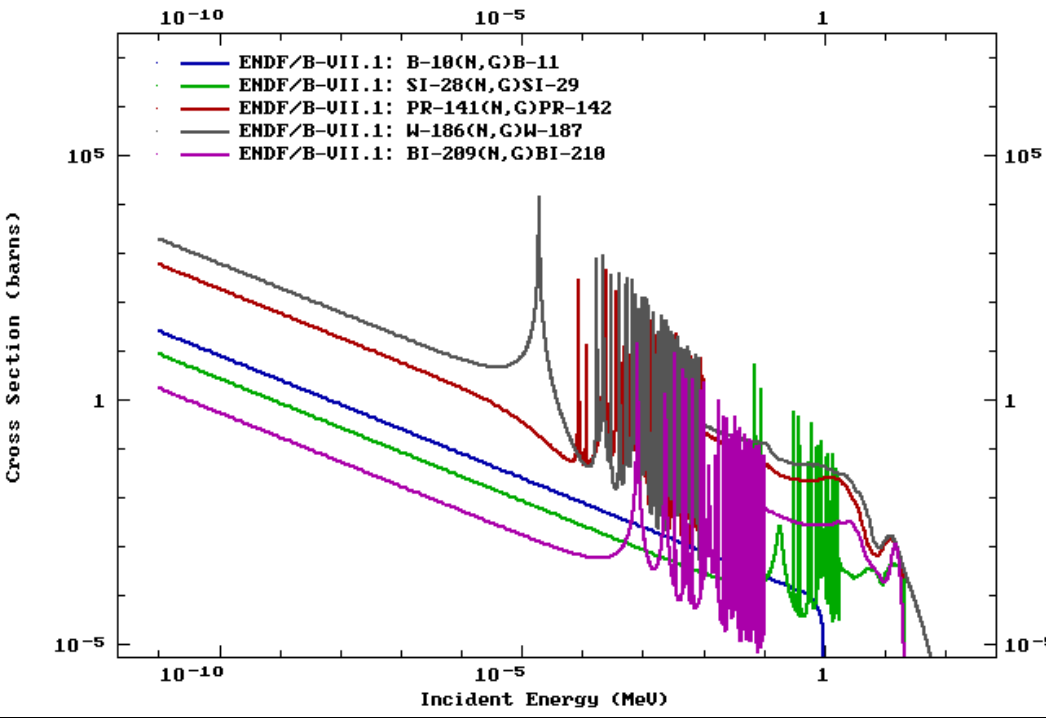
\includegraphics[width=\linewidth]{Figures/Chapter2/ngamma.png}
	\caption[Comparison of various (n,$\gamma$) cross-sections for materials in the current ETA.]{Comparison of various (n,$\gamma$) cross-sections for materials in the current ETA \cite{ENDF}.}
	\label{fig:ngamma}	
\end{figure}

\ Radiative capture is an important absorption reaction mechanism in a few ways. 
The (n,$\gamma$) reactions are of interest to foil activation experiments, specifically for determining the thermal spectrum. 
The resonance structure of the cross-section in the epithermal region can also be used to generate a unique response. 
Radiative capture is generally undesirable for spectral shaping, acting as a poison to the neutron economy. 
Fortunately, the 14 MeV NIF source, is not largely impacted by radiative capture until the neutrons have been moderated, but the ($n,\gamma$) reaction can be used to absorb excess thermal neutrons \cite{Bevins, Krane}. 

\section{Nuclear Fission}
\subsection{Fission Theory}
\ In nuclear fission an excited nucleus breaks up into two or more fission fragments. 
Fission releases a large amount of energy, which is distributed as kinetic energy in the fission fragments, neutrons, gamma-rays, and delayed decay energy. 
The amount of energy liberated is dependent on the specific reaction products and incident neutron energy, so an average number  (approximately 200 MeV) is usually given.
The delayed decay energy is associated with the decay of the unstable fission products, which includes energy in the form of beta ($\beta$) particles, additional gamma-rays, anti-neutrinos, and neutrons. 
A schematic of the fission process is shown in Figure \ref{fig:fission}.

\begin{figure}[ht]
	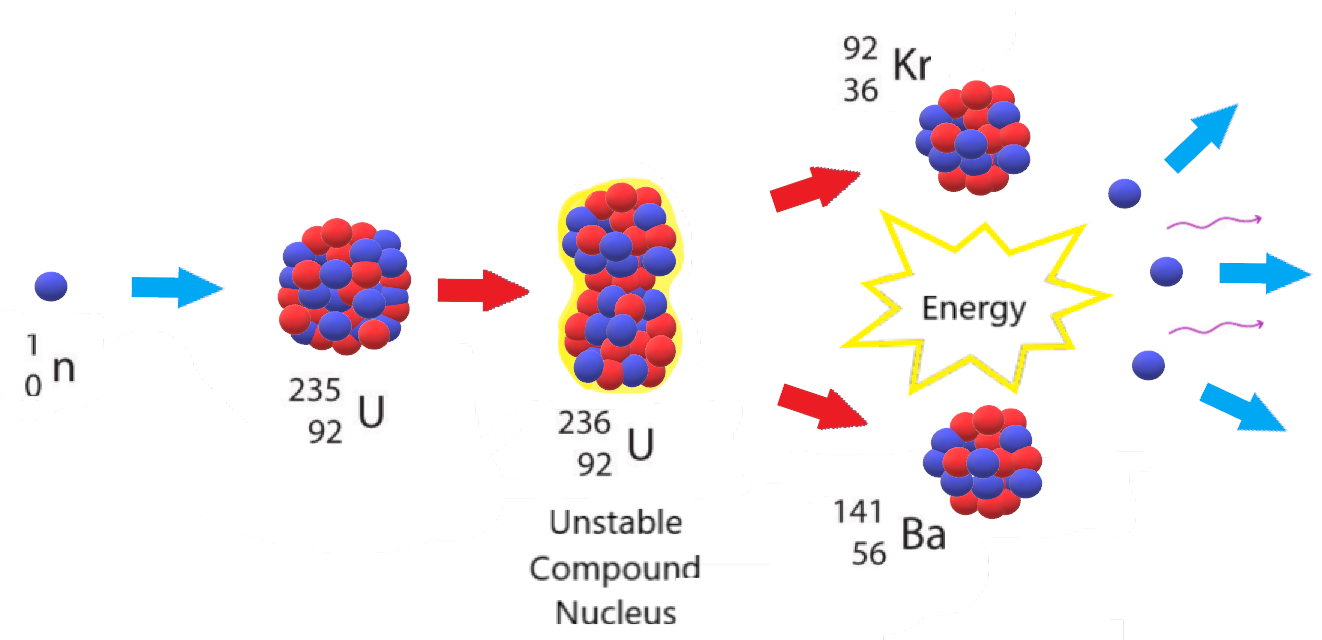
\includegraphics[width=\linewidth]{Figures/Chapter2/Fission.png}
	\caption{Schematic overview of $^{235}$U neutron induced fission. }
	\label{fig:fission}	
\end{figure}

Fission occurs most often in high atomic mass nuclei, such as $^{235}$U, $^{238}$U, or $^{239}$Pu; however, any isotope can be fissioned at large enough incident energies. 
The fissioned isotope separates into two or occasionally three nuclei\cite{Bridgman}. 
Fissionable isotopes like $^{238}$U, $^{240}$Pu, $^{242}$Pu have a significant fission barrier and are incapable of sustaining a nuclear chain reaction. 
Fissile isotopes like $^{235}$U and $^{239}$Pu are capable of sustaining a nuclear chain reaction and have cross-sections with similar characteristics to the radiative capture cross-section shown in Figure \ref{fig:ngamma}. 

The unstable compound nucleus can be modeled at high excitation energies, well above the fission barrier, as an incompressible liquid drop\cite{Krane,Tonchev0}. 
The deformation of the nucleus causes increased surface energies, which are balanced with the Coulomb force (charge repulsion), the strong  nuclear force, and shell pairing effects. 
The perturbation creates an increase in the surface energy and decrease in the Coulomb repulsion because the charge is spread out\cite{Randrup2012}. 
During the fission process, the evolving compound nucleus can emit pre-fission neutrons, known as multi-chance fission \cite{Randrup2012}. 
First-chance fission is the emission of no neutrons, second-chance fission is the emission of one neutron, and so on.  
Multi-chance fission is of particular importance to the mass chains observed in the fission product distribution.

Immediately following the fission event, the fission fragments are in a highly excited state.
Fission fragments are generally very neutron rich compared to the valley of stability. 
The excited fragments emit photons to de-excite and may have enough energy to evaporate more neutrons \cite{Randrup2012}. 
The prompt fission product yield is the distribution of products post neutron evaporation from the fission fragments.  
The fission process releases 2-3 neutrons on average, and this average increases with incident neutron energy due to multi-chance fission and an increase in fission fragment excitation energy. 

\subsection{Fission Products}

The fission product distribution of thermally induced fission tends to be centered around isotopes with closed nuclear shells. 
These isotopes  have a ``magic number" of protons and neutrons, similar to the filled electron structure of the noble gases. 
The fission fragment distribution from thermal neutrons incident on $^{235}$U is shown in Figure \ref{fig:GEF_U}. 

\begin{figure}[htb!]
	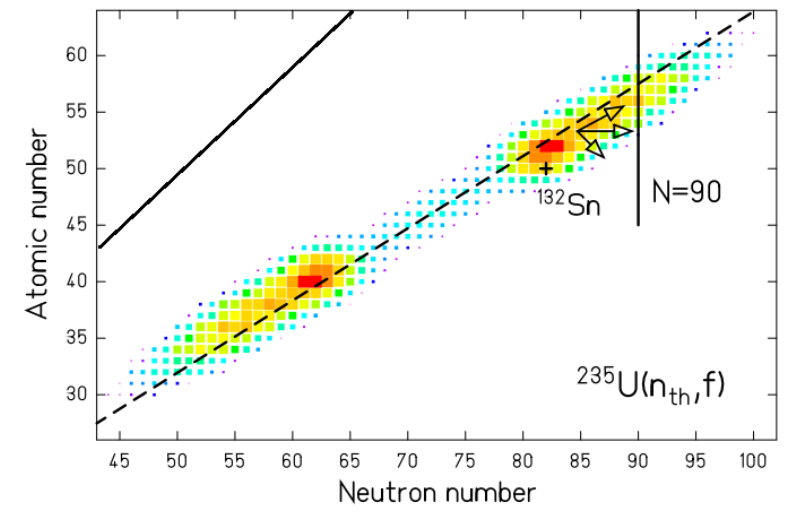
\includegraphics[width=\linewidth]{Figures/Chapter2/U_235Band.png}
	\caption[GEF calculated $\mathrm{^{235}}$U thermal fission product distribution prior to prompt neutron emission.]{GEF calculated $\mathbf{^{235}}$U thermal fission product distribution prior to prompt neutron emission. The dashed line is the neutron to proton ratio of $\mathbf{^{235}}$U prompt fission products and the solid line in the upper left is a ratio of 1\cite{Schmidt2014}.}
	\label{fig:GEF_U}	
\end{figure}

Low-Z stable nuclei have approximately equal numbers of protons and neutrons, but larger nuclei require more neutrons to mitigate the Coulomb repulsion of protons \cite{Krane}. 
Most of the decay products following fission are beta emitters, which occurs because the products are neutron-rich and become more stable upon the conversion of a neutron to a proton. 
Figure \ref{fig:DMode} shows the primary decay modes of isotopes as they decay to the valley of stability. 
In the region of fission products, the primary competing decay mode to $\beta{-}$ is neutron emission, resulting in cross-mass chain transfers after the initial fission process. 

\begin{figure}[htb!]
	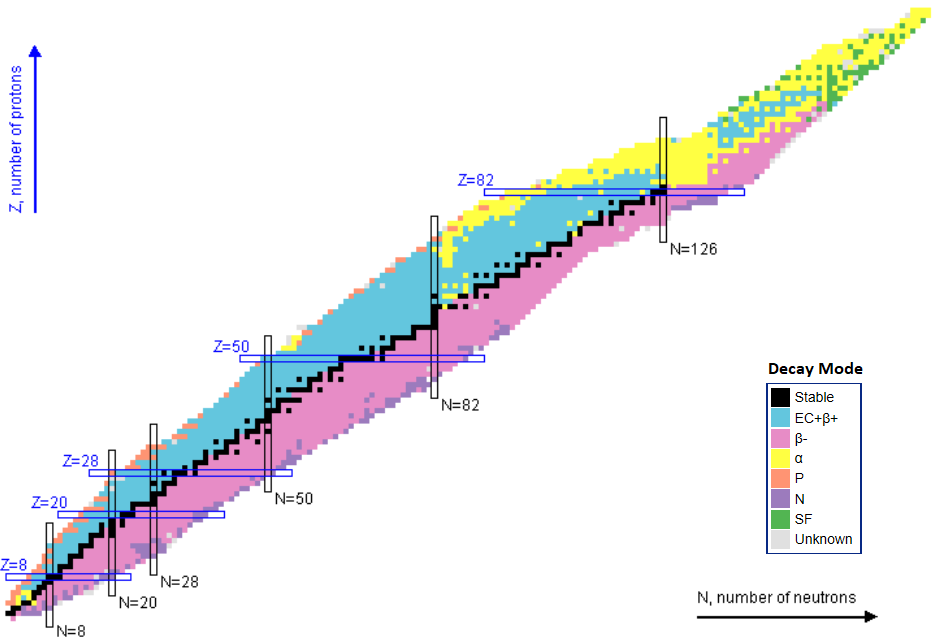
\includegraphics[width=\linewidth]{Figures/Chapter2/DecayModes.png}
	\caption[Primary decay modes of isotopes.]{Primary decay modes of isotopes. Plots produced using the Online Service retrieval code package written by C. L. Dunford, National Nuclear Data Center, Brookhaven National Laboratory.}
	\label{fig:DMode}
\end{figure}

Fission yields can be described by the independent, cumulative, and chain yields. 
The independent yield, $Y_{ind}$, is the prompt fission product distribution directly after the fission event before successive decay \cite{Nichols2008}.
$Y_{ind}$ for $^{235}$U thermal fission is shown in Figure \ref{fig:indy}.
The independent isomeric yield is defined as \cite{indy}

\begin{equation} \label{eq:Indy}
Y_{ind}(A,Z,I) = Y(A) \ \ f(A,Z) \ \ R(A,Z,I), 
\end{equation}

\noindent where the sum yield ($Y(A)$) is the sum of all independent fission products for a given mass A, the isomeric yield ratio ($R(A,Z,I)$) is the the production of each isomer ($I$) for a given independent yield, and the the fractional independent yield ($f(A,Z)$) defines the yield of a particular isotope. 

\begin{figure}[htb!]
	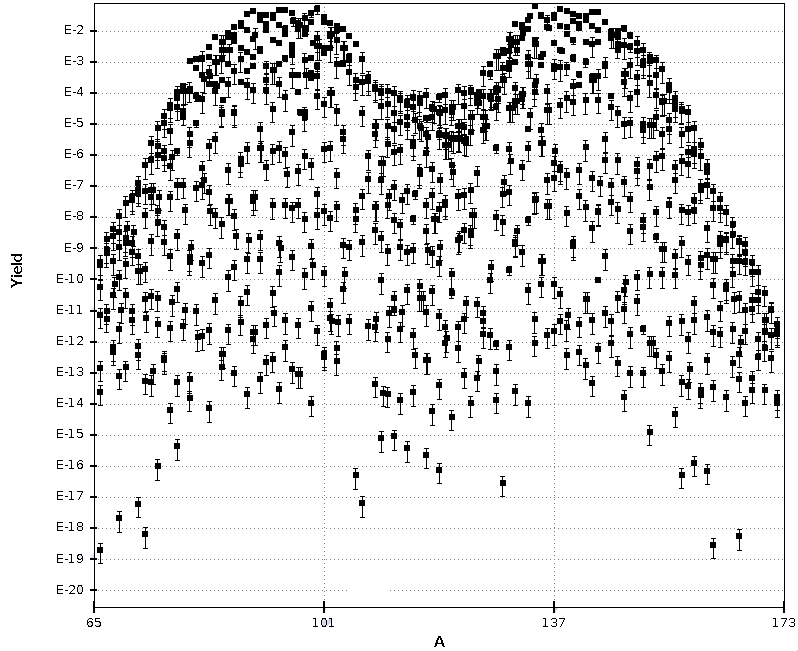
\includegraphics[width=\linewidth]{Figures/Chapter2/indfy.png}
	\caption[Independent fission product yield of thermal fission of $\mathrm{^{235}}$U]{Independent fission product yield of thermal fission of $\mathbf{^{235}}$U. Plots produced using the Online Service retrieval code package written by C. L. Dunford, National Nuclear Data Center, Brookhaven National Laboratory.}
	\label{fig:indy}
\end{figure}

The independent yield produces a cascade of decay chains leading to the cumulative yield, $Y_{c}(A,Z,I)$. $Y_{c}$ represents the production of an isotope over all time after all prompt and delayed emissions and decays. $Y_{c}$ is normally the quantity that is measured in experiments. The cumulative yield is given as \cite{Privas2016}

\begin{equation} \label{eq:Cumulative}
Y_{c}(A,Z,I) = Y_{ind}(A,Z,I) + \sum_{j=0}^N Y_{c}(A_{j},Z_{j},I_{j}) \; b_{j}.
\end{equation}

\noindent where $b_{j}$ represents the branching ratio from isotope $j$ into the cumulative yield and $N$ defines the total number of decay channels into the cumulative yield isotope. 
The cumulative yields for thermal, fast, and high energy fission of $^{235}$U are shown in Figure \ref{fig:U235Cumulative}. 

\begin{figure}[htb!]
	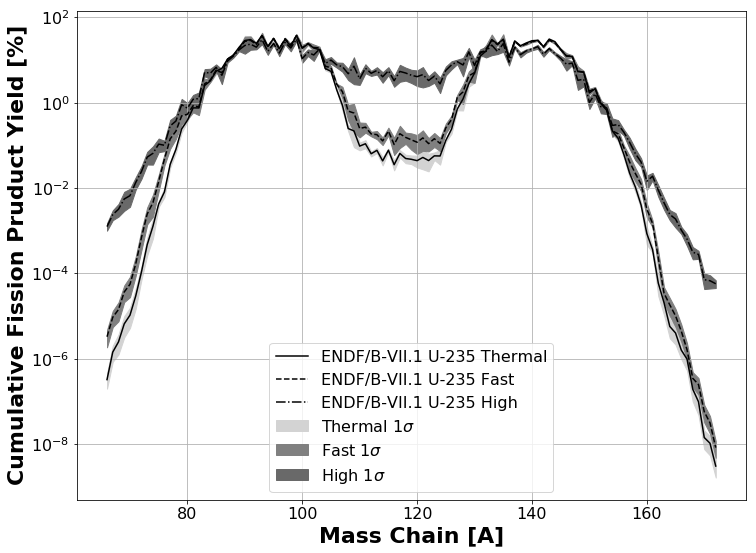
\includegraphics[width=\linewidth]{Figures/Chapter2/ENDF_FPs.png}
	\caption[Comparison of energy dependent${^{235}}$U cumulative fission product distributions]{Comparison of energy dependent $\mathbf{^{235}}$U cumulative fission product distributions from ENDF/B-VII.1 \cite{ENDF}.}
	\label{fig:U235Cumulative}	
\end{figure}

% This makes way more sense with Walid's lecture notes. I am leaving out sum chains, because they are not used. - glad they helped!
As shown in Figure \ref{fig:U235Cumulative}, fission product yields are dependent on the energy of the incident neutron and the identity of the fissioning nucleus. 
The fission products populate one heavy and one light peak. 
The region between the peaks is referred to in this work as the valley, and the low population tails falling off either peak are the wings. 
As the energy of the incident neutron is increased, the valley and wings of the fission product distribution are raised because the fission process becomes more symmetric \cite{Tonchev0}. 
The uncertainty in the fission product yields varies significantly; the fast fission relative uncertainty ranges from 1.6\% for mass chain 137 to 64\% for mass chain 109 \cite{ENDF}. The uncertainty for each fission product is representated at the 1$\sigma$ level as bands in Figure \ref{fig:U235Cumulative}.

\ Finally, the chain yield for a particular mass chain is defined as the sum of the cumulative yields to the final decay to a stable isotope in that mass chain \cite{Nichols2008}. 
The chain yield leads to the cumulative distribution accounting for branching in and out of a mass chain through neutron emission.
In particular, the chain yield equals the cumulative yield for the last stable member of a decay chain.  
An example is shown in Figure \ref{fig:89} for the A = 89 mass chain, where the stable isotope is Y-89\cite{SINGH20131}. 
The neutron deficient decay scheme has not been shown as it has negligible contribution to the fission product decay scheme. 

\begin{figure}[htb!]
	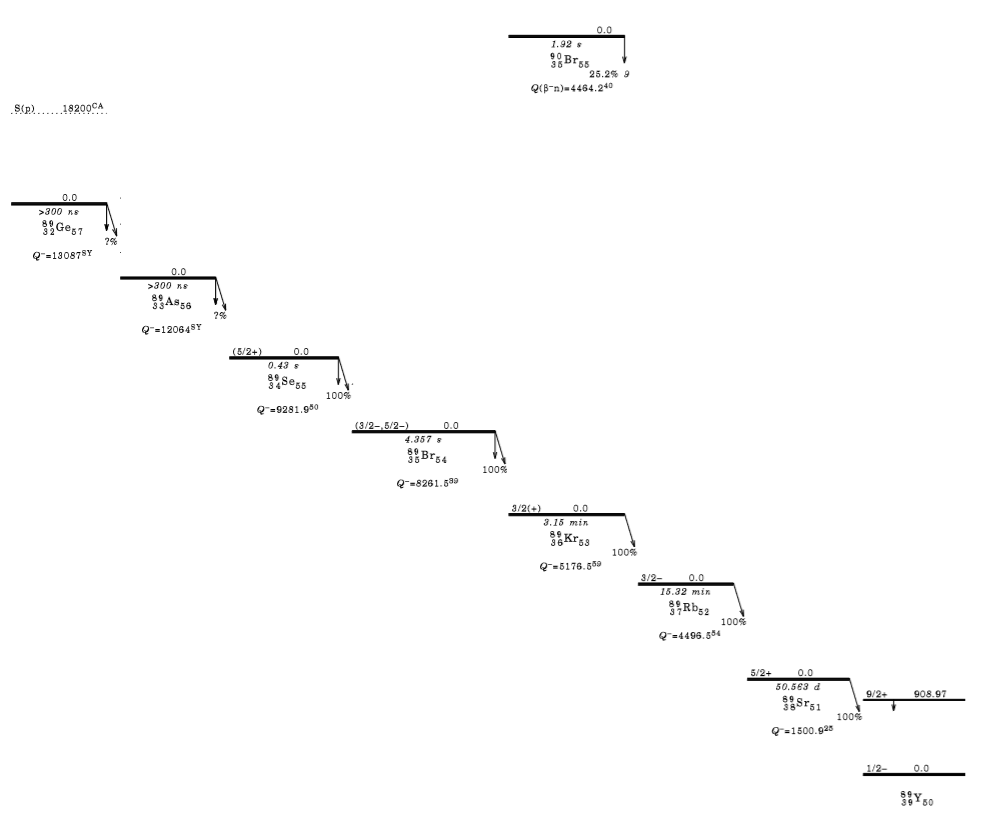
\includegraphics[width=\linewidth]{Figures/Chapter2/89MassChain.png}
	\caption[Simplified neutron rich decay scheme for mass chain A=89. The $\mathrm{^{89}}$Sr decay to $\mathrm{^{89}}$Y represents the final decay to the stable isotope.]{Simplified neutron rich decay scheme for mass chain A=89. The $\mathbf{^{89}}$Sr decay to $\mathbf{^{89}}$Y represents the final decay to the stable isotope \cite{SINGH20131}.}
		\label{fig:89}	
\end{figure}

%The radioactive emissions of the final decay can be used to measure the cumulative fission product yield for an isotope. 
%Some mass chains are more well-behaved for measuring the cumulative yield. For example, the $A=89$ mass chain has many decays that have very short half-lives, up to the precursor stage for the stable isotope. 

% This feels like this should be in Ch1 and is a bit out of place here. Rolling from the disscusion of FPs into how to predict the yield flows better IMO. Moved to Intro

\subsection{Nagy Fits for Fission Product Isotopes}

% I would add a transition sentence to tie the three formalized fissioning energies shown in Fig 12 to this section and motivate why fitting empirical data is needed or makes sense.
The three fissioning isotope energies provided in ENDF describe part of the behavior of the fissioning system as a function of neutron energy.
However, including fits to experimental data enables better energy resolution and predictions consistent that are consistent with observed experiments.  
Empirical relations developed by Nagy, \textit{et al.} provide an approach to predict the fission product yield as a function of energy given sufficient yield measurement data \cite{Nagy1978}.
Nagy fits the fission product experimental data to an exponential equation 

\begin{equation} \label{eq:nagy}
Y(E_{n}) = Y_{0}e^{bE_{n}}.
\end{equation}
where the fitting parameters $b$ and $Y_{0}$ represent the slope of the function in logarithmic form and thermal fission yield, respectively\cite{Nagy1978}. 
The slope is the primary measure of the energy dependency of the fission product yield, which requires  modifications for multi-chance fission.
First chance fission is dominant from up to 5.5 MeV, and second-chance fission up to 14.1 MeV\cite{Nagy1978}. 
Multi-chance fission effects on the fission product yield are less pronounced in asymmetric regions but can have a large impact in symmetric fission ($109 \leq A \leq 129$)\cite{Bevins}\cite{Nagy1978}. 

It is important to note that data-based phenomenological models are not perfect predictors of determining fission products \textit{a priori}. 
In particular, recent publications have findings that cannot be accurately modeled with current theoretical approaches \cite{Tonchev0}. 
In general, there are large uncertainties in the predictive power of calculating energy dependent fission product yields. 
Still, this type of empirical fit has lower predicted error than GEF for individual isotopes where sufficient energy-dependent measurements exist. 

\section{Nuclear Data}
\subsection{Nuclear Data Libraries}

\ Nuclear data relevant to neutrons has been collected for the better part of the last century. 
Nuclear data available for modeling and simulations is collected and published in evaluated data files. 
% Technically the experimental data is published in EXFOR, which the evaluators use to generate the evaluated data files.
There are many versions of evaluated nuclear data, which all aim to characterize the relevant physics backed by experimental results. 
For example, the primary U.S.-based nuclear data file is the Evaluated Nuclear Data File (ENDF). 
Other nations or organizations also have independent evaluations of the available nuclear data. 
Examples of other nuclear data libraries are the Russian National Library of Nuclear Data (ROSFOND), the European Joint Evaluated Fission and Fusion (JEFF) Nuclear Data Library, Japanese Evaluated Nuclear Data Library (JENDL), Chinese Evaluated Nuclear Data Library (CENDL), and the International Reactor Dosimetry and Fusion File (IRDFF).

Figure \ref{fig:RxnComp} shows the evaluation of $^{197}$Au (n,2n) reaction for various libraries. 
In some cases, the library evaluation can be drastically different. 
However, sometimes the libraries are drawing from the same data and models, which can be noted by the overlapping evaluations. 

\begin{figure}[ht]
	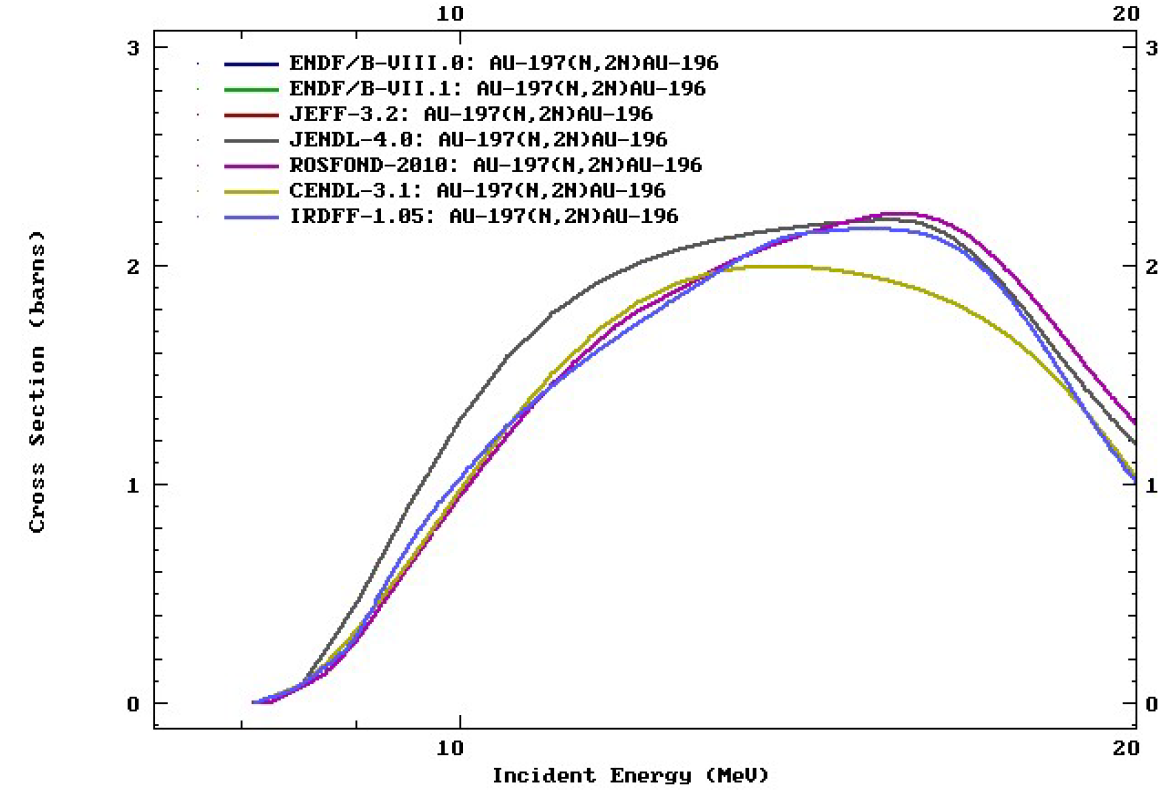
\includegraphics[width=\linewidth]{Figures/Chapter2/RxnComp.png}
	\caption[Comparison of various library evaluations of the  $^{197}$Au (n,2n) cross-section.]{Comparison of various library evaluations of the $\mathbf{^{197}}$Au (n,2n) cross-section \cite{ENDF}.}
	\label{fig:RxnComp}
\end{figure}

\ The experimental data that feeds into ENDF is contained in EXchange FORmat (EXFOR), where the experiment uncertainty, if available, is tracked.
Nuclear data evaluators need reaction models to fill in the gaps where experimental data does not exist.  For example, experiments with sub-electron-volt neutron energy resolution are not feasible at the present time. 
ENDF relies on evaluations of EXFOR data based on experimental quality, statistics, and theoretical basis to fill in areas lacking experimental data \cite{Brown2015}. 
ENDF then stores the underlying nuclear data (cross-sections, angular distributions, half-lives, ect.) that can be used in simulations. 

\ Benchmarking the evaluated nuclear data is done primarily through testing integral results, such as the effective neutron gain-to-loss ratio ($k_{eff}$) of a critical assembly \cite{Brown2015}. These integral measurements provide a more accessible measurement that can be done with high precision and accuracy, as precise as a relative error of 0.01\%, to validate microscopic cross-sections. The use of integral benchmark experiments is important for comparing the net result of the nuclear data; however, there are uncertainties and correlations in the independent reactions that combine to create the integral results. 

\ Validation experiments, applications, studies, and integral benchmarks performed increase the base and accuracy of the nuclear data\cite{Brown2015}.
However, it is important to note that the experiments used to measure nuclear data may have uncertainties that vary by orders of magnitude. An interesting feature of this fact is that the relative nuclear data uncertainty does not always decrease between successive library versions. One example is the increase in uncertainty in the neutrons released per thermal fission of $^{235}$U, which increased from 0.311\% to 0.385\% between ENDF/B-VII.0 to VII.1 \cite{Bostelmann2017}. Another example demonstrating the nuclear data uncertainty is that evaluated $\mathrm{^{6}}$He half-life has changed by approximately 5\% with large increases in the relative error over the last 50 years\cite{he6}.

\  Another prevalent issue is that the majority of accurate measurements were performed for nuclear reactor studies, which limits accessibility to reliable data in different energy domains. As a consequence of this, ENDF only contains fission production data at thermal, fast (0.5 MeV), and high energy (14 MeV). To combat this challenge, smaller, more application-specific libraries have been developed. 

\ The International Atomic Energy Agency (IAEA) provides data to the benchmarked neutron dosimetry reaction IRDFF library \cite{IRDFF}. This library is noted because it is used in the PNNL STAYSL code system, discussed in Section \ref{STAYSLthing}. The IRDFF v.1.05 library contains ``state-of-the-art" covariance information and has improvement through testing and integral experiments \cite{Greenwood2017}. 

\ The IRDFF library also includes feed through from fast decaying excited states to metastable states for important dosimetry reactions. An example is the $\mathrm{^{115}}$In (n,n') $\mathrm{^{115m1}}$In reaction; the $\mathrm{^{115m1}}$In decay scheme os depicted in Figure \ref{fig:In115Rxn}. 
% If you change figure 5 as suggested, you need to change this example accordingly.
The first metastable state at 336 keV (spin parity $J^{\pi}$ = $1/2^{-}$) has a half-life of 4.5 hours, which makes it a good candidate reaction for foil activation experiments \cite{Zolotarev2013}. 
The IRDFF v.1.05 library contains reaction data that includes the decay of additional metastable states and higher excited states into $\mathrm{^{115m1}}$In. 
%$\mathrm{^{116m2}}$In decays to $\mathrm{^{116m1}}$In with a 2 second half-life. 
Under standard measurement timing conditions, all of the higher energy $\mathrm{^{115}}$In states will have decayed, thus contributing to the activity measured for the first metastable state. 
% This is why I picked 116. 115m does not have multiple excited states. 

\subsection{Nuclear Data Covariance}

\ Covariance arises in nuclear related experiments when one process affects another or the nuclear data measurement energy ranges are correlated. 
Unfortunately, nuclear data covariance analysis is not standard to experimental analysis. Often errors are attributed to model fidelity, measurement, or setup problems when nuclear data covariance may have been the root cause \cite{edsdoj111}. 
In many nuclear decay processes, the correlation between decays is unity because the decays happen in a series. 
However, covariance can occur if there is branching from a radioactive state. 
Covariance is defined with the expectation values, $\left\langle X \right\rangle$, and mean value ($\mu$) providing for the covariance between variables X and Y as
 
\begin{equation} \label{eq:Cov1}
      cov(X,Y) = \left\langle  XY \right\rangle-\mu_{X}\mu_{Y}, 
\end{equation}

\ A correlation matrix combined with the uncertainty in the nuclear data can be used to form the covariance matrix. 
The diagonal of the correlation matrix is 1, so the diagonal of the covariance matrix is the variance for the group.  As such, the covariance of an observable compared to itself reduces to the variance 

\begin{equation} \label{eq:Cov2}
      cov(X,X) = \left\langle  X^{2} \right\rangle-\left\langle  X \right\rangle^{2} = \sigma_{X}^{2}.
\end{equation}

\noindent The conversion from a correlation matrix to a covariance matrix is given by

\begin{equation} \label{eq:Cov3}
cov(X,Y) = corr(X,Y) \sigma_{X} \sigma_{Y}. 
\end{equation}

\ Instead of the covariance matrix, nuclear data often stores the correlation matrix in a group structure format, as shown in Figure \ref{fig:coor}. In general the largest correlations occur in nearby energy groups, where the experimental uncertainty in the incident $E_{n}$ is largest. Correlations also exist between reactions, in addition to correlations in a single energy-dependent reaction channel, but this data is rarely quantified.
% At least that I know of it isn't quantified. SCALE has some info on it, but there is not a lot. 

\begin{figure}[htb!]
	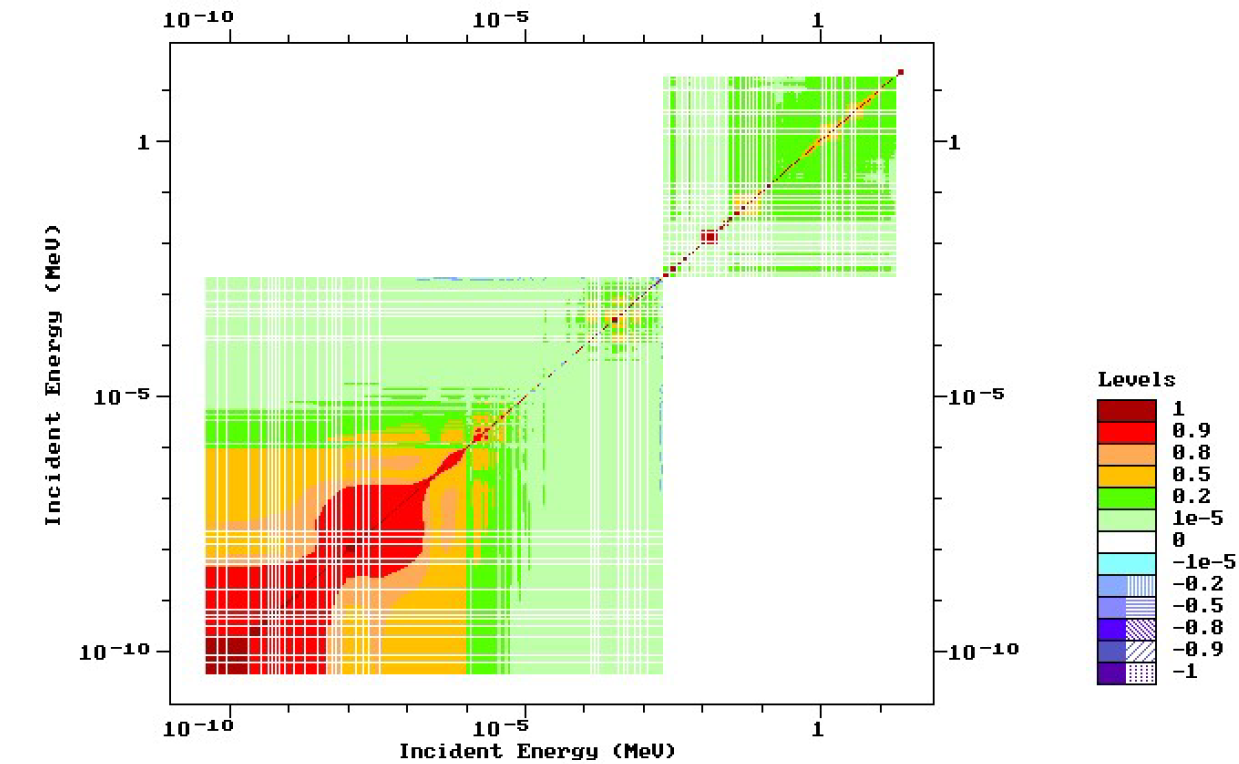
\includegraphics[width=\linewidth]{Figures/Chapter2/U235_nf_coor.png}
	\caption[$\mathrm{^{235}}$U (n,f) correlation matrix.]{$\mathrm{^{235}}$U (n,f) correlation matrix\cite{ENDF}.}
	\label{fig:coor}
\end{figure}

\ Integral experiments are extremely dependent on the underlying reactions that make up the net result. 
Therefore, there are generally larger variances in the the reactions that are part of the total cross-section. 
Figure \ref{fig:U235rel} displays the relative uncertainty of the $\mathrm{^{235}}$U (n,f) cross-section compared to the total cross-section. 
Figure \ref{fig:Bi209rel} displays the relative uncertainty of the total cross-section of $\mathrm{^{209}}$Bi compared to the (n,2n) reaction cross-section. 

\begin{figure}[htb!]
	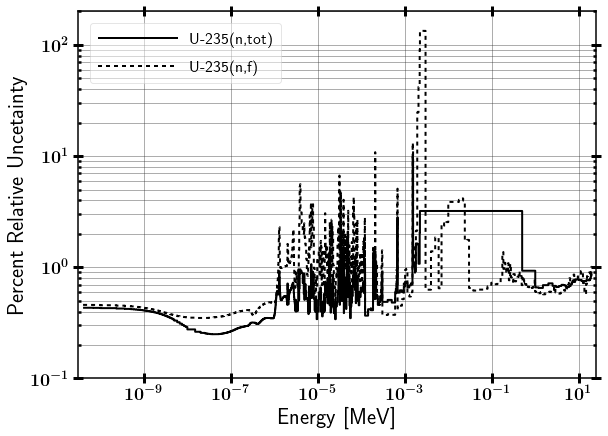
\includegraphics[width=0.9\linewidth]{Figures/Chapter2/U235_RelUncert.png}
	\caption[Percent relative uncertainty in $\mathrm{^{235}}$U (n,f) cross-section compared to $\mathrm{^{235}}$U (n,tot) cross-section]{Percent relative uncertainty in $\mathbf{^{235}}$U (n,f) cross-section compared to $\mathbf{^{235}}U$ (n,tot) cross-sections \cite{ENDF}.}
	\label{fig:U235rel}
\end{figure}

\begin{figure}[htb!]
	\includegraphics[width=0.9\linewidth]{Figures/Chapter2/Bi_209_RelUncert.png}
	\caption[Percent relative uncertainty in $\mathrm{^{209}}$Bi (n,2n) cross-section compared to $\mathrm{^{209}}$Bi (n,tot) cross-sections]{Percent relative uncertainty in $\mathbf{^{209}}$Bi (n,2n) cross-section compared to $\mathbf{^{209}}$Bi (n,tot) cross-sections \cite{ENDF}.}
	\label{fig:Bi209rel}
\end{figure}

\ The uncertainty in $\mathrm{^{235}}$U (n,f)  and $\mathrm{^{209}}$Bi highlight a couple key attributes relevant to nuclear data. 
First, the component reactions that make up the total cross-section almost always have a higher relative uncertainty because integral cross-section experiments can more accurately be measured through attenuation of a ``beam" of neutrons. 
The underlying reactions are generally more difficult to characterize. 
Second, the $\mathrm{^{235}}$U (n,f) cross-section relative uncertainty near 2.2 keV is 133.6\%. 
This large uncertainty implies that the cross-section must go negative to capture the full distribution of possible total cross-sections within a given confidence interval when utilizing a Gaussian distribution.
This suggests that the confidence intervals are not symmetric and points to utilizing alternative functional forms for the cross-section probability distribution functions. 
% Have you seen anything that would indicate the uncertainties assigned are not assuming a gaussian distribution? 
% Yes somewhat. I know all of the codes sample from a multivariate normal distribution, but:
% From ENDF - It is not necessary to assume that the density functions are normal in shape,
% or otherwise, unless one must estimate the probability that the true value lies within a certain
% range of the expected value.
This is obviously non-physical; however, it gives scope to the magnitude of the uncertainty in the underlying cross-sections over difficult experimental energy ranges. 
Next, the $\mathrm{^{235}}$U reactions are more thoroughly studied as compared to $\mathrm{^{209}}$Bi. 
Over the majority of the energy range, The uncertainty in the $\mathrm{^{235}}$U cross-section is below one percent relative error, largely driven down by thermal nuclear reactor experiments, while $\mathrm{^{209}}$Bi cross-section has a larger error around 5\%. 
Finally, areas where the cross-sections are low have representative larger relative errors; this is the case near the threshold of the $\mathrm{^{209}}$Bi (n,2n) reaction as shown in Figure \ref{fig:Bi209rel}. 

\subsection{Nuclear Data Stochastic Sampling}

\ The two primary methods that exist for uncertainty quantification of radiation transport simulations are linear perturbation and stochastic sampling Monte Carlo approaches \cite{Rochman2011}. 
First order linear perturbation theory is not always adequate for large uncertainties or incorporating second order effects from the uncertainty in the neutron transport; however, it does have broad uses in the reactor community.
Stochastic sampling has grown in popularity as computational resources have improved. 
Stochastic methods rely on performing independent neutron transport calculations with perturbed nuclear data libraries sampled based on the covariance of the cross-sections using the multivariate normal distribution to build a distribution of responses \cite{Aures2017}. 
The generalized multivariate normal distribution is a function of the nuclear cross-section mean values ($\boldsymbol{\mu}$), length \textit{k}, random solution vector ($\boldsymbol{X}$), covariance matrix ($\boldsymbol{\Lambda}$) is given by

\begin{equation} \label{eq:Cov4}
f(\boldsymbol{X}) = \dfrac{exp(-0.5(\mathbf{X}-\boldsymbol{\mu})^{T}\mathbf{\Lambda}^{-1}(\mathbf{X}-\boldsymbol{\mu}))}{\sqrt{(2\pi)^{k}\mid \mathbf{\Lambda} \mid}}.
\end{equation}

\noindent Several Monte Carlo sampling methods have been created to capture the effect of nuclear data covariance on nuclear engineering problems, including SCALE Sampler, NUSS, and SHARK-X \cite{Diez2015, Zhu2015a, SCALE, Aures2017}.  

\ Deficiencies with the stochastic sampling approach are generally associated with the nuclear data libraries and the sampling method. 
First, nuclear data uncertainty is often above 100\% in energy regions where a measurements do not exist, so the value of the cross-section is not well characterized. 
Second, the nuclear data uncertainty is assumed to be normally distributed; however, alternative forms may be more appropriate. 
In stochastic sampling approaches, these two factors lead to truncation of large uncertainties to prevent performing neutron transport calculations with negative cross-sections. 
Although negative cross-sections are non-physical, the truncation may underestimate the calculated uncertainty which can have an effect if the experiment is performed in these energy domains when using the Gaussian distribution. 
Finally, component cross-sections which make up the total cross-section are constrained to sum to the total cross-section. 


\section{Monte Carlo Neutron Transport}
\subsection{Monte Carlo Neutron Transport Theory}
\ Monte Carlo methods for neutron transport leverage pseudo-random sampling, nuclear data, and material specifications to build a simulation of the particle transport in space, direction, energy, and time \cite{Luciano2012a}. 
Neutron interactions are sampled with probability distribution functions (PDFs) for aspects such as path length traveled and interaction type \cite{Lewis1984}. 

\ An objective of a neutron transport calculation is to determine the average behavior of particles with-in the system. 
This can be captured with the volume averaged scalar flux, $\bar{\phi_V}$, defined as

\begin{equation} \label{eq:flux}
\bar{\phi_V} = \frac{1}{V}\int_V dV \int_t dt \int_E dE\: \phi(\vec{r}, E,t),
\end{equation}

\noindent where  $\bar{\phi_V}$ is given as a function of energy ($E$), position ($\vec{r}$) and time ($t$).
Monte Carlo methods approximate the scalar flux with either track length or collision estimates \cite{Lewis1984}. The track length estimator is 

\begin{equation} \label{eq:track}
\bar{\phi_V}  = \frac{W \: T_l}{V \: N},
\end{equation}

\noindent where the path length score for the flux is based on the distance traveled ($T_{l}$) and is normalized by the particle weight (W), cell volume (V), and number of histories sampled (N).

\ Statistics often drive the uncertainty in a Monte Carlo simulation as systematic uncertainties are generally not considered due to computational costs. 
The ``true" mean value, $\mu$, of a response PDF is the expectation value, $E(x)$, which is estimated with a sample mean, $\bar{x}$. 
According to the Central Limit Theorem, the sample mean approaches the real mean as the number of samples, $N$, goes to infinity, and the distribution of sampled $x_i$ follows a Normal distribution.
The sample mean can be calculated as

\begin{equation} \label{eq:sampmean}
\bar{x} = \frac{1}{N}\sum_{i=1}^N x_i. 
\end{equation}

\noindent Therefore, sample variance, ($S_x^2$) can be computed as

\begin{equation} \label{eq:sampvar1}
S_x^2 = \frac{1}{N-1}\sum_{i=1}^N (x_i - \bar{x})^2,
\end{equation}

\noindent and the variance of the mean, ($S_{\bar{x}}^2$), is simply

\begin{equation} \label{eq:sampvar}
S_{\bar{x}}^2 = \frac{S_x^2}{N}, 
\end{equation}

\noindent where $S_x^2$ is defined with the sample variance.  
Therefore, the statistical uncertainty in the results decreases with $\sqrt{N}$. 
The precision of the result can be improved with more histories, shrinking the spread in $x_i$. 
However, the accuracy cannot be improved. 
Accuracy is impacted by systematic errors, such as uncertainty in the nuclear data.

\subsection{Comparison of Monte Carlo Neutron Transport Results}\label{'secMC'}

The results from different Monte Carlo simulation codes often produce slightly different results. The outputs are generally in better agreement for criticality calculations of critical assemblies and nuclear reactor analysis. 
It is important to gauge the effect of utilizing different transport codes to see how much variance is expected. 
Some of the differences that effect Monte Carlo simulations are within the structure of the code itself, statistical error, or different starting seeds, while others are based on the nuclear data that may be altered, geometry or source implementation, or user error.

Criticality is a well-understood nuclear engineering problem that the nuclear data libraries are validated against. 
Wang, \textit{et al.} conducted on a high temperature pebble-bed reactor compared SCALE's CSAS6 module for criticality calculations to MCNP5's kcode\cite{Wang2014}. 
The results showed a difference for calculating $k_{eff}$ to be on the order 0.5\%. 
% Should this be 10^4? Everything I have says 10^5, and wiki
This variance can easily be handled for reactor operations; however, this highlights that even well understood problems do have differences based on simulation code. 
A similar study conducted by Johnson \textit{et al.} of a pebble-bed reactor determined that the difference in $k_{eff}$ in MCNP to SCALE was near half a percent  \cite{Johnson2007}. %With a varied geometry? Yes, they looked at a bunch of configurations to optimize it. I'm taking that out now, it was confusing wording  on my end. --- For what output? keff? 
In another study, Chen \textit{et al.} compared the average gamma-ray dose outside of a spent nuclear fuel cask \cite{Chen2011}. 
The dose rates predicted by SCALE and MCNP simulations varied as much as 27\%. 
Again, this shows that the less benchmarked studies can have large code-to-code disagreements. 

\section{Foil Activation}
\subsection{Foil Activation Theory}

Foil activation is a method of characterizing an incident neutron flux through unfolding the response of the foils using the energy-dependent nuclear reaction channels in the foil. 
Activation experiments are essential for testing that requires small geometries or where electronic equipment used in measuring techniques will be damaged. 

Activation foils produce measurable radioactive isotopes during the course of irradiation. 
The production rate of radioactive isotopes is negated by radioactive decay processes, which place an upper limit on the radioactivity of a foil \cite{Knoll}. 
The saturated activity 

\begin{equation} \label{eq:InfReactionRate}
A_{\infty} = R = \int_{E1}^{E2} \phi(E) \Sigma(E) _{act} V
\end{equation}

\noindent is equivalent to the reaction rate ($R$), which is a function of the energy dependent flux ($\phi$), the macroscopic reaction activation cross-section ($\Sigma(E)_{rxn}$), and the volume of  the foil ($V$). The energy term ($E1$) is zero in many cases; however, threshold reactions require the incident neutron to be of higher energy to enable the reaction channel. 

When six half-lives have elapsed, a foil will have reached approximately 98\% of its saturation activity, neglecting spatial and energy self-shielding effects \cite{Knoll}. 
When the activation is not sufficient to fully saturate the foil, a correction needs to be made.
The activation of the foil for a given irradiation time ($t_{i})$ is given as 

\begin{equation} \label{eq:ReactionRate}
A_{0} = A_{\infty}(1-e^{-\lambda t_{i}}), 
\end{equation}

\noindent where $\lambda$ is of the decay constant of the radioactive product.

The formula can be simplified in the limit of irradiation times much less than 
the half-life of the activation products. In this case, the production rate is 
much larger than the decay from radiation, so the rate of production of the 
radioisotope is driven only by the reaction rate. The neutron pulse length at the NIF is on the order of shakes (1 shake = 10 nanoseconds), while the reaction channels of interest have half-lives on the order of an hour or longer. Therefore this approximation can be made for the foil activation. The time integrated flux, or neutron fluence ($\Phi$), can be used to determine the total reactions, ($R_{total}$),
over an irradiation period, given by

\begin{equation} \label{eq:NIFrxnRate}
R_{total} = \int_{E1}^{E2} \Phi(E) \Sigma(E) _{act} V \:dE.
\end{equation}

% I've tried to make the use of () or ,, for the definition of symbols consistent, but you may want to double check.
Experimental measurements of the activity must be corrected to deduce the original activity of the foil ($A_{0}$) immediately after irradiation as shown in Equation \ref{eq:MeasActivity}. 
The activity is corrected for the radioactive decay occurring between the end of irradiation and the start of counting ($t_{d}$). 
A similar correction factor based on the count time ($t_{c}$) provides a correction for radioactive decay during counting that can result in a reduction of counting rates by the end of the counting period. 
Additionally, the detector efficiency for the given gamma-ray energy ($\epsilon$) and relative gamma intensity ($I_{\gamma}$) must be taken into account. 
The gamma intensity may also include a branching ratio if applicable to the decay mechanism.
Finally, the measured counts ($C$) is reduced by the background counts ($B$). 
All corrections included, less self-shielding effects, provide a formulation for converting counts to post-irradiation activity as  

\begin{equation} \label{eq:MeasActivity}
A_{0} = \frac{\lambda (C-B) e^{\lambda t_{d}}}{\epsilon (1-e^{-\lambda 
t_{c}})I_{\gamma}}.
\end{equation}


\subsection{Selection of Experimental Foils}\label{FoilsHere}
\ The method of foil activation has been studied in-depth in the 
nuclear sciences and engineering community. A list of the various 
requirements that are of importance for a neutron activation foil experiment 
with neutron energies in the range of thermal to approximately 20 MeV are summarized below\cite{Knoll,Luciano2012a,Kuijpers1977}.

\begin{itemize}
	\item The reaction neutron cross-section is extremely important for foil 
	activation, and there are a few key parameters that should be considered. 
	First, the magnitude of the cross-section determines the 
	reaction rate of the product nuclides. A large cross-section allows for 
	more activation, and therefore, better results when analyzing the activation 
	foils. Second, the uniqueness of the cross-section shape is used to unfold 
	the incident neutron energy spectrum. An (n,$\gamma$) cross-section may 
	peak in a particular region, which is essential to providing information of the 
	neutron flux in that energy region. Alternatively, a threshold reaction, 
	such as an (n,2n), is important for providing information about the flux at 
	higher energies. Third, activation of the selected foils for an experiment should cover  
	the entire energy range of the incident neutron flux. Finally, the cross-section
	must be well characterized with low uncertainty over the neutron energy range of
	interest.   
    
    \item The range of activation product half-lives applicable for a particular experiment depends on availability of detectors and the time before counting the foils post-irradiation. A long lived radioisotope 
    will be available for counting for longer times at the expense of the total activity. The opposite is true for short 
    half-lives. Half-lives on the order of an hour to a few years are generally used; however, the half-life must also be balanced with the 
    production of the radioisotope to understand the entire picture. 
    
    \item The elemental, isotopic, and chemical purity of the activation foil should be 
    well known. An unknown composition foil can produce erroneous 
    results. 
    
    \item Interfering reaction channels and decay emissions should be avoided. 
    An example of this is natural copper, which has multiple 511 keV emissions 
    from different reaction channels. It is difficult to distinguish these 
    gamma-rays to determine activation in counting. Similar problems arise in 
    multi-isotope materials that have multiple reactions producing the same 
    nuclide. For example, the $\mathrm{^{106}Cd}$ (n,$\gamma$) reaction produces the same 
    isotope as a $\mathrm{^{108}Cd}$ (n,2n) reaction, which complicates spectral unfolding. 

    \item The activation foil should be optically thin to not cause 
    perturbations of the neutron flux.
    An additional benefit of relatively thin foils is that the gamma-ray emissions for detection are not significantly attenuated through self-shielding. 
    In general, adding additional foils helps to improve the unfolding 
    results, as long as the entire foil set remains generally optically thin \cite{Vagena2018b}. 

    \item The decay nature of the product nuclide should preferably be a gamma-ray emitter. 
    Gamma-ray detection can provide fine energy resolution to 
    determine activation. 
    The discrete gamma-ray emissions provide a means of determining the source and magnitude of the the foil activation. 
    The energy of the gamma is also of importance. 
    Semiconductor detection methods have a peak intrinsic efficiency near 100 keV with some variance depending on whether the semiconductor is p-type or n-type. 
    Beta spectroscopy is also a potential option that may be considered; however, the resolution is not as good as gamma spectroscopy.  
\end{itemize}

\section{Neutron Energy Spectrum Unfolding}

Foil activation experiments are a well-documented method for determining an incident neutron energy spectrum \cite{Knoll}. 
The foils are irradiated under a nearly equivalent neutron flux, which serves to activate the foil samples through nuclear reaction channels, each of which has a unique response 
function with respect to the neutron flux. 
The nuclear data and activities of the foils can be used to unfold the incident neutron energy spectrum.

In an ideal situation, the number of foil reactions ($i$) would be selected based on the number of energy groups ($j$) required, and the problem would be formulated as \cite{Vagena2018b, Luciano2012a}  

\begin{equation} \label{eq:BadWaytoGetFlux}
    A_{i}= \sum_{j=1}^{N} \; \Sigma_{i}(E_{j}) \;\Phi(E_{j}) \;V,\;\; 
    i=1..m.
\end{equation}

\noindent In practice, this formulation of the unfolding problem is not used as it often provides nonphysical results.
The issue is caused by the varying shapes of reaction cross-sections, which create a poorly constructed matrix and a limit on the number of foils that can be used at a time to prevent changing the neutron flux. 
There are many methods that aim to provide solutions to the generally degenerate neutron spectrum. 

A few examples of unfolding methods include  matrix inversion, least-squares spectral adjustment, and stochastic algorithms\cite{Reginatto2010}. 
Direct matrix inversion was previously discussed in the setup of the unfolding problem. 
Matrix inversion is generally seen as ``ill-posed" and can lead to non-physical results, such as negative fluxes \cite{Reginatto2010, Vagena2018b}. 
Stochastic methods rely on random sampling to derive a best-fit or average over a group of reasonably well-fitting spectra\cite{Reginatto2010}. 
The least-squares method minimizes the chi-square based on a guess spectrum, activation information, and nuclear data \cite{Perey1977}.
The least-squares method is also known as spectral adjustment and can incorporate more information, most notably the underlying energy dependent nuclear data, into the determination of the resultant spectrum \cite{Perey1977}.  

The general formulation of the least-squares method is derived in this case by minimizing the error between activation results to the nuclear data convolved with the guess neutron spectrum \cite{Perey1977}. 
The chi-square ($\chi^{2}$) is given as per degrees of freedom ($\nu$) as a function of the uncertainty, activation rates $A_{i}$, nuclear data, and measured results. 
The $\chi^{2}$ formulation of the least-squares approach can be reduced if there is no time dependence of the neutron flux as

\begin{equation} \label{eq:LeastSq2}
\dfrac{\chi^2}{\nu}= \dfrac{1}{\nu}\sum_{i=1}^{m} \; \dfrac{(\sum_{j=1}^{N} \Sigma_{i}(E_{j}) \;\Phi(E_{j})-\dfrac{A_{i}}{V_{Foil}})^{2}}{\sigma_{i}^{2}} \,\;\;.
\end{equation}

Providing an initial spectrum is generally required for the unfolding methods. 
The activities produced for the foils is often highly degenerate, where an infinite number of spectra could provide the same observable end-point. 
The initial spectrum allows for the insertion of more physics-based results into the unfolding. 
For neutron spectra, an initial guess spectrum is often created with a particle transport code or a deterministic solution. 
Alternatively, an initial spectrum could be selected from published results \cite{VegaCarrillo2002}. 			
% Theory
\chapter{Methodology}
\label{chap:Methodology}
Figure \ref{fig:ETAFLOW} displays the overarching research approach. 
First, the objectives and constraints that were considered in the ETA design are outlined. Next, the radiation transport simulations for MCNP and SCALE are discussed along with sampling from the nuclear data covariance data for the SCALE Sampler runs. The activation foil pack and neutron flux unfolding methodology is then provided in the context of the data available from the radiation transport calculations. Additionally, the fission product isotope and mass chain models are provided. The statistical analysis utilized throughout the tests are discussed to interpret the results. 

\begin{figure}[ht]
	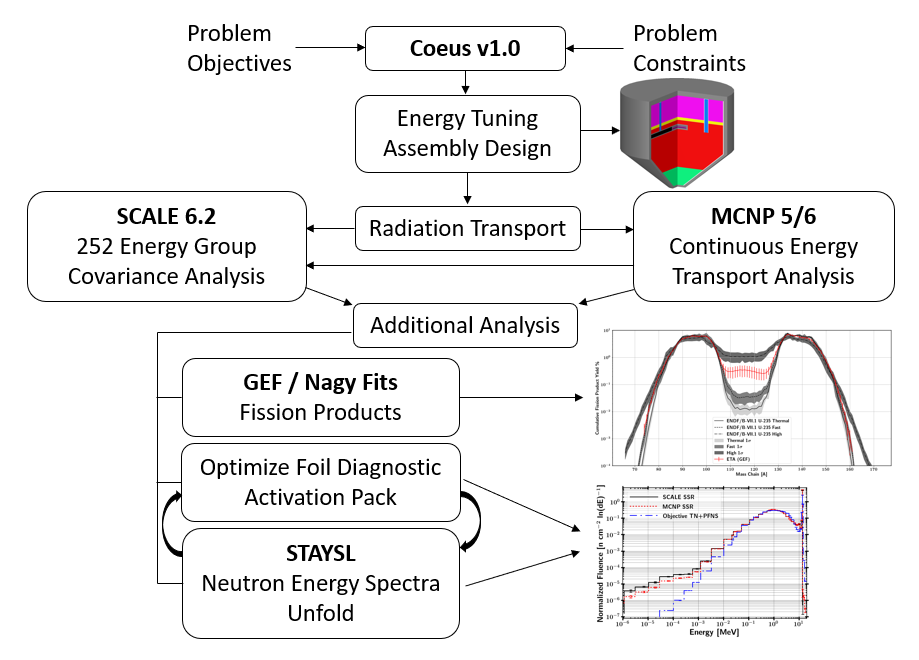
\includegraphics[width=\linewidth]{Figures/Chapter3/ETA_Flow.png}
	\caption{Overview of the major research components from ETA design to key analysis areas.}
	\label{fig:ETAFLOW}
\end{figure}

\section{Energy Tuning Assembly Design}

\ The ETA analyzed in this research was taken as an initial condition; however, it is important to understand the motivation that went into the design. 
Each of the objectives and constraints have impacts on the ability of ETA to effectively shape the neutron source to a TN+PFNS.  

\ The TN+PFNS was created utilizing the Godiva bare critical assembly, a metallic sphere of HEU, to approximate the down-scattered components from the TN and PFNS source neutrons. 
A Watt fission spectrum volume source and a 14.1 MeV centered point source at a 10 keV plasma temperature were transported through Godiva using MCNP6 \cite{Bevins, MCNP6}. 
The Godiva transmitted components combined to generate the TN+PFNS with 15\% fusion born neutrons and 85\% Watt fission neutrons.  
The objective spectrum was created with the 46 group DPLUS structure, which is utilized in radiation shielding problems and in the DABL69 library \cite{Bevins, ADVANTG}. 

\subsection{NIF Constraints}

There were a few limits imposed by NIF that do not directly affect the analysis performed in this study but did affect the ETA design, spectral shaping capability, and fission product production. 
The three main constraints were a weight limit, stay-out angle, and distance from the DT source, all of which are linked together to form the experimental geometric envelope available for the designed ETA. 

The first constraint was a maximum weight of 75 kg. 
The weight limit lowers the ability of ETA to match the objective spectrum by decreasing the scope of design possibilities and mass available to modify the spectrum. 
The weight constraint was derived based on the limits of the diagnostic and instrument manipulator (DIM) planned to field ETA at the NIF. 
The closest standoff range was 15 cm from the DT source mounted on the target positioner (TARPOS) given the allowable weight. 
Finally, the stay-out angle provides the laser paths a clear line of sight from the beam ports to the DT capsule. 
A diagram of the planned ETA experiment is shown in Figure \ref{fig:exp}.
Since the original design, the experiment has been moved to target and diagnostic manipulator (TANDM) 90-124, which provides opportunities to re-evaluate the overall constraints due to increase lift capacity.

\begin{figure}[hbt!]
	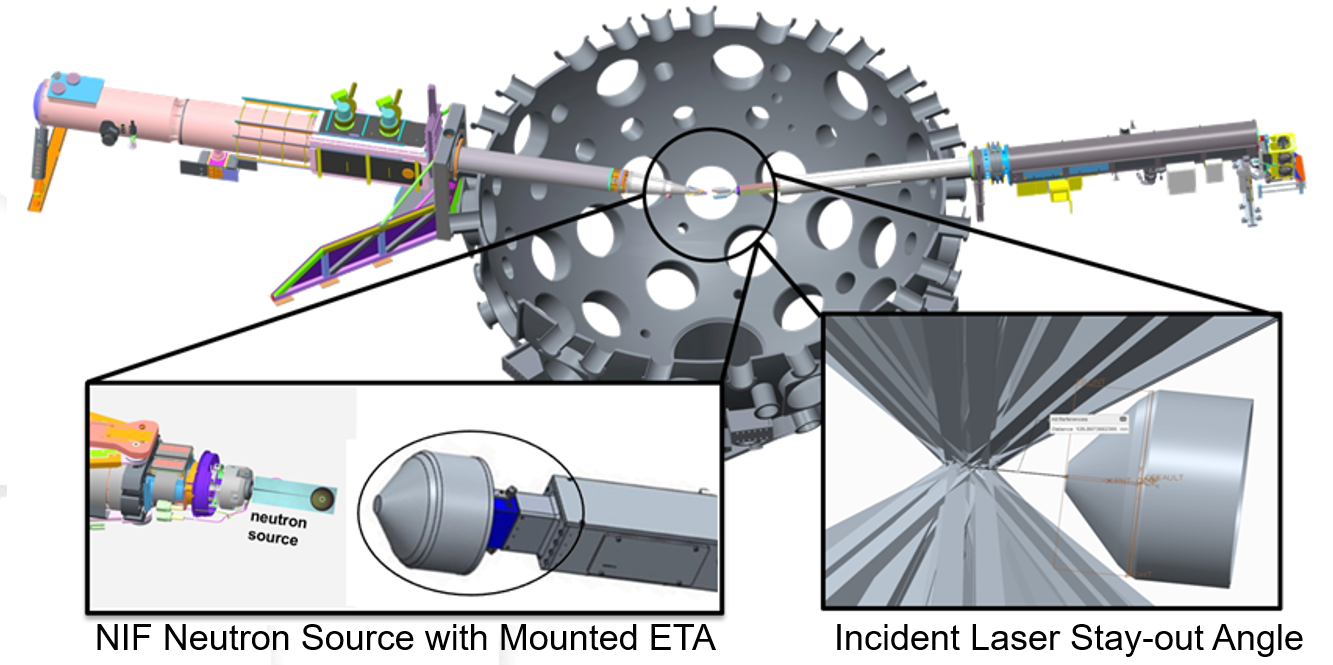
\includegraphics[width=\linewidth]{Figures/Chapter3/Experimental_Setup.png}
	\caption[Diagram of ETA experiment at the NIF showing ETA installed on TANDM 90-124 with neutron source mounted on TARPOS 90-239.]{Diagram of ETA experiment at the NIF showing ETA installed on TANDM 90-124 with neutron source mounted on TARPOS 90-239. The bottom left graphic shows a notional mounting of ETA on TANDM 90-124. The bottom right graphic highlights the laser path clearance requirement constraint.}
	\label{fig:exp}
\end{figure}

\subsection{NIF Source}

\ The NIF source neutron spectrum used in the original design of ETA was a ``high foot" shot at the NIF and is shown in Figure \ref{fig:NIFSRC3}.
The indirect drive ``high foot" source utilized a hohlraum, shown in Figure \ref{fig:NIFSRC4}, whic is responsible for the large downscattered source component shown in Figure \ref{fig:NIFSRC3} \cite{NIF1}.  

\begin{figure}[htb!]
	\centering
	\includegraphics[width=13cm]{Figures/Chapter3/SRC_Obj_leth.png}
	\caption{Comparison of objective TN+PFNS to NIF source constraint utilizing the 140520 NIF shot.}
	\label{fig:NIFSRC3}
\end{figure}

\begin{figure}[htb!]
	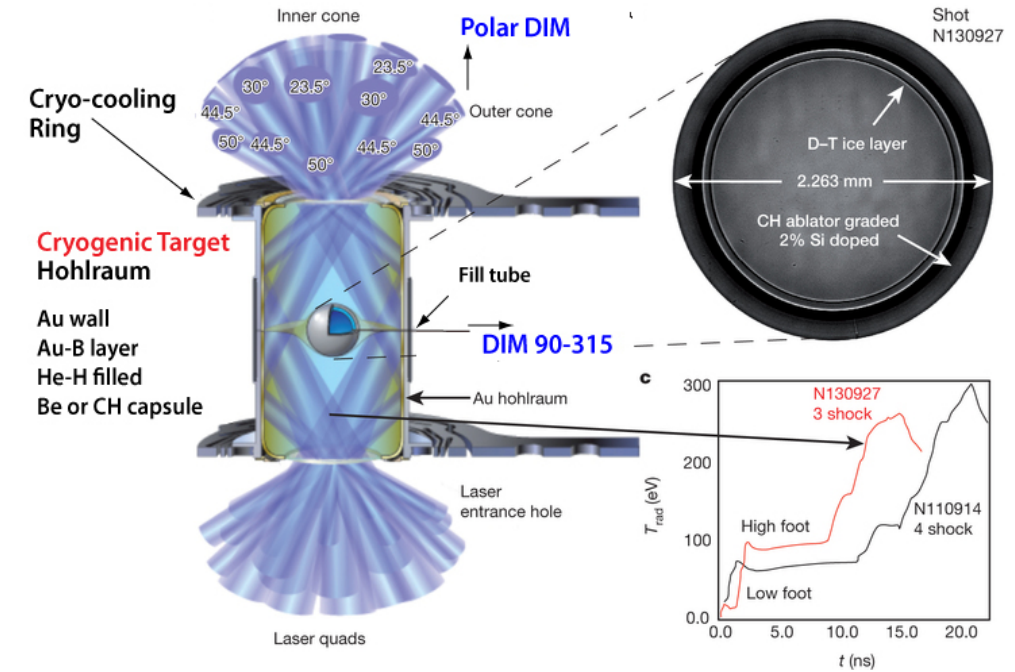
\includegraphics[width=\linewidth]{Figures/Chapter3/Hohlraum.png}
	\caption[NIF shot N130927 utilizing a hohlraum and image of DT source.]{NIF shot N130927 utilizing a hohlraum and image of DT source \cite{NIF1}}. 
	\label{fig:NIFSRC4}
\end{figure}

\ However, source development is a continuing process, and direct drive sources with high neutron outputs and a reduced downscattering component have been developed. 
The current NIF source modeled for this work was a DT Polar Drive Exploding Pusher (PDXP) target with a nominal yield of \num{3.7e+15} neutrons from laser-driven inertial confinement fusion. 
The PDXP source is a DT mixture (65:35 ratio DT) compressed to 8 atmospheres \cite{Yeamans2017a}. 
The capsule is comprised of a hydrocarbon glow discharge polymer (GDP) 2.9 mm in diameter \cite{Chen2017}. 
The PDXP source does not utilize auxiliary systems to achieve compression, unlike other NIF sources that require a hohlraum to smooth out the ablation surface. 
Instead the compression is driven solely by the NIF laser configuration. 
The large benefit of using a low-mass target is the removal of downscattering within the source hohlraum. 
This has enabled the PDXP source to be modeled as a 14 MeV point source in previous NIF experiments. 
The plasma burn width is approximatley 300 ps, so all of the neutrons were modeled as being emitted instantaneously \cite{Yeamans2017a}.

\ Many experimental models at NIF utilize a zero-temperature plasma value for the neutron source because the inertial confinement process is not at equilibrium, making any temperature value an indirect measurement. 
These models often use DT neutrons modeled as a 14.03 MeV isotropic point source.
However, this is an approximation that neglects the spread in neutron energies due to the plasma temperature.

\ The plasma temperature from the fusion reaction will result in a distribution of neutron energies due to differences in reaction rates and imparted energy from conservation of mass and energy \cite{Brysk1973}. 
The distribution of neutron energies produced by the NIF is taken as a theoretical thermal plasma at a temperature of 10.75 keV \cite{Appelbe2014}. 
The resultant Gaussian distribution centered at 14.06 MeV has a full width at half maximum of approximately 0.58 MeV. 
The unnormalized source probability distribution function for the input spectrum based on the plasma temperature approach is shown in Figure \ref{fig:NIFSRC1}. 

\begin{figure}[htb!]
	\includegraphics[width=13cm]{Figures/Chapter3/Applebe1075keV.png}
	\caption{10.75 keV plasma temperature DT fusion neutron energy distribution.}
	\label{fig:NIFSRC1}
\end{figure}

\section{Radiation Transport}

\ Three radiation transport simulations were performed to analyze ETA. 
Both MCNP5 and the MAVRIC sequence in SCALE were utilized to increase the degree of confidence in the results. 
The radiation transport simulations provided results for the reaction rates for foil activation, neutron energy spectra, and temporal aspect of the neutron flux.
The modeling efforts and purpose of each code are described in the sections that follow. 

\subsection{Nuclear Data Libraries}\label{libraries}

\ Different nuclear data libraries were utilized depending on the application and code system. A summary of the nuclear data libraries utilized in this work is shown in Table \ref{table:libs}. 

\begin{table}[htb!]
	\centering
	%\tiny
	\setlength\extrarowheight{2.5pt}
	\caption{Summary of nuclear data libraries utilized for MCNP, MAVRIC, and Sampler simulations. }
	\label{table:libs}
	\begin{tabular}{|l|l|l|}
		\hline
\multicolumn{1}{|c|}{Monte Carlo Code} & \multicolumn{1}{c|}{Transport} & \multicolumn{1}{c|}{Reactions} \\ \hline
MCNP5 & ENDF/B-VII.1 & \begin{tabular}[c]{@{}l@{}}IRDFF v.1.05                    \\ Binned into STAYSL 129 group \\ and DPLUS 46 group\end{tabular} \\ \hline
SCALE MAVRIC & ENDF/B-VII.1 & IRDFF v.1.05 \\ \hline
SCALE Sampler & ENDF/B-VII.1 252 group & \begin{tabular}[c]{@{}l@{}}ENDF/B-VII.1 252 group             \\ IRDFF v.1.05 252 group\\ Collapsed to 66 group\end{tabular} \\ \hline
	\end{tabular}
\end{table}

First, the continuous energy neutron transport simulations performed in MCNP and SCALE utilized the ENDF/B-VII.1 library\cite{ENDF}. 
ENDF is a comprehensive nuclear library that contains the data necessary for the transport calculation. 
ENDF/B-VII.1 was also used for response functions not available in IRDFF or where the IRDFF data was consistent with ENDF. 
The multi-group nuclear data transport calculations were performed with the 252 group SCALE library based on ENDF/B-VII.1 \cite{SCALE}. 
The 252 group structure is the largest fidelity multi-group SCALE library with samples distributed to utilize in Sampler.
The activation foil reactions largely utilized the IRDFF v.1.05 library \cite{IRDFF}. 

\ It is commonplace for nuclear data libraries to have equivalent information when drawing from the same experimental sources or from each other directly; however, differences do arise in the evaluated data as highlighted in Figure \ref{fig:aung}. 
While there is good agreement among the data libraries in the $\mathrm{^{197}}$Au (n,g) uncertainty, IRDFF had a much larger uncertainty from 1 to 4 keV, and the SCALE 252 group library drops to zero uncertainty after approximately 2.5 MeV. 
Some of the deviations were based on the group structure utilized. 

\begin{figure}[hbt!]
	\centering
	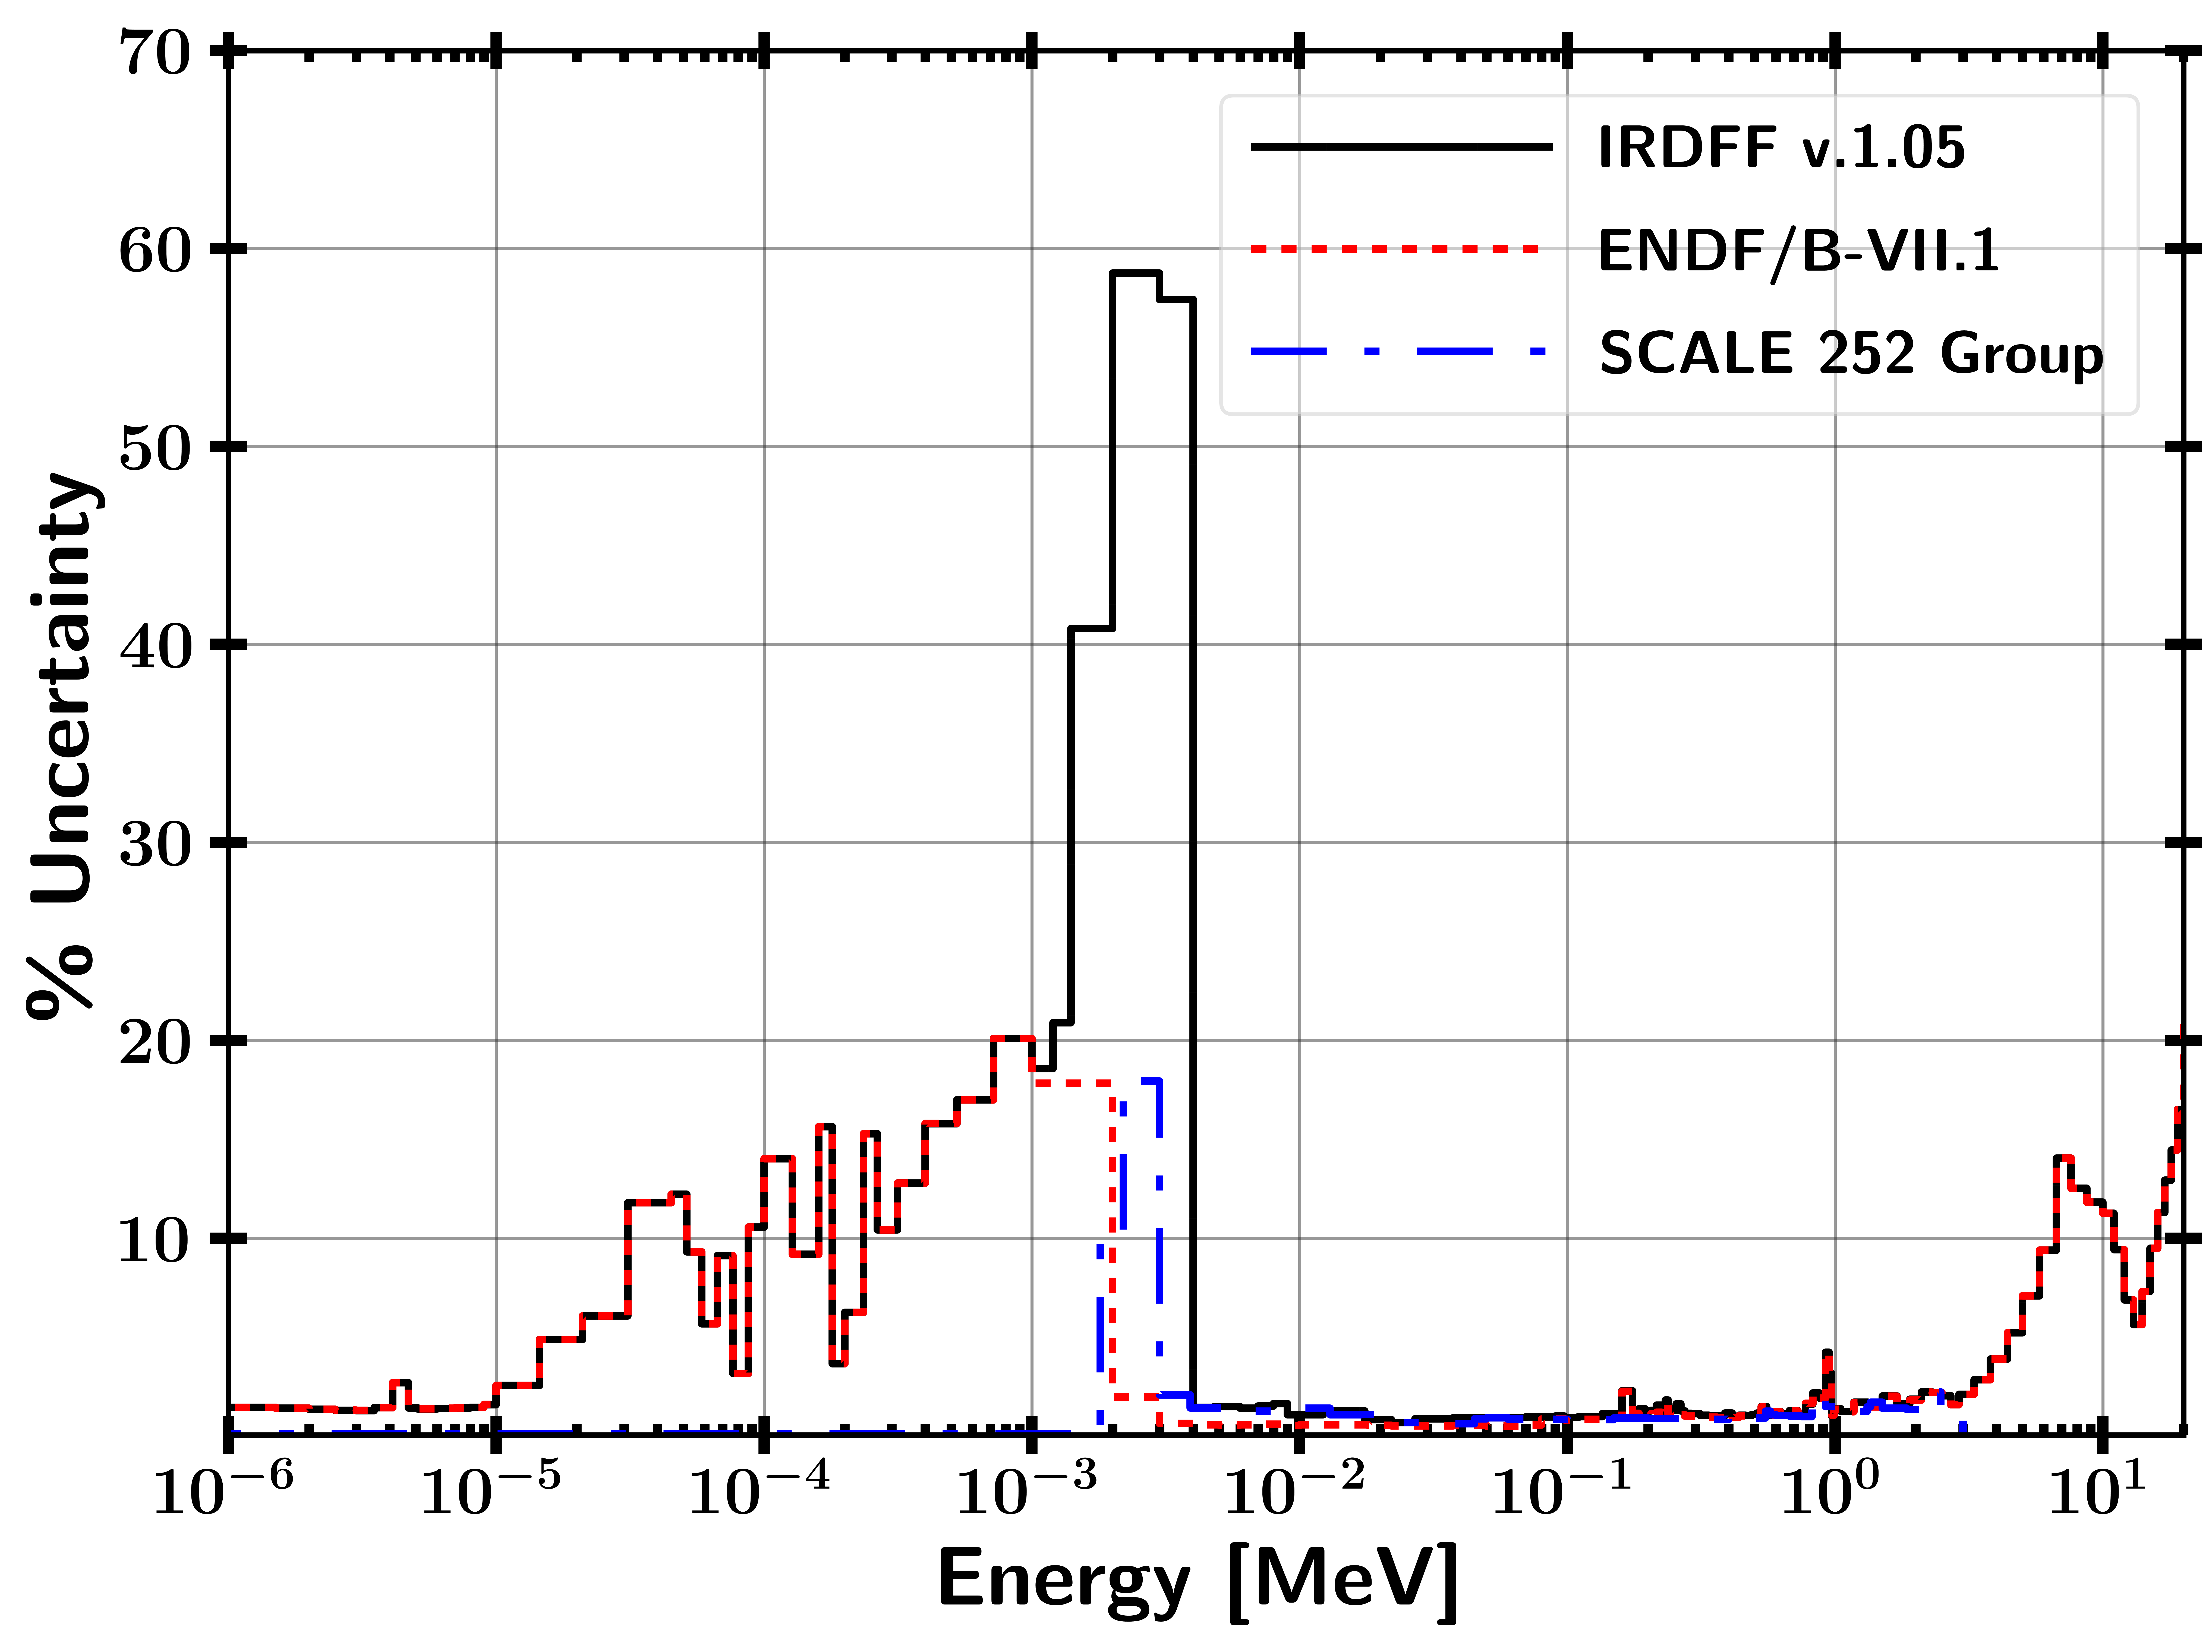
\includegraphics[width=13cm]{Figures/Chapter3/Au_ng_Uncertainty.png}
	\caption[Comparison between IRDFF v.1.05, ENDF/B-VII.1, and SCALE 252 Group ENDF/B-VII.1 $\mathrm{^{197}}$Au (n,g) reaction cross-section uncertainties.]{Comparison between IRDFF v.1.05, ENDF/B-VII.1, and SCALE 252 Group ENDF/B-VII.1 $\mathbf{^{197}}$Au (n,g) reaction cross-section uncertainties.}
	\label{fig:aung}
\end{figure}

A few reactions utilized the SCALE ENDF data when the SCALE 252 group data was consistent with the IRDFF or data was not available in the IRDFF. 
The activation foils and tallied reactions that did not use the IRDFF were $\mathrm{^{55}}$Mn (n,g), U  (n,f), and $\mathrm{^{186}}$W (n,g). 
A comparison between the uncertainties for $\mathrm{^{55}Mn} (n,g)$ is shown in Figure \ref{fig:mnng}. 
Overall, there was agreement between the uncertainties. 
The energy region where the uncertainty has been truncated encompasses a negligible percentage of the reactions, so the effect is minimal. 

\begin{figure}[hbt!]
	\includegraphics[width=13cm]{Figures/Chapter3/Mn_ng_Uncertainty.png}
	\caption[Comparison between IRDFF v.1.05, ENDF/B-VII.1, and SCALE 252 Group ENDF/B-VII.1 $\mathrm{^{55}}$Mn (n,g) reaction cross-section uncertainties.]{Comparison between IRDFF v.1.05, ENDF/B-VII.1, and SCALE 252 Group ENDF/B-VII.1 $\mathbf{^{55}}$Mn (n,g) reaction cross-section uncertainties.}
	\label{fig:mnng}
\end{figure}

\subsection{MCNP}

\ A continuous energy radiation transport simulation was performed in MCNP5 in collaboration with LLNL  \cite{MCNP5}. 
The NIF model in MCNP5 has been utilized for numerous experiments and moving from MCNP to other radiation transport codes is cumbersome due to the high fidelity geometric model that has been built. 
ETA was modeled in the full NIF chamber including TARPOS 90-239, TANDM 90-124 with mounted ETA, TANDM 90-348 with diagnostics, the polar DIM, and the first panel walls \cite{NIF_Overview2}. 
The ancillary equipment and surroundings were incorporated into the model to account for neutron `room return' in the NIF chamber.
The mean flux at the HEU sample, expected activities of foils, and fission numbers were determined using $2\times10^{11}$ source particles. 

The variance reduction techniques utilized were importance cells and the SSR.
The importance cells split the weight of particles crossing into a region of different importance. This allows for a higher number of particles to be in the region of interest which has high importance. 
Conversely, neutrons in area of low importance can be removed from the system. Neutrons in low importance regions have a low probability of contributing to the tallies of interest, so it is not computationally efficient to track them. 

The SSR was created with ETA and the NIF to account for the radiation transport up to surfaces in the simulation. The particles that cross the surfaces are tracked to be used as a starting source for additional simulations that accounts for the behavior of the model outside of the surfaces. The particle energy, weight, position, and direction are maintained which eliminates computational time for simulations that are in the same geometric configuration. 
The MCNP SSR file was used to create sources representing the incident flux from the DT source and room return from supporting equipment.
The SSR surfaces were a disk 17.5 cm in diameter at the front (source facing) and bottom of ETA and a connecting cylinder as shown in Figure \ref{fig:sursource}. 

\begin{figure}[hbt!]
	\centering
	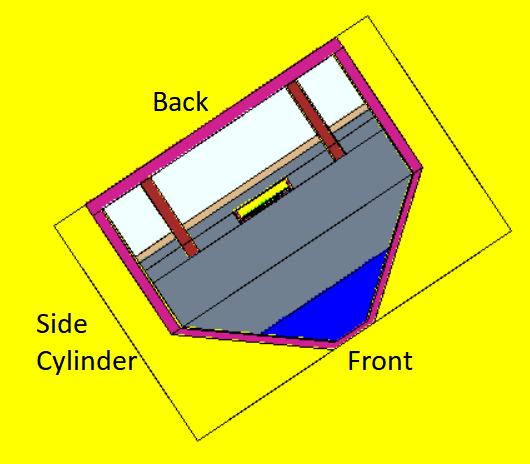
\includegraphics[width=9cm]{Figures/Chapter3/SurfacesSSR.png}
	\caption[Surfaces for NIF source SSR file.]{Surfaces for NIF source SSR file. The front source faced the DT point source and the back surface was mounted to TANDM 90-124.}
	\label{fig:sursource}
\end{figure}

The normalized probability distribution functions for the source locations are shown in Figure \ref{fig:RSSASpec}. 
The effect of the room return in the NIF chamber is most clearly shown in the cylindrical and back surface.  
The front-facing surface also contains room return; however, the source 14.03 MeV neutrons dominated the spectrum. 

\begin{figure}[htb!]
	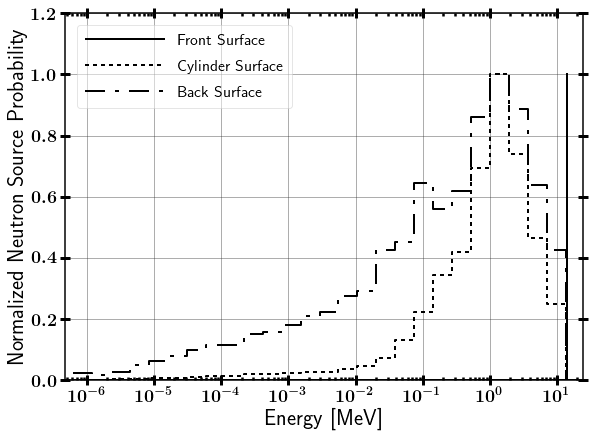
\includegraphics[width=\linewidth]{Figures/Chapter3/RSSA_Spectrum.png}
	\caption{Surfaces source probability distribution functions mapped to SCALE.}
	\label{fig:RSSASpec}
\end{figure}

The MCNP5 results were used to benchmark the continuous energy solution in MAVRIC. 
Although it was not feasible to perfectly replicate the source distribution because there are many scattering angles crossing a surface in different directions, it was possible to approximate the behavior for the purpose of quantifying the effect of nuclear data covariance. 

\subsection{MAVRIC}\label{Benchmark}
\ A continuous energy radiation transport simulation was performed in the MAVRIC software framework which utilizes automated variance reduction techniques along with a traditional Monte Carlo transport calculation. 
The three SSR sources were mapped over to SCALE by approximating the behavior with source definitions. 
The total fluence of neutrons passing through the front, back, and cylindrical SSR surfaces were $6.5\times10^{14}$, $3.5\times10^{12}$, and $2.4\times10^{12}$, respectively. 
The front source was approximated as a point with the strength determined from the spherical divergence ($1/R^{2}$) of the source neutrons to the front facing surface.  
The back source was a disk, and the cylinder was four equal strength line sources facing ETA and emitting in 2$\pi$. 
Ideally, the cylindrical source could be mapped over with a cylindrical source; however, the reference directions for emission in SCALE are in Cartesian coordinates. 

The benchmarking of the mapping of MCNP to SCALE was performed by comparing the reactions in the foil pack and neutron flux in the HEU foil. 
A comparison between MCNP and MAVRIC reactions products in the foils and fissions is summarized in Table \ref{table:act_sum}. 
Two key aspects were important to determining a goodness of fit. 
First, the magnitude of the reaction difference between the continuous MCNP and MAVRIC reactions was the primary measure.
Second, there is not a systematic pattern to the differences between the threshold or thermal reactions modeled in SCALE and MCNP. 


\begin{table}[htb!]
\centering
	%\tiny
	\setlength\extrarowheight{2.5pt}
	\caption[Activation foil reactions comparison between continuous energy MCNP SSR and MAVRIC mapped SSR.]{Activation foil reactions comparison between continuous energy MCNP SSR and MAVRIC mapped SSR. All statisitcal uncertainties were below 0.2\%. }
	\label{table:act_sum}
\begin{tabular}{|c|c|c|c|}
\hline
\multirow{2}{*}{Reaction} & \begin{tabular}[c]{@{}c@{}}MCNP SSR \\ Continuous Energy\end{tabular} & \multicolumn{2}{c|}{\begin{tabular}[c]{@{}c@{}} MAVRIC\\   Continuous Energy\end{tabular}} \\ \cline{2-4} 
& Reactions & Reactions & \begin{tabular}[c]{@{}c@{}}Percent Change\\  Relative to MCNP\end{tabular} \\ \hline
$\mathrm{^{90}Zr}$ (n,2n) $\mathrm{^{89}Zr}$ & 1.89E+09 & 1.91E+09 & 1.5 \\ \hline
$\mathrm{^{58}Ni}$ (n,2n) $\mathrm{^{57}Ni}$ & 1.87E+08 & 1.90E+08 & 1.4 \\ \hline
$\mathrm{^{58}Ni}$ (n,p) $\mathrm{^{58}Co}$ & 6.54E+09 & 6.64E+09 & 1.5 \\ \hline
$\mathrm{^{197}Au}$ (n,2n) $\mathrm{^{196}Au}$ & 2.91E+09 & 2.91E+09 & -0.1 \\ \hline
$\mathrm{^{197}Au}$ (n,g) $\mathrm{^{198}Au}$ & 1.00E+09 & 1.02E+09 & 2.0 \\ \hline
$\mathrm{^{115}In}$ (n,n') $\mathrm{^{115}In^{m1}}$ & 3.81E+09 & 3.82E+09 & 0.05 \\ \hline
$\mathrm{^{115}In}$ (n,g) $\mathrm{^{116}In^{m1}}$ & 5.14E+09 & 5.19E+09 & 1.0 \\ \hline
$\mathrm{^{27}Al}$ (n,a) $\mathrm{^{24}Na}$ & 1.08E+09 & 1.08E+09 & -0.02 \\ \hline
$\mathrm{^{186}W}$ (n,g) $\mathrm{^{187}W}$ & 7.21E+08 & 7.30E+08 & 1.2 \\ \hline
$\mathrm{^{55}Mn}$ (n,g) $\mathrm{^{56}Mn}$ & 3.14E+08 & 3.23E+08 & 2.8 \\ \hline
$\mathrm{^{235}U} (n,f)$ & 1.94E+09 & 1.96E+09 & 0.5 \\ \hline
$\mathrm{^{238}U} (n,f)$ & 2.70E+07 & 2.67E+07 & -1.1 \\ \hline
Total Fissions & 1.99E+09 & 2.00E+09 & 0.5 \\ \hline
	\end{tabular}
\end{table}

\ The continuous energy SCALE reactions matched fairly well to the MCNP reactions. 
There was a noted bias of approximately 1\% for increasing the number of reactions in the continuous energy MAVRIC simulation; however, these are within the differences documented in Section \ref{'secMC'}. 
Nonetheless, there were some key deficiencies in the way that the sources were mapped. 
First, the SSR source had $10^{9}$ sample written points. 
In MCNP, these points re-sampled at the same entry location on the SSR with new random numbers. 
For SCALE, the SSR was homogenized over the surfaces. 
Also, there was a systematic bias of the room return that was not captured in the source approximations. 
The ancillary equipment in the room increased the scattering back to ETA. 
Again, this was homoginized over the source surfaces in the SCALE simulations. 
The angular resolution for the SCALE line and disk sources were restricted to equal probability in 2$\pi$. 
% Dr. Petrosky recommended removing this too. I think Bevins said it was not needed either. Removing. 
%\ Figures \ref{fig:logflux1} and \ref{fig:linflux1} show the relative residual flux on a logarithmic and linear energy scale comparing the MCNP values to the SCALE continuous energy MAVRIC and SCALE 252 group Sampler values. 
%There are three regions of differences between the continuous energy solutions; the 252 group comparison is described in the next section. 
%First, no tallies were captured in SCALE above 14.2 MeV. 
%These events born from HEU fissions were very low probability and do not contribute largely to the result. 
%Second, there is a slight difference between 10 MeV and the prompt DT peak which is likely caused by the systematic room return that was homogenized.
%Last, at low energy ($<$ 1 keV) there was a larger thermal flux than the MCNP flux which can be attributed to the approximations in source mapping. 

%\begin{figure}[hbt!]
%	\centering
%	\includegraphics[width=15cm]{Figures/Chapter3/Residuals.png}
%	\caption[Logarithmic energy fluence residuals comparing MCNP, SCALE MAVRIC Continuous Energy (CE), and SCALE 252 group Sampler.]{Logarithmic energy fluence residuals comparing MCNP, SCALE MAVRIC Continuous Energy (CE), and SCALE 252 group Sampler. The relative residuals tally compared to MCNP values of 0, 1, and -1 indicate agreement, double the flux was tallied and all of the flux was not tallied, respectively.}
%	\label{fig:logflux1}
%\end{figure}

%\begin{figure}[hbt!]	
%	\centering
%	\includegraphics[width=15cm]{Figures/Chapter3/Residuals_lin.png}
%	\caption[Linear energy fluence residuals comparing MCNP, SCALE MAVRIC Continuous Energy (CE), and SCALE 252 group Sampler.]{Linear energy fluence residuals comparing MCNP, SCALE MAVRIC Continuous Energy (CE), and SCALE 252 group Sampler. The relative residuals tally compared to MCNP values of 0, 1, and -1 indicate agreement, double the flux was tallied and all of the flux was not tallied, respectively.}
%	\label{fig:linflux1}
%\end{figure}

\subsection{SCALE Sampler Sequence}\label{'secSCALEMG'}

\ A 252 group radiation transport simulation was performed for 182 discrete trials in Sampler to build a distribution of Monte Carlo responses to capture the systematic nuclear data uncertainty. 
The Sampler sequence is a ``super-sequence" that acts as a wrapper above the MAVRIC sequence \cite{SCALE}. 
The nuclear data libraries were randomly perturbed to determine the distribution of responses due to uncertainty in the transport due to nuclear data.  

The SCALE Sampler module enabled analysis of nuclear data covariance. 
The unperturbed nuclear data was executed for the first sample along with a user-defined number of samples. 
The sample nuclear data libraries are perturbed nuclear data based on the covariance  largely developed from ENDF/B-VII.1; however, additional information is included from ENDF/B-VI, ENDF/B-VII.2 (proposed at the time), JENDL-4.0, and collaborative research between Brookhaven National Laboratory, Los Alamos National Laboratory, and Oak Ridge National Laboratory.
Finally, the nuclear data covariance libraries included information completed in the Working Party on International Nuclear Data Evaluation Cooperation Subgroup-26 \cite{SCALE}.

\ The associated Sampler libraries contained 1,000 pre-sampled neutron cross-sections limited to 56 and 252 group structures. 
It is important to note the weighting functions for SCALE's library which are a Maxwellian from 10$^{-5}$ eV to 0.1 eV, a Watt fission spectrum from 80 keV to 10 MeV, and $1/E$ between 0.1 eV to 80 keV and for 10 to 20 MeV.  
A notable issue with utilizing a single group structure for all applications is the weighting function to process the continuous energy cross-sections will impact results if the flux is dramatically different. 
This problem is difficult in that a group structure would be needed for each individual problem and is further complicated by changes in the neutron spectra in different regions of a problem. 

\ The continuous energy MAVRIC script was modified by changing the library to the 252 group version and adding the Sampler wrapper to maintain the same inputs. 
Table \ref{table:act_sum1} presents a comparison between MCNP and SCALE MAVRIC 252 group reactions products in the foils and fissions.
There are some important discrepancies that are caused by the 252 group structure. 
The 252 group Sampler mean total reactions were generally in agreement with the continuous energy solutions with three exceptions: $\mathrm{^{89}}$Zr, $\mathrm{^{57}}$Ni, and $\mathrm{^{56}}$Mn. 
The impact of these differences is outlined in Section \ref{Mapping}.
The first two threshold reactions were attributed directly to the flux weighting of the 13.8 to 14.6 MeV group utilized in the energy region where the reaction occured. 
The 252 group $\mathrm{^{55}}$Mn reaction difference from MCNP was caused by the flux weighting used to create the group cross-section, and the bulk of the difference occurs below 80 keV.   
The 252 group library performed well for the majority of the reactions because many of the activation reactions are saturated by the PFNS, which is synonymous with the Watt Fission neutron spectrum. 

\begin{table}[htb!]
	\centering
	%\tiny
	\setlength\extrarowheight{2.5pt}
	\caption[Activation foil reactions comparison between continuous energy MCNP SSR and 252 group MAVRIC mapped SSR.]{Activation foil reactions comparison between continuous energy MCNP SSR and 252 group MAVRIC mapped SSR. All statisitcal uncertainties were below 0.2\%. }
	\label{table:act_sum1}
	\begin{tabular}{|c|c|c|c|}
\hline
\multirow{2}{*}{Reaction} & \begin{tabular}[c]{@{}c@{}}MCNP SSR \\ 252 Group \end{tabular} & \multicolumn{2}{c|}{\begin{tabular}[c]{@{}c@{}} MAVRIC\\   252 Group\end{tabular}} \\ \cline{2-4} 
& Reactions & Reactions & \begin{tabular}[c]{@{}c@{}}Percent Change\\  Relative to MCNP\end{tabular} \\ \hline
$\mathrm{^{90}Zr}$ (n,2n) $\mathrm{^{89}Zr}$ & 1.89E+09 & 2.05E+09 & 8.6 \\ \hline
$\mathrm{^{58}Ni}$ (n,2n) $\mathrm{^{57}Ni}$ & 1.87E+08 & 2.20E+08 & 17.4 \\ \hline
$\mathrm{^{58}Ni}$ (n,p) $\mathrm{^{58}Co}$ & 6.54E+09 & 6.65E+09 & 1.5 \\ \hline
$\mathrm{^{197}Au}$ (n,2n) $\mathrm{^{196}Au}$ & 2.91E+09 & 2.93E+09 & 0.6 \\ \hline
$\mathrm{^{197}Au}$ (n,g) $\mathrm{^{198}Au}$ & 1.00E+09 & 9.92E+08 & -0.8 \\ \hline
$\mathrm{^{115}In}$ (n,n') $\mathrm{^{115}In^{m1}}$ & 3.81E+09 & 3.86E+09 & 1.2 \\ \hline
$\mathrm{^{115}In}$ (n,g) $\mathrm{^{116}In^{m1}}$ & 5.14E+09 & 5.14E+09 & -0.1 \\ \hline
$\mathrm{^{27}Al}$ (n,a) $\mathrm{^{24}Na}$ & 1.08E+09 & 1.06E+09 & -1.1 \\ \hline
$\mathrm{^{186}W}$ (n,g) $\mathrm{^{187}W}$ & 7.21E+08 & 7.09E+08 & -1.8 \\ \hline
$\mathrm{^{55}Mn}$ (n,g) $\mathrm{^{56}Mn}$ & 3.14E+08 & 2.64E+08 & -15.9 \\ \hline
$\mathrm{^{235}U} (n,f)$ & 1.94E+09 & 1.95E+09 & 0.01 \\ \hline
$\mathrm{^{238}U} (n,f)$ & 2.70E+07 & 2.70E+07 & 0.03 \\ \hline
Total Fissions & 1.99E+09 & 1.99E+09 & 0.004 \\ \hline	
	\end{tabular}
\end{table}


%\ Additionally, from Figures \ref{fig:logflux1} and \ref{fig:linflux1}, there were notable differences in the multi-group modeled neutron flux spectrum compared to the continuous energy results. 
%First, the neutron population between 10 and 14 MeV was increased as the macroscopic cross-sections for Bi and W are overestimated in the group-wise cross-section. 
%While here was similar behavior to the continuous energy solution at low energy, the multi-group approach was also slightly increased compared to MCNP due to the increased reactions at high energy. 

\ Sampler was performed for 182 trials until the responses converged to a solution to build the distribution of responses to use for random sampling and bootstrapping. 
Figure \ref{fig:Convergence1} displays the convergence of the mean and uncertainty of the bootstrapped values for a few selected reactions. 
The $\mathrm{^{55}}$Mn (n,g) was the least converged and largest relative error reaction due to high systematic uncertainty and relatively large nuclear data uncertainty over the energy range of the ETA spectrum. 

Bootstrapping is a method to determine uncertainty in a given dataset by using random sampling with replacement.
The bootstrapped values are equivalent to a Gaussian distribution if the underlying data is Gaussian in shape. 
However, bootstrapping is most useful if a distribution of responses does not follow a Gaussian distribution.
The results of each of the perturbed nuclear data samples were combined using statistical bootstrapping.

SCALE's functionality can automatically perform some of this work; however, the addition of IRDFF covariance to the responses made it necessary to develop a set of Python 2.7 functions to process the data. 
First, a sample is randomly selected from the $n$ samples in the dataset. 
The ``0" sample contained the unperturbed nuclear data result, while the 1 through n samples used perturbed nuclear data. 
Next, the 252-group energy structure was collapsed into a 66 group structure to reduce statistical uncertainty, $\sigma_{stat}$, in the lower energy bins.  

Finally, the value and the relative uncertainty associated with the response is used to sample from a Gaussian distribution to include the statistical error from that trial. 
The process was repeated 10,000 times, with replacement to provide $<$ 0.1\% convergence of the relative error of the bootstrapped value. 
The final value and relative uncertainty are used as the final result, which includes $\sigma_{stat}$ and systematic uncertainty, $\sigma_{sys}$.

\begin{figure}[hbt!]	
	\centering
	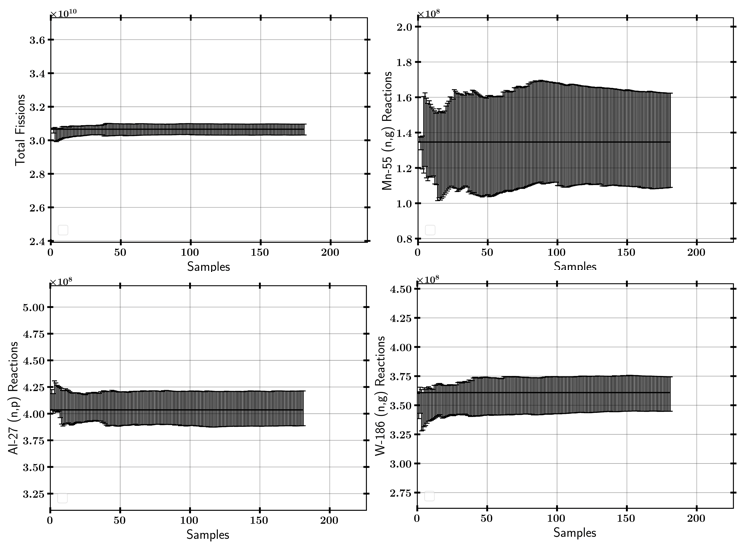
\includegraphics[width=15cm]{Figures/Chapter3/Convergence1.png}
	\caption[U(n,f), $\mathrm{^{55}}$Mn (n,g),  $\mathrm{^{27}}$Al (n,p), and  $\mathrm{^{186}}$W (n,g) sampled histogram and reaction convergence as a function of Sampler trial.]{U(n,f), $\mathbf{^{55}}$Mn (n,g),  $\mathbf{^{27}}$Al (n,p), and  $\mathbf{^{186}}$W (n,g) sampled histogram and reaction convergence as a function of Sampler trial. The convergence graphs included the IRDFF nuclear data covariance.}
	\label{fig:Convergence1}
\end{figure}

\section{Nuclear Data Covariance}\label{Multi}

Capturing the full nuclear data uncertainty is essential because it is often a dominant unknown in nuclear applications \cite{Campolina2018}. 
The majority of uncertainty analyses done to date focus on integrated quantities such as the effective criticality of a nuclear reactor \cite{Rochman2016}\cite{Griseri2017}.
However, applications such as radionuclide production rely on a single reaction channel that is observed, which can have much larger uncertainties than noted in integral quantities.
Furthermore, it is important to note that ENDF-based uncertainties may also be underestimates of the general nuclear data uncertainty \cite{Bostelmann2017}. 

\ The methodology to incorporate the IRDFF nuclear data in the SCALE Sampler module is shown in Figure \ref{fig:method1}. 
There are three key contributions to the uncertainty of a result in this radiation transport simulation. 
First, the uncertainty in the neutron transport was quantified using the SCALE Sampler module. 
Second, the uncertainty in the reaction cross-section was assessed using IRDFF data. 
In most uncertainty quantification analysis, these two nuclear data $\sigma_{sys}$ are treated at the same time.
However, they are separated in this analysis to incorporate the IRDFF reactions and uncertainty. 
Last, every Monte Carlo-based result has $\sigma_{stat}$, which can be driven to negligible values with sufficient computational resources. 

\begin{figure}[htb!]
	\centering
	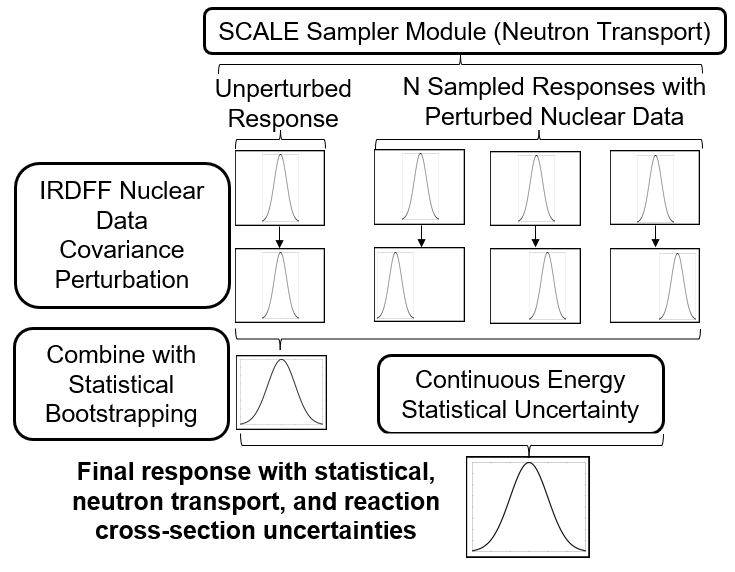
\includegraphics[width=11cm]{Figures/Chapter3/Method.png}
	\caption{Methodology flowchart to insert nuclear data uncertainty for reaction channel from alternative library into SCALE.}
	\label{fig:method1}
\end{figure}

%Then, each of the independent samples from Sampler were modified according to the IRDFF nuclear data covariance information separately from the perturbation data in SCALE. 
%In some cases noted in Section \ref{libraries}, such as $\mathrm{^{55}}$Mn (n,g), ENDF data was utilized because it was consistent with IRDFF thereby avoiding the separate modification\cite{ENDF}. 
%For each trial, the sample reactions were correlated through an equivalent neutron flux, but the reaction cross-sections are independently varied. 
%The resultant responses were combined using statistical bootstrapping as the final response distribution was assumed to be non-Normally distributed. 
%Finally, some applications required a group structure different than what is available in Sampler which can be accomplished with a continuous energy neutron transport calculation. 
%The Sampler $\sigma_{stat}$ was replaced by the continuous energy $\sigma_{stat}$ assuming $\sigma_{sys}$ and $\sigma_{stat}$ were added in quadrature. 
% Why was this all commented?

\subsection{Sampling Transport Related Uncertainties}

\ The SCALE Sampler module was utilized to assess the neutron transport response uncertainty by generating independent samples to characterize the distribution of responses.
The transport-related uncertainties are quantified in the neutron fluence on the HEU and activation foils. 
For each trial, Sampler utilized a different set of $\sigma_{rxn}$ to transport the source neutrons through the geometry. 
The variance in the energy-dependent fluence over the trials determined the transport related uncertainties. 
One benefit of the 252 group structure utilized by SCALE was that the uncertainty in the reaction rates follows linearly from the fluence, so better statistics at low energy are easier to achieve in comparison with the continuous energy solution. 

\subsection{Sampling Nuclear Data Covariance Libraries}

\ Sampler can perturb additional variables; however, there are presently no methods to include correlations to allow a user-defined response function in Sampler (i.e. IRDFF cross-section) to be sampled with a covariance matrix.   
Instead the reaction rate response was calculated independently of the Sampler runs assuming that the nuclear data followed a correlated multivariate normal distribution utilized by the SCALE Sampler sequence \cite{Wieselquist2013, Zhu2015, Williams2013, SCALE}. 
The nuclear cross-sections were converted to a 252 group format in SCALE, while the uncertainties were converted from the IRDFF format by linear interpolation of the midpoint bin energies. 
The linear interpolation was used to approximate the uncertainty when the bin structure did not align with the mapped energy group structure, which was deemed appropriate due to the linear variation in the uncertainty over small energy ranges. 
% Alternatives to this approach include processing with NJOY or assuming a flux weighted ratio of uncertainties to create a new bin uncertainty. 

\ The nuclear data and uncertainty were sampled from the multivariate normal distribution for each independent Sampler trial. 
The reaction tally ($R$) result was perturbed by the ratio of the macroscopic cross-sections ($\Sigma$) before and after multivariate random sampling to create group-wise perturbation parameters ($Q$) with the neutron flux ($\phi$) over 252 groups (g). 

\begin{equation} \label{eq:LeastSq1}
R\  =\ \sum_{g=1}^{252} \ \phi_{g}  \ \Sigma_{g} \ Q_{g}
\end{equation} 

\noindent The net result effectively modified the microscopic cross-section to form the perturbed $R$. 
The multivariate normal distribution sampled data acted as a set of constants that are multiplied to each energy group  \cite{Williams2013}. 
%% I thought each sample had an indpendent flux, that flux was then colved with M samples of IRDFF reaction data, and this process was repeated for each of the N samples so that you had NxM reaction rates. No, I just did it on the N samples, so I did not reuse fluxes. 
 
%The sampled reaction trails were combined with statistical bootstrapping where random samples were drawn with replacement of the trial values and corresponding statistical uncertainty to determine the mean and standard deviation. 
% I think this last sentence can be removed and is covered in the next section?


\subsection{The Case for Sampling with Alternative Probability Distribution Functions}
\ Common practice for stochastic sampling approaches are built around the multivariate normal distribution, which is a straightforward way to sample nuclear data covariance matrices. 
However, the log-normal distribution is more appropriate for physical properties that cannot have negative values such as neutron cross-sections which can have uncertainties greater that 100\% \cite{Zerovnik2013}. 
The log-normal distribution and normal distribution produce similar approximations for small relative uncertainties, but the distributions diverge significantly for large uncertainties. 
For example, the $\mathrm{^{55}}$Mn (n,g) reaction has large uncertainty at high neutron energies. 
The evaluated cross-section and experimental data informing the (n,g) reaction cross-section near 14 MeV in ENDF/B-VII.1 is shown in Fig. \ref{fig:Mn}. 

\begin{figure}[htb!]
	\includegraphics[width=\linewidth]{Figures/Chapter3/Mn_Eval.png}
	\caption{Experimental nuclear data informing $\mathrm{^{55}}$Mn (n,g) reaction in comparison with the evaluated nuclear data contained in ENDF/B-VII.1 \cite{ENDF}.}
	\label{fig:Mn}
\end{figure}

The experimental data is spread over an order of magnitude, but it is most dense around the evaluated cross-section, thereby supporting the use of a log-normal distribution over the normal distribution. 
The sampling of the nuclear data covariance matrices assuming a log-normal distribution instead of  a normal distribution can produce drastically different results in radiation transport simulations. 

To illustrate why a log-normal or similar distribution may be more appropriate, a Monte Carlo simulation was conducted simulating darts thrown at a board with a mean value in the x and y Cartesian coordinates of 0.5. 
This example assumes negative values are a non-physical quantity.
Three distributions were compared over varying uncertainty: a normal distribution, a normal distribution with negative numbers rejected as is done with the multivariate normal distribution approach, and a log-normal distribution\footnote{The SCALE Sampler sequence utilizes a multivariate normal distribution with negative numbers rejected and reassigned.}. 
The mean dart position and mean radius were compared, and the outcome is shown in Table \ref{table:MCDarts}. 
The distribution of darts is shown in \mbox{Figure \ref{fig:darts}}. 

\begin{figure}[!htbp]
	\centering
	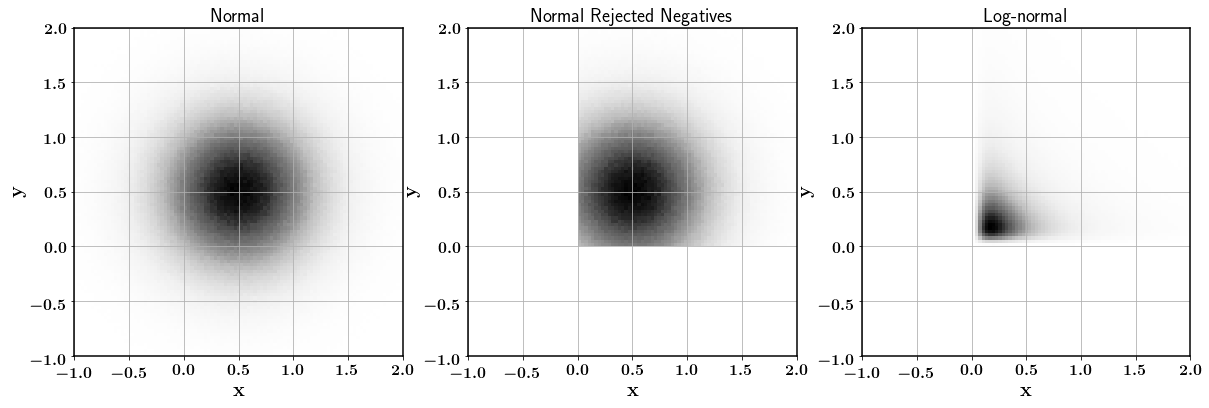
\includegraphics[width=\linewidth]{Figures/Chapter3/Normal.png}
	\caption{Normal, normal with rejected negatives, and log-normal distribution of darts in example Monte Carlo simulation with a mean value of 0.5 in the x and y Cartesian directions and an position uncertainty of 100\% in each direction.}
	\label{fig:darts}
\end{figure}
% These feel like they could fit side-by-side.  I also think having the x and y axes fixed for each would make the comparison easier

\begin{table}[htb!]
	\setlength\extrarowheight{2.5pt}
	\centering
	\caption{Monte Carlo Darts results with normal, normal with rejected negative values, and log-normal distributions.}
	\label{table:MCDarts}
	\begin{tabular}{|c|c|c|c|}
		\hline
		Distribution & Normal & Normal Rejected & Log-normal \\ \hline
		\multicolumn{4}{|c|}{$\mu$ = 0.5 $\sigma$ = 0.5} \\ \hline
		$\bar{x}$ and $\bar{y}$ & 0.5 $\pm$ 0.5 & 0.64 $\pm$ 0.4 & 0.5 $\pm$ 0.5 \\ \hline
		$\bar{r}$ & 0.63 $\pm$ 0.32 & 0.50 $\pm$ 0.25 & 0.51 $\pm$ 0.49 \\ \hline
		\multicolumn{4}{|c|}{$\mu$ = 0.5 $\sigma$ = 0.25} \\ \hline
		$\bar{x}$ and $\bar{y}$ & 0.5 $\pm$ 0.25 & 0.51 $\pm$ 0.24 & 0.5 $\pm$ 0.25 \\ \hline
		$\bar{r}$ & 0.31 $\pm$ 0.16 & 0.29 $\pm$ 0.15 & 0.29 $\pm$ 0.19 \\ \hline
		\multicolumn{4}{|c|}{$\mu$ = 0.5 $\sigma$ = 0.05} \\ \hline
		$\bar{x}$ and $\bar{y}$ & 0.5 $\pm$ 0.05 & 0.5 $\pm$ 0.05 & 0.5 $\pm$ 0.05 \\ \hline
		$\bar{r}$ & 0.06 $\pm$ 0.03 & 0.06 $\pm$ 0.03 & 0.06 $\pm$ 0.03 \\ \hline
	\end{tabular}
\end{table}

\ There were important aspects of the outcomes of this simplistic example. 
First, all distributions performed well at low uncertainty, which was expected given that a log-normal and normal distribution are close approximations in this range. 
This shows that a normal distribution is a good approximation for stochastic sampling radiation transport codes for materials with low relative uncertainties. 
At large uncertainty, where negative values are drawn often, there were many differences that affect the results of sampling. 
The normal and log-normal distributions predicted the mean Cartesian coordinate values well.
However, the range of radii from the points were different as the underlying distributions behaved differently at large uncertainty as the log-normal distribution most probable value is lower value but had a larger likelihood of sampling relatively large numbers. 
The negative value removed normal distribution overestimated the mean value as more emphasis was placed on the larger numbers.
Manipulations could have been made to weight lesser valued non-negative samples to create a better fitting solution; however, this would still not be completely representative of the normal distribution. 
Ultimately, sampling from a normal distribution was not the optimal solution when the uncertainty in the data was large. 
The neutron transport uncertainties and sampling method are fortunately somewhat mitigated because uncertainties are generally larger in regions where the reaction cross-section is lower, so the net result on the problem may be reduced. 

The methodology for sampling the nuclear data libraries utilized the multivariate normal distribution to stay consistent with Sampler and the other versions of stochastic sampling methods noted. 
The uncertainties of the reaction cross-sections utilized by the IRDFF are below 10\%, so the impact of utilizing the multivariate normal distribution instead of one more closely following the physics is minimal. 
It is important to understand the implications of utilizing each sampling method. 
The effect to this research is that the true nuclear data uncertainty may not be fully achievable, but rather an estimation of the uncertainty is determined.
However, it is essential to note that there is no inherent uncertainty to nuclear data \cite{SCALE}. 
Instead the uncertainties and correlations are an evaluation based on experimental data and models and not always a true quantification of the uncertainty. 
Furthermore, stochastic sampling uncertainty quantification techniques allows for an estimation of the uncertainty consistent with published evaluated data.

% Very cool analysis!  It would seem that the issues should be relatively small since even 50% uncertainty produces the same(ish) results.  Is there a formal justification for using the multivaraiate normal distro in the literatiure? 
% Not that I have seen. I have mostly found people saying that we should use the log-normal when uncertainty is large. 

%\subsection{Statistical Bootstrapping of Sampler Results}

%\ The results of each of the perturbed nuclear data samples were combined using statistical bootstrapping.
%Bootstrapping is a method to determine uncertainty in a given dataset by using random sampling with replacement.
%The bootstrapped values are equivalent to a Gaussian distribution if the underlying data is Gaussian in shape. 
%However, bootstrapping is most useful to use here if a distribution of responses does not follow a Gaussian distribution.

%SCALE's functionality can automatically perform some of this work; however, the addition of IRDFF covariance to the responses made it necessary to develop a set of Python 2.7 functions to process the data. 
%First, a sample is randomly selected from the $n$ samples in the dataset. 
%The ``0" sample contained the unperturbed nuclear data result, while the 1 through n samples have perturbed nuclear data. 
%Next, the 252-group energy structure was collapsed into a smaller group size to reduce $\sigma_{stat}$ uncertainty in the lower energy bins. 
%Finally, the value and the relative uncertainty associated with the response were used to sample from a Gaussian distribution to include the statistical error from that trial. 
% Not quite following this previous sentence - better?
%The process was repeated to 10,000 times, with replacement to provide under 0.1\% convergence of the bootstrapped value relative error. 
%The final value and relative uncertainty are used as the final result, which includes $\sigma_{stat}$ and  $\sigma_{sys}$.

%Several Python 2.7 functions were built to parse and perform bootstrapping on the SAMPLER outputs.
% the use of SAMPLER vs Sampler is inconsistent throughout; I think the sentence should be removed, but I wanted to make that point. They are also inconsistent in the Manual. I thought I caught all of these. 

\subsection{Mapping Nuclear Data Systematic Error to Alternate Group Structures}\label{Mapping}
% I might be tired, but I didn't follow this section easily.

One important approximation that must be made for group-wise cross-section uncertainty models is that the uncertainty is not largely dependent on the group-structure. 
A study performed by Wieselquist \textit{et al.} benchmarking nuclear data uncertainty between two methods showed that the integral uncertainty is relatively insensitive to the group structure utilized \cite{Wieselquist2013}. 
% However, it should be noted that the integrated and the differential uncertainty both play an important role in the results but need to be handled slightly differently.
% I modified this sentence, but it isn't completely clear to me what the point is here. The point was to introduce that I will be talking about both below. 
Additionally, there is uncertainty in published uncertainties making any small differences found between alternate group structures potentially negligible.  

\ A test case for the $\mathrm{^{58}}$Ni (n,2n) reaction was performed to outline the impact of the weighting function and group structure on the uncertainty results. 
The $\mathrm{^{58}}$Ni (n,2n) reaction in ENDF was linear in energy and in cross-section which enabled straightforward analytical solutions. 
The cross-sections from ENDF/B-VII.1 available in SCALE are shown in Figure \ref{fig:nixs} along with the relative uncertainty of the reaction cross-section used by SCALE. 
% The 252 group cross-section was slightly weighted to lower energies in this energy range. 
% \subsubsection{Case Study}
\ The test case utilized a normalized flux integral of 1 $n-cm^{-2}-s^{-1}$ from the threshold energy of 12.4 MeV up to 20 MeV with the flux bin weighted by the bin widths. 
The flux profile was chosen to eliminate bias from the energy bin shapes for the 252 group structure. 
The test flux is shown in Figure \ref{fig:testflux}.

\begin{figure}[!htb]
	\centering
	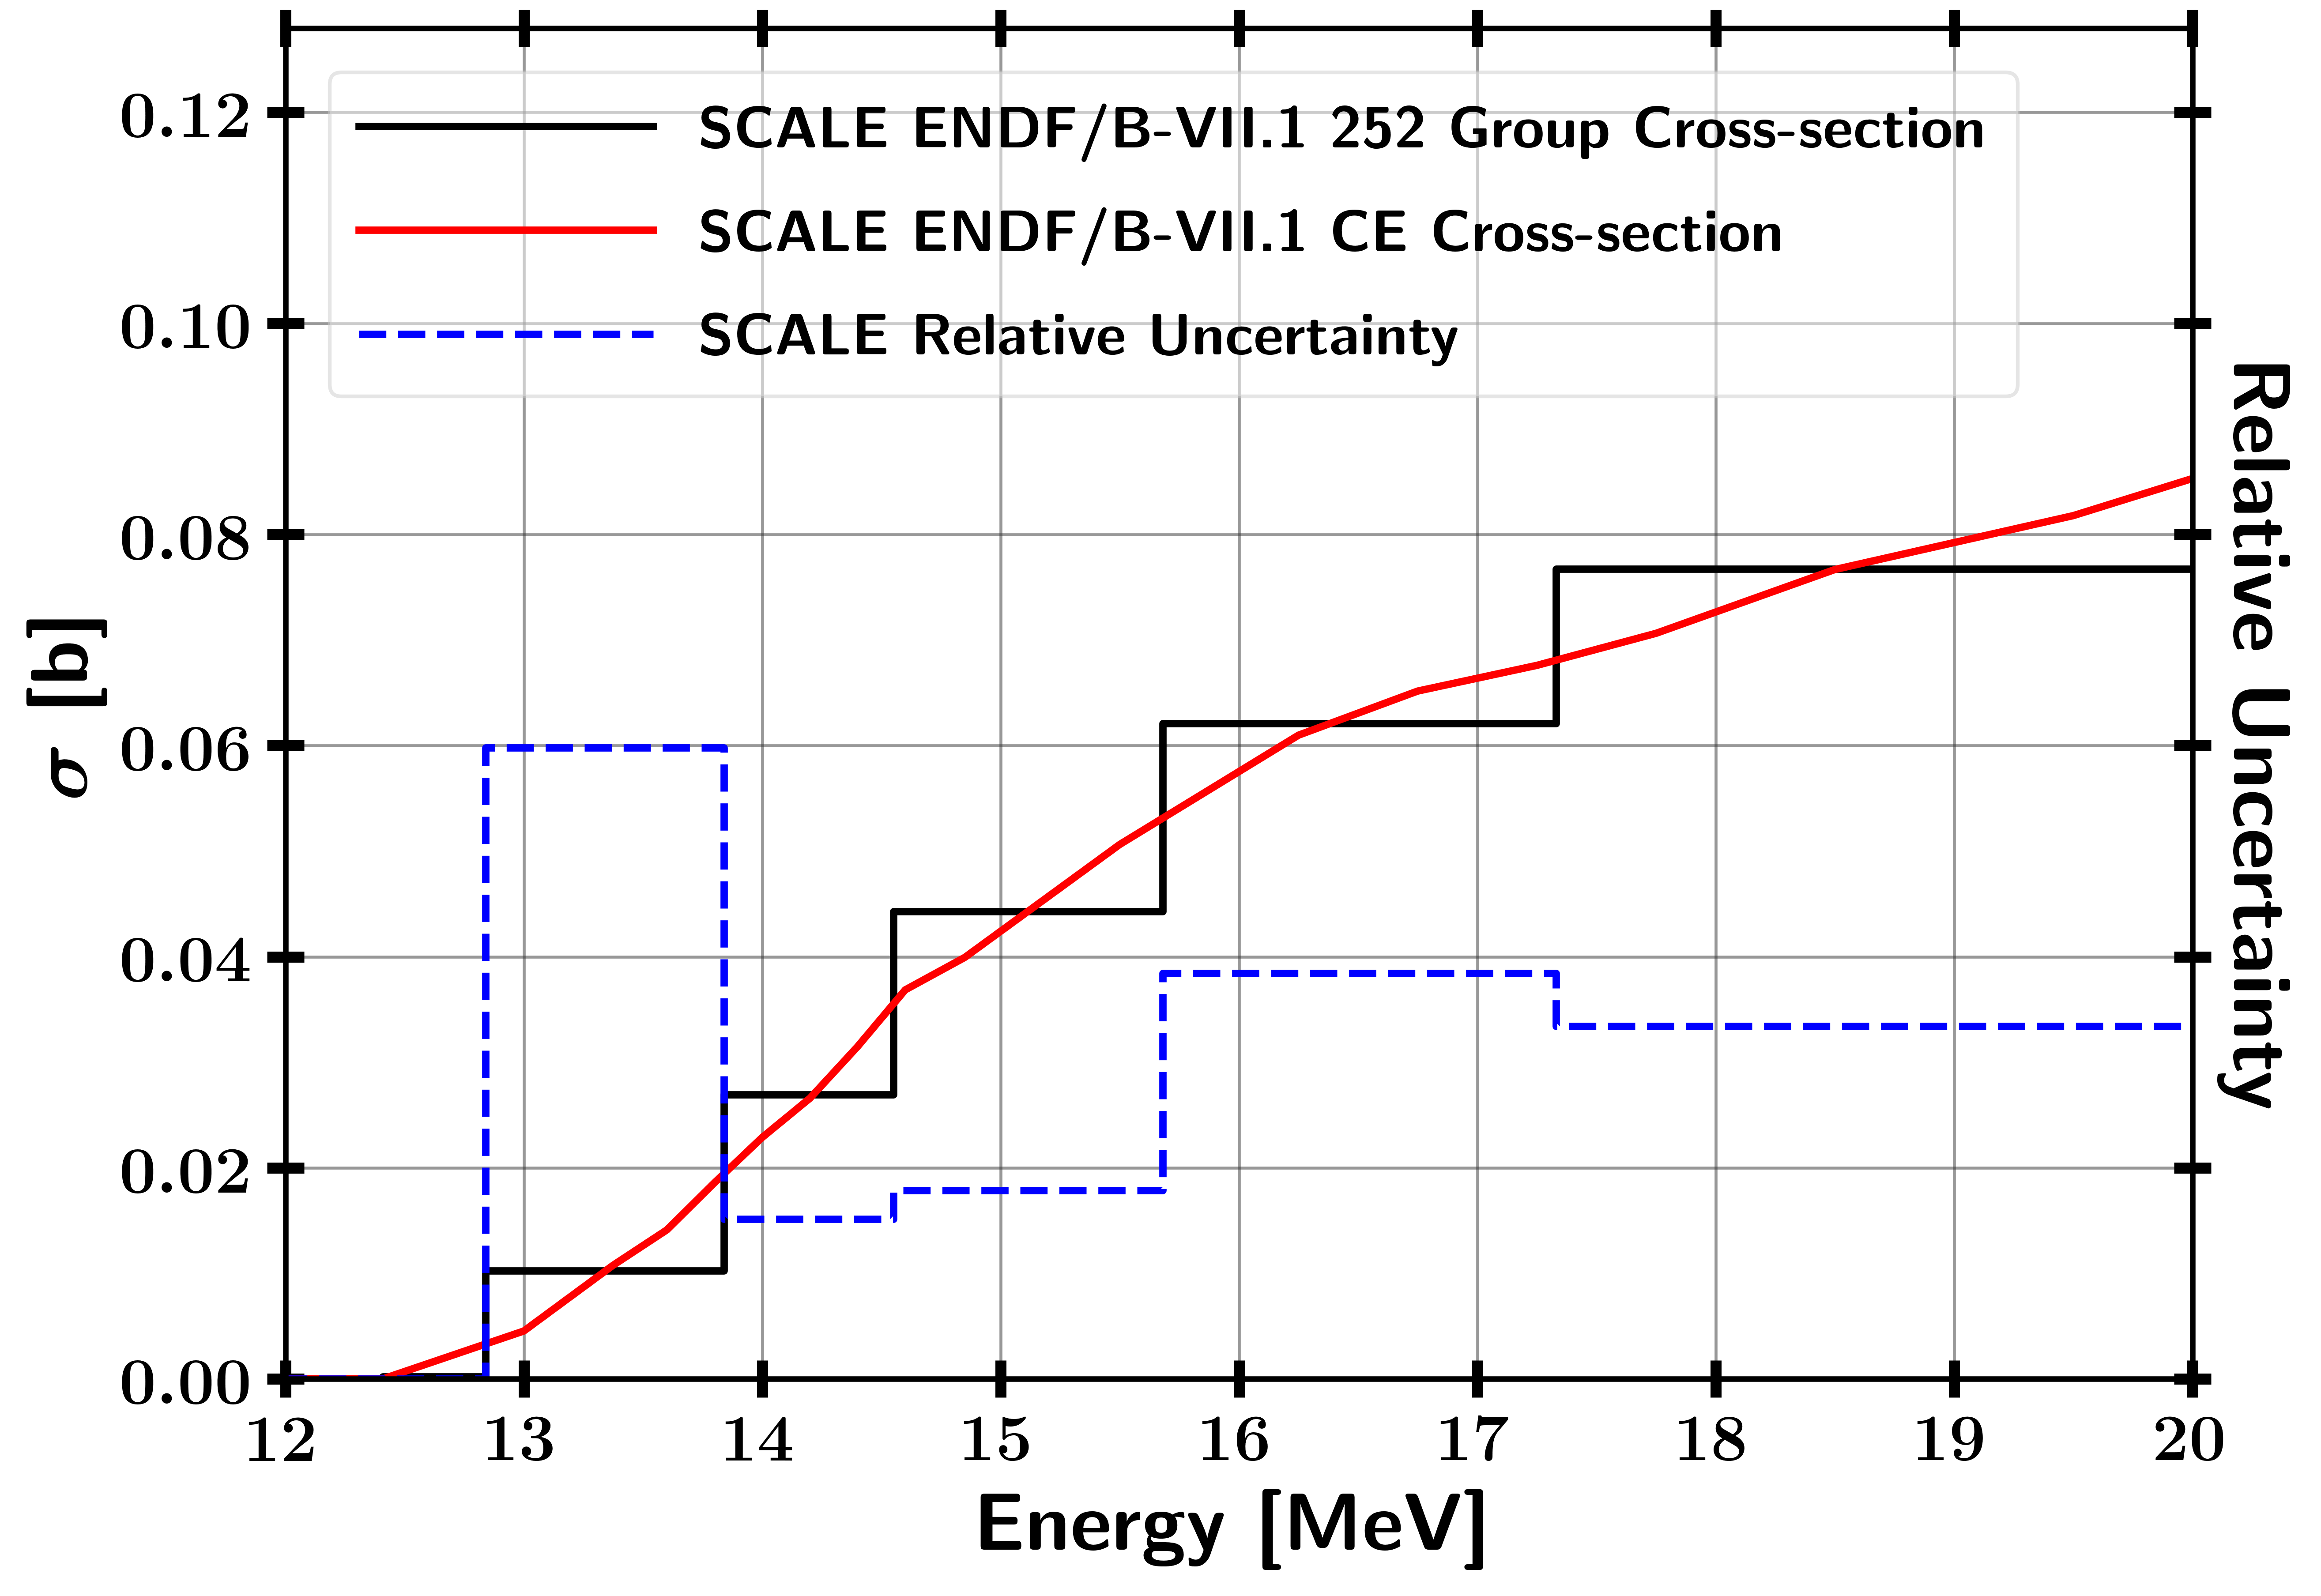
\includegraphics[width=13cm]{Figures/Chapter3/nin2n_b_u.png}
	\caption[Comparison between $\mathrm{^{58}Ni}$ (n,2n) continuous energy (CE) and 252 group $\mathrm{1/E}$ weighted cross-sections. The relative uncertainty of the reaction cross-section is shown.]{Comparison between $\mathbf{^{58}Ni}$ (n,2n) continuous energy (CE) and 252 group $\mathbf{1/E}$ weighted cross-sections. The relative uncertainty of the reaction cross-section is shown.}
	\label{fig:nixs}
\end{figure}

\begin{figure}[!htb]
	\centering	
	\includegraphics[width=13cm]{Figures/Chapter3/example_Flux.png}
	\caption{$\mathbf{^{58}Ni}$ (n,2n) case study constant differential flux.}
	\label{fig:testflux}
\end{figure}

\ The reaction rate for the continuous energy cross-section resulted in 0.005117 $\pm$ 3.255\% reactions per  $cm^{3}-s^{1}$, while the 252 group structure cross-section resulted in 0.005095 $\pm$ 3.244\% reactions per  $cm^{3}-s^{1}$. The 252 group structure underestimated $R$ compared to the continuous energy solution by 0.4\% for the test case.  
More importantly, the reaction uncertainty differed by 0.2\%, which means uncertainties may differ from the continuous energy solution by approximately the same magnitude as $R$. Although, a flux could possibly be created to skew this much further. 
This conclusion presents the issue of determining the uncertainties when the group structure produces results that are significantly different. 
The implication for this research means that the reaction uncertainty can only be determined up the error introduced by the 252 group nuclear data library. 
% $\mathrm{^{89}}$Zr, $\mathrm{^{57}}$Ni, and $\mathrm{^{56}}$Mn reaction uncertainties can vary by approximately 10-20\% of their nominal value.  
% Is this conclusion a problem since some of the R values have a no insignificant difference? Yes :(
\subsubsection{Integral Data}

\ The total reaction uncertainty was determined by the uncertainty in the bootstrapped 252 group value. 
The integral uncertainty was used with the mean value from the continuous energy solution. 
It is important to note that the uncertainty in this uncertainty is on the order by which the group-wise transport analysis misrepresents the continuous energy solution based on the previous section. 

\subsubsection{Differential Data}
\ The differential uncertainties were treated as being a function of energy through linear interpolation of the midpoint bin energies. 
This approach provided an approximation of the total uncertainty for the target bin structures. 
The 252 group structure results were a quadrature combination of $\sigma_{stat}$ and  $\sigma_{sys}$ which follows from the error propagation. 
The 252 groups were collapsed at low energy to create a 66 group structure.  

\begin{equation} \label{eq:uncertainty}
\sigma_{total}  \ = \ \sqrt{\sigma_{sys}^{2} \ + \sigma_{stat}^{2}}
\end{equation} 

\noindent Thereby $\sigma_{sys}$ was determined for each group. 
The reverse treatment was performed to add in $\sigma_{sys}$ to the target group structure. 

\section{Activation Foil Pack and Neutron Energy Spectrum Unfolding}

\subsection{Activation Foils Selection}

Vagena, \textit{et al.} concluded that Au, As, Cd, In, Ir, Er, Mn, Ni, Se, Sm, W, and Zn were suitable to fully cover the neutron energy spectrum ranging from 0.01 eV to 18 MeV which is also of interest to the TN+PFNS \cite{Vagena2018b}.
In addition to this identified set, the modeled ETA experiment at NIF had a large amount of high energy neutron flux necessitating the use of additional high energy foils.  
Unfortunately, the experimental cavity in the ETA did not have enough space to fit all of these foils.

\ The foil pack designed to be placed in the ETA experimental cavity was created to be able to successfully unfold the incident neutron spectrum using the activation foil data. 
The activation foils were selected using many important criteria including the cross-section, gamma emission, and half-life as discussed in Section \ref{FoilsHere}.
However, the most notable aspects were the confidence in the nuclear data, the inclusion of the isotope reaction in the IRDFF database, and energy range in which the foils experience activation.   

\ The final set of foils, containing Zr, Ni, Au, In, Al, W, and Mn, was analyzed for this study. 
Geometric constraints allowed for approximately 7 mm thickness of the foils to be placed in the sample cavity.
All of the foils suggested could not fit in the ETA sample cavity and increasing the number of foils would decrease the amount of reactions in the foils, thereby decreasing the foil activity for unfolding techniques.  
The thickness of the foils was chosen to be 1 mm because that is a standard foil thickness at the NIF.
All foils were modeled with a radius of 2.5 cm aside from Au and Al which were 2 cm that is normally utilized at the NIF.
The foils chosen have activations over a large portion of the ETA neutron spectrum. 
Zn was replaced by Al because the Al (n,a) reaction is in the IRDFF v.1.05, and the reaction cross-sections are nearly equivalent in shape.
Additionally, Zr-90 (n,2n) was added to provide more high energy neutron detection which is a very large component of the ETA spectrum. 
The relevant nuclear data and foil thicknesses for each selected foil are summarized in Table \ref{table:foils111}. 

\begin{table}[htb!]
	\centering
	\caption{Activation foils selected for ETA experiment to be utilized to unfold the neutron energy spectrum. Each reaction has well documented nuclear data and is available within the IRDFF utilized by STAYSL.}
	\label{table:foils111}
	\setlength\extrarowheight{2.5pt}
	\resizebox{\textwidth}{!}{%
		\begin{tabular}{|c|c|c|c|c|}
			\hline
			Foil (Thickness) & Reaction & \begin{tabular}[c]{@{}c@{}}Threshold {[}MeV{]} \\ (@ 10 mb)\end{tabular} & \begin{tabular}[c]{@{}c@{}}Decay Radiation \\ {[}keV{]} (Intensity)\end{tabular} & $t_{1/2}$ \\ \hline
			Zr (1 mm) & $\mathrm{^{90}Zr}$ (n,2n) $\mathrm{^{89}Zr}$ & 12.1 (12.1) & 909.2 (0.9904) & 78.41 hrs \\ \hline
			\multirow{2}{*}{Ni (1 mm)} & $\mathrm{^{58}Ni}$ (n,2n) $\mathrm{^{57}Ni}$ & 12.4 (13.3) & 1,378 (0.817) & 35.6 hrs \\ \cline{2-5} 
			& $\mathrm{^{58}Ni}$ (n,p) $\mathrm{^{58}Co}$ & 0 (1.3) & 810.8 (0.9945) & 70.86 days \\ \hline
			\multirow{2}{*}{Au (0.1 mm)} & $\mathrm{^{197}Au}$ (n,2n) $\mathrm{^{196}Au}$ & 8.1 (8.3) & 355.7 (0.87) & 6.17 days \\ \cline{2-5} 
			& $\mathrm{^{197}Au}$ (n,g) $\mathrm{^{198}Au}$ & Thermal & 411.8 (0.9562) & 2.69 days \\ \hline
			\multirow{2}{*}{In (1 mm)} & $\mathrm{^{115}In}$ (n,n') $\mathrm{^{115}In^{m1}}$ & 0.336 (0.597) & 336.24 (0.459) & 4.49 hrs \\ \cline{2-5} 
			& $\mathrm{^{115}In}$ (n,g) $\mathrm{^{116}In^{m1}}$ & Thermal & 1293.56 (0.848) & 54.29 min \\ \hline
			Al (1 mm) & $\mathrm{^{27}Al}$ (n,a) $\mathrm{^{24}Na}$ & 3.25 (6.7) & 1368.63 (0.9999) & 15 hrs \\ \hline
			W (1 mm) & $\mathrm{^{186}W}$ (n,g) $\mathrm{^{187}W}$ & Thermal & 685.51 (0.332) & 24 hrs \\ \hline
			Mn (1 mm) & $\mathrm{^{55}Mn}$ (n,g) $\mathrm{^{56}Mn}$ & Thermal & 846.8 (0.9885) & 2.58 hrs \\ \hline
		\end{tabular}%
	}
\end{table}

% I'm torn whether to include this list below; it is good information but not necessarily needed.  
% I thought it was good to show why they were disculded. I know a lot of people have favorite foils and it doesnt take up too much space. 
\ Many additional foils were considered for the experiment; however, they were not utilized for various reasons:

\begin{itemize}	
	\item Cd, Cu - Multiple reaction channels contribute to produce the same activation products 
	\item Nb, Eu, Dy, Sm, Se, Er, Ir - Large nuclear data uncertainty in activation region 
	\item Zn - $\mathrm{^{64}Zn}$ (n,p) nearly equivalent to Aluminum reaction 
	\item Sc, As, Co, Nb - Low activity at 2 hours (small cross-section, too long of half-life, too short of half-life) 
	\item Fe - Low abundance of activation isotope of interest
\end{itemize}

\subsection{Neutron Flux Unfolding with STAYSL}\label{STAYSLthing}

\ The modeled foil activities were used with the underlying IRDFF nuclear data to unfold the neutron spectrum using STAYSL. 
STAYSL determines the incident neutron flux using a generalized least-squares spectral adjustment based on a $\chi^{2}$ comparison of the measured activities and the activities calculated from an adjusted flux \cite{Greenwood2016}. 
STAYSL utilizes data from the IRDFF v.1.05 library because of the increased level of benchmarking for dosimetry applications. 

\ Additionally, STAYSL required an initial guess spectrum. 
The activities produced for the foils are often degenerate, where an infinite number of spectra could provide the same end-point. 
The initial spectrum allowed for a physics and modeling based result to guide the overall result.  
The initial guess spectrum utilized the MCNP-calculated neutron fluence in the HEU foil with $\sigma_{sys}$ mapped from the Sampler results to the 129 group STAYSL format. The results for this are outlined in Section \ref{UncertDiscuss}.

\ STAYSL had several modules that were used to unfold the neutron spectrum from the calculated activities. 
The main components used in this analysis were SHIELD, SIG-PHI Calculator, and PNNL STAYSL.  
SHIELD was used to generate energy-dependent neutron self-shielding factors for non-threshold reactions. 
SHIELD was not used on high energy threshold reactions because there was negligible shielding. The SIG-PHI Calculator was used to consolidate all of the reaction information and generate gamma-ray self-shielding factors. 
The STAYSL input decks were created from these modules and the modified MCNP spectrum. 
The cross-section library utilized was the 129 group IRDFF v.1.05 library. 
The Beam Correction factor was not used because the NIF irradiation time was much less than the half-lives of the reaction products. 

\ STAYSL utilizes activity information ($A^{\circ}$), a neutron flux, a nuclear data matrix ($P$), and covariance matrices in the formulation of the $\chi^{2}$ statistic. 
The $\chi^{2}$ is minimized based on the STAYSL minimized activity information ($\bar{A}$) and the STAYSL calculated neutron flux convolved with the IRDFF nuclear data parameters ($\bar{P}$). The $\chi^{2}$ statistic utilized in STAYSL is given by \cite{Perey1977};

\begin{equation} \label{eq:LeastSq}
\chi^{2} = \begin{bmatrix}
P-\bar{P} \\
A^{\circ}-\bar{A}    
\end{bmatrix}^{\dagger}
\space 
\bullet
\space 
\begin{bmatrix}
N_{P}  &  0      \\
0  &  N_{A^{\circ}}     
\end{bmatrix}^{-1}
\space
\bullet
\space
\begin{bmatrix}
P-\bar{P} \\
A^{\circ}-\bar{A}    
\end{bmatrix}
\end{equation} 

\noindent where $N_{P}$ is the covariance matrix from the flux and nuclear data and $N_{A^{\circ}}$ is the activity covariance matrix. 
However, the STAYSL $\chi^{2}$ has a possibility of being negative as the activities are not directly squared. 
The $\chi^{2}$ statistic presented in Chapter 4 neglect uncertainty in the neutron fluence that would otherwise be incorporated into STAYSL $\chi^{2}$ results.

\ The sensitivity of the activation foil pack unfolding technique was assessed by unfolding the spectrum for each of the sets of activation data available from the Sampler results. 
STAYSL was executed on each trial to build a set of $\chi^{2}$ and unfolded neutron fluence responses.
Each set of activation products produces a test point that contains the reaction products produced under the same neutron fluence but varying activation cross-sections. 
The incident fluence on the foils is the only correlated value for each reaction trial.
The activation cross-sections contain no correlations between foils.
The unfolding process contains a mix of increases and decreases between varied reactions. 
% But the incident flux was the same, right?  yes
% Should we expected the cross-section to be correlated? Some reactions are in SCALE. The IRDFF data is not correlated with each other. 
% Or is the only correlation between the observed activities the incident flux?

\section{Fission Product Isotopes}

\ Three key aspects were important for the selection of individual fission products for this study. 
First, data must exist to estimate the expected fission product production. 
Second, the radioactive decay characteristics or radiochemical analysis techniques must exist to experimentally measure the relative production.
A consideration for radiochemical analysis is that all of the gaseous fission products will be lost in the dissolution. 
Last, the fission products were selected to sample from key regions of the fission product distribution. 

\ The relative fission products yields were normalized to a single, cumulative fission product yield. 
Using relative activities and production can improve the statistics of the experimental results and remove some detection bias. 
%A common comparison material is $\mathrm{^{89}Sr}$ because of the longer lived half-life \cite{Bridgman}. 
$\mathrm{^{95}Zr}$ was chosen to compute the relative activities of the other fission products, and Table \ref{table:fpstable} outlines the fission products expected to be used for the experiment analysis.
It is important to note that some isotopes analyzed after the experiment will require other forms of detection such as beta spectroscopy or low energy photon spectroscopy.
Exclusively utilizing gamma-ray spectroscopy using a high purity germanium detector will not be sufficient. 
% $\mathrm{^{112}Pd}$ and $\mathrm{^{161}Tb}$ for example have low energy gammas and may not be expected to be detected.  % Not even a LEPS? The Forensics book took these out of the CTBT list because of their gammas. 
% Not sure what radiochemical analysis is; I assume they are couted using beta-spec? 
\begin{table}[htb!]
	\centering
	\setlength\extrarowheight{2.5pt}
	\renewcommand{\tabcolsep}{10pt}
	\caption{Selected fission products for analysis in the planned NIF experiment}
	\label{table:fpstable}
	\begin{tabular}{|c|c|c|c|c|c|}
		\hline
		$\mathbf{A}$ & $\mathbf{FP}$ & $\mathbf{Location}$ & $\mathbf{t_{1/2}}$ & $\mathbf{E_{\gamma}}$ $\mathbf{[keV]}$ & $\mathbf{BR_{\gamma}}$ $\boldsymbol{\%}$ \\ \hline
		91 & $\mathrm{^{91}Sr}$ & Light Peak & 9.65 hrs & 1024.3 & 33.5 \\ \hline
		92 & $\mathrm{^{92}Sr}$ & Light Peak & 2.66 hrs & 1383.93 & 90 \\ \hline
		95 & $\mathrm{^{95}Zr}$ & Light Peak & 64.032 days & 756.725 & 54.38 \\ \hline
		97 & $\mathrm{^{97}Zr}$ & Light Peak & 16.749 hrs & 743.36 & 93.09 \\ \hline
		99 & $\mathrm{^{99}Mo}$ & Light Peak & 65.976 hrs & 739.5 & 12.2 \\ \hline
		103 & $\mathrm{^{103}Ru}$ & Light Peak & 39.247 days & 497.085 & 91 \\ \hline
		105 & $\mathrm{^{105}Ru}$ & Valley & 4.44 hrs & 724.3 & 47.3 \\ \hline
		109 & $\mathrm{^{109}Pd}$ & Valley & 13.7012 hrs & 88.03 & 3.67 \\ \hline
		111 & $\mathrm{^{111}Ag}$ & Valley & 7.45 days & 342.13 & 6.7 \\ \hline
		112 & $\mathrm{^{112}Pd}$ & Valley & 21.04 hrs & 18.5 & 27 \\ \hline
		113 & $\mathrm{^{113}Ag}$ & Valley & 5.37 hrs & 298.6 & 10 \\ \hline
		115 & $\mathrm{^{115g}Cd}$ & Valley & 53.46 hrs & 527.901 & 27.4 \\ \hline
		132 & $\mathrm{^{132}Te}$ & Heavy Peak & 3.204 days & 772.6 & 77.9 \\ \hline
		140 & $\mathrm{^{140}Ba}$ & Heavy Peak & 12.7527 days & 537.3 & 24.39 \\ \hline
		141 & $\mathrm{^{141}Ce}$ & Heavy Peak & 32.511 days & 145.4 & 48.29 \\ \hline
		143 & $\mathrm{^{143}Ce}$ & Heavy Peak & 33.039 hrs & 293.3 & 42.8 \\ \hline
		144 & $\mathrm{^{144}Ce}$ & Heavy Peak & 284.91 days & 133.5 & 11.09 \\ \hline
		147 & $\mathrm{^{147}Nd}$ & Heavy Wing & 10.98 days & 531 & 13.4 \\ \hline
		149 & $\mathrm{^{149}Pm}$ & Heavy Wing & 35.08 hrs & 385.95 & 3.1 \\ \hline
		151 & $\mathrm{^{151}Pm}$ & Heavy Wing & 28.4 hrs & 340.08 & 22.5 \\ \hline
		153 & $\mathrm{^{153}Sm}$ & Heavy Wing & 46.284 hrs & 103.2 & 29.25 \\ \hline
		156 & $\mathrm{^{156}Eu}$ & Heavy Wing & 15.19 days & 1153.8 & 11.5 \\ \hline
		161 & $\mathrm{^{161}Tb}$ & Heavy Wing & 6.89 days & 25.65 & 23.2 \\ \hline
	\end{tabular}
\end{table}
	
\subsection{GEF}

GEF utilizes a combination of Monte Carlo, theory, and experimental data to determine fission observables, such as fission products \cite{Schmidt2016}. 
GEF is applicable over a wide range of fissioning systems including isotopes with atomic numbers from 80 to 112\cite{Schmidt2015}. 
The underlying model has been shown to have good predictive power, albeit with relatively large uncertainties, using potential energy surfaces of the fission barrier of the fissioning system, theory, and adjustments based on empirical parameters \cite{Schmidt2014}. 
GEF incorporates covariance information, multi-chance fission, and many other unique features. 
Depending on the fissioning system, there are approximately 50 parameters that have been fit to align with experimental results.  

The values for the chain yield distribution calculated by GEF were determined utilizing separate calculations for each energy group defined by the midpoint bin energy of the fissioning system, $\mathrm{^{236}U}$ for neutron induced $\mathrm{^{235}U}$ fission. 
The uncertainty was determined using a combination of the GEF Monte Carlo statistical and systematic uncertainty and the systematic uncertainty from the Sampler results. 
% I think this last sentence as I changed it is right. GEF also has systematic uncertainty. They resample everything with new data similar to Sampler.  

\subsection{Nagy Fits for Fission Product Isotopes}

Experimental data published from the 1960s to 2016 was fit to Equation \ref{eq:nagy} through a least squares minimization  \cite{Nagy1978,Gindler1981,Ford1965,Gooden2016,Gooden2014,ENDF,Nethaway1973,ChapmanT1978,England1994,Cuninghame1974}. Multi-chance fission was taken into account by fitting the fission products in the symmetric region with one fit up to 5.5 MeV and a second fit above. The asymmetric fission isotopes were fit with one equation over the entire energy range. 

The uncertainty in the experimental measurements was taken into account by modifying the data consistent with the experimental uncertainty. 
Each energy data point was sampled according to the mean and uncertainty assuming a normal distribution. 
One thousand Monte Carlo fits were performed for each isotope to provide a relative convergence of approximately 0.1\%. 
The neutron fluence uncertainty was added in quadrature to the fission product production calculated by convolving the fits to experimental yield with the neutron energy spectrum.  
The final value reflects the total yield expected with the systematic nuclear data, statistical simulation, and experimental uncertainties. 

\subsection{Systematic Uncertainties} \label{section1}

Systematic uncertainties, if known, were propagated with the error propagation formula given as
\begin{equation} \label{eq:errprop}
\sigma_{q} = \sqrt{(\dfrac{\partial q}{\partial x} \sigma_{x} )^2+(\dfrac{\partial q}{\partial y} \sigma_{y} )^2+ ... +(\dfrac{\partial q}{\partial z} \sigma_{z} )^2}.
\end{equation}
\noindent The propagation of uncertainty for a function ($q(x,y,z,...)$) is the square root of the sum of squared uncertainty, ($\sigma_{x}$), of the variables, ($x, y, z,...$) multiplied by the partial derivative of the function with respect to that variable\cite{Taylor}. 

Geometric uncertainty based on the positioning of the ETA, DT capsule, or components of ETA has the possibility to introduce systematic uncertainty. 
The NIF facility has rigid tolerances for positioning systems. 
It is assumed that the geometric uncertainty of this type is negligible.

A related uncertainty that may arise is the configuration of the NIF chamber. 
The planned configuration may not be the exact experiment performed, which ultimately will require that this analysis is repeated post-experiment if large perturbations are seen. 
An example of a possible change is the addition of another experiment in the NIF target chamber. 
A first-order assessment tested spheres of aluminum and lead simulating other experiments nearby. 
The results showed that the total number of fissions for the 2019 experiment could deviate by a few percent for medium to high Z experiments similar in size to ETA. 
Few experiments in the NIF chamber are as massive as the ETA, but all material in the chamber can cause backscatter and effect the resulting indicent spectrum. 

Another source of systematic uncertainty is the neutron source itself, which is difficult to characterize completely. 
The source strength of the NIF is a potentially large contribution to error from the expected results.
However, this is an experimentally measurable quantity, and any increase or decrease in the number of source neutrons will produce a linear response in all of the data presented in this work. 
Therefore, the uncertainty in the source strength was not a large concern and was not considered for this analysis. 

A scoping study was performed to analyze the impact of the source energy distribution on the results. 
The results are discussed further in Chapter \ref{chap:Results}; however, it is important to understand to what extent the source may have affected the solution. 
A 14.03 MeV point source that was used for this work was compared to a 10.75 keV plasma temperature Appelbe derived point source centered at 14.06 MeV, a 14.06 MeV  point source, the full NIF transported MCNP SSR, and the SCALE continuous energy results with the MCNP SSR mapped \cite{Appelbe2014}. 
The results for the comparison are shown in Figure \ref{fig:srccomp}. 

\begin{figure}[ht]
	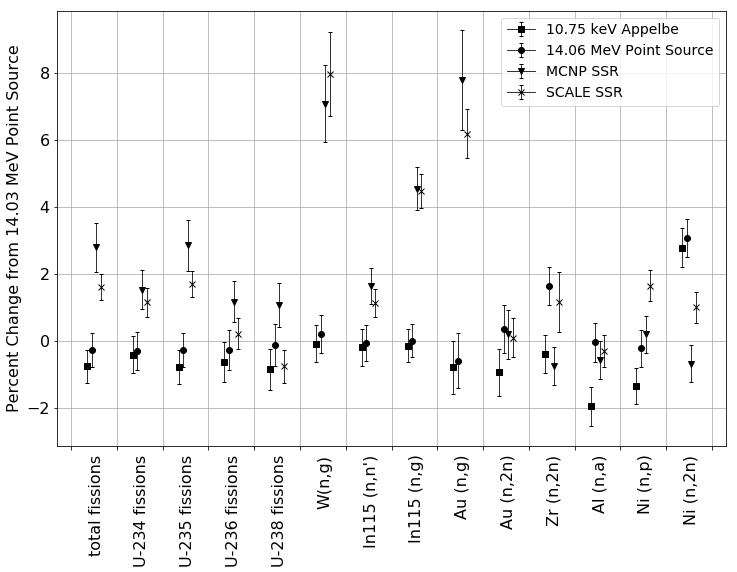
\includegraphics[width=\linewidth]{Figures/Chapter3/SourceComp.png}
	\caption[Comparison of results based on NIF source term. The statistical uncertainties of the underlying datasets are all less than 1\%]{Comparison of results based on NIF source term. The statistical uncertainties of the underlying datasets are all less than 1\%. Utilizing a higher energy source term provides larger production of threshold reactions while including the room return increases the thermal reactions.}
	\label{fig:srccomp}
\end{figure}

The comparison highlights a few key details that affect the solution set as a function of source neutron energy and the inclusion of the room return. 
First, source distributions containing higher energy neutrons (Appelbe or 14.06 MeV) affected the threshold reactions by as much as 2\%. 
This is due to the increasing cross-section for the threshold reactions at higher energy.  
Second, the thermal reactions increased substantially by including the room return and backscatter from the DIM. 
The down-scattered neutrons have lower energy and contributed more to the total response for the non-threshold reactions. 
%Last, the comparison between MCNP and SCALE SSR results was generally consistent. 
%The deviations from the mean were not systematically distributed as highlighted in Table \ref{table:act_sum}. 

\section{Statistical Analysis Tests}

The statistical tests utilized for this research included the Chi-squared statistic, the Pearson correlation coefficient, and the Kolmogorov-Smirnov (K-S) statistic. 
The Chi-squared is primarily utilized to test categorical distributions to assess if the results are governed by the expected distribution. % This is why it doesnt work for spectra! I can't find a source except for stack exchange, but all of the examples for calculating chi^2 online and in Taylor use it on discrete categories. 
The Pearson correlation coefficient and KS statistic both provide information regarding the similarity of two distributions. 

\noindent \textbf{1. Chi-squared Statistic}

\

\ The chi-squared statistic ($\chi^{2}$) is a useful tool for the interpretation of categorical results to expected values. 
The reduced $\chi^{2}$, as used in the foil activation neutron flux unfolding, is \cite{Taylor}
	
\begin{equation} \label{eq:chi}
\dfrac{\chi^2}{\nu}= \dfrac{1}{\nu}\sum_{i=1}^{n} \; (\dfrac{\textit{observed value - expected value}}{\textit{observed standard deviation }})^2.
\end{equation}

\ The degrees of freedom are the number of measurements in one data set minus one for the case of comparing two data sets of equal size. 
The degrees of freedom are defined with the observed data points and parameters computed to fit the equation. 

\ The ratio, $\chi^{2}/\nu$, can be used to assess goodness of fit between two distributions. 
The expected value for $\chi^{2}/\nu$ is unity if the calculated distribution is described by the expected distribution. 
A $\chi^{2}/\nu$ value much greater than one indicates that there is indeed a difference between the expected and observed distributions. 

\ The null hypothesis for the $\chi^{2}$ statistic is that the two sets of data are governed by the expected distribution. The test of independence shows the probability of rejecting this null hypothesis. 
The p-value can be used to compare the results of the expected distribution to the calculated $\chi^{2}/\nu$. 
The p-value is the probability of finding a larger $\chi^{2}/\nu$, given the calculated result. A small p-value ($<$0.05) signifies there is a strong significance level for the results not being governed by the expected distribution. P-values above the cutoff significance level fail to reject the null-hypothesis. A p-value of 0.05 or greater is generally accepted as statistically significant; however, this can change depending on the field of study.

\noindent \textbf{2. Pearson Correlation Coefficient}

\

\ The Pearson correlation coefficient provides a measure of the linear relationship between two sets of data. 
This metric is often used for comparative signal analysis. 
Like the $\chi^{2}$ statistic, the Pearson correlation coefficient is best suited for normally distributed data. 
Additionally, the statistic is meant for linear datasets, so a non-linear function correlation may be misrepresented. 
The formula for the Pearson correlation coefficient is given as a function of ``\textit{n}" data points for two distributions defined by points $x_{i}$ and $y_{i}$ as

\begin{equation} \label{eq:pearsonR}
r = \dfrac{n\sum{x_{i}y_{i}-(\sum{x_{i}}\sum{y_{i}})}}{ \sqrt{ n \sum{x_{i}^2}-(\sum{x_{i}})^2}\sqrt{n \sum{y_{i}^2}-(\sum{y_{i}})^2}}.
\end{equation}

\ The null hypothesis of this statistic is that there is no correlation between the two datasets. The p-value indicates the probability of an uncorrelated system producing a correlation coefficient at least as large in magnitude. Small p-values ($<$0.05) indicate a statistically significant Pearson correlation coefficient. 

\noindent \textbf{3. Kolmogorov-Smirnov (K-S) Statistic}

\

\ The K-S two-sample statistic compares the cumulative distribution functions (CDF) between two sets of data. 
The K-S statistic provides information on the relative magnitude of the distributions, so it is useful in combination with the Pearson correlation coefficient to quantify the similarity between two distributions.  
The K-S statistic is given as a function of the supremum (maximum) between the expected and observed CDF as shown in Equation \ref{eq:KS}.
The null hypothesis for this test is that the two samples were drawn from the same distribution. 
Unlike the other statistical tests shown earlier, a large p-value ($>$ 0.05) from the K-S statistic fails to reject the null hypothesis. 

\begin{equation} \label{eq:KS}
D  \ = \ \sup\limits_{x} \mid CDF_{exp}(x) - CDF_{obs}(x)\mid
\end{equation}
 



			
% Methodology
\chapter{Research Schedule}
\label{chap:ResearchSchedule}
\ The planned research schedule is heavily weighted on computational tasks. 
Bridgman will be the main high performance computer (HPC) utilized for analysis. 
Savio at UC-Berkley will be used to run Coeus for ETA-2 and ETA-SPNS. 
Due to the long nature of SAMPLER runs, the original ETA will be analyzed first on Bridgman. 
Figures \ref{fig:Cal1} to \ref{fig:Cal3} summarize a weekly schedule. 
The analysis periods are filled with many sub-tasks (plotting, $\chi^{2}$, running into errors, ect.)

\begin{figure}[ht]
	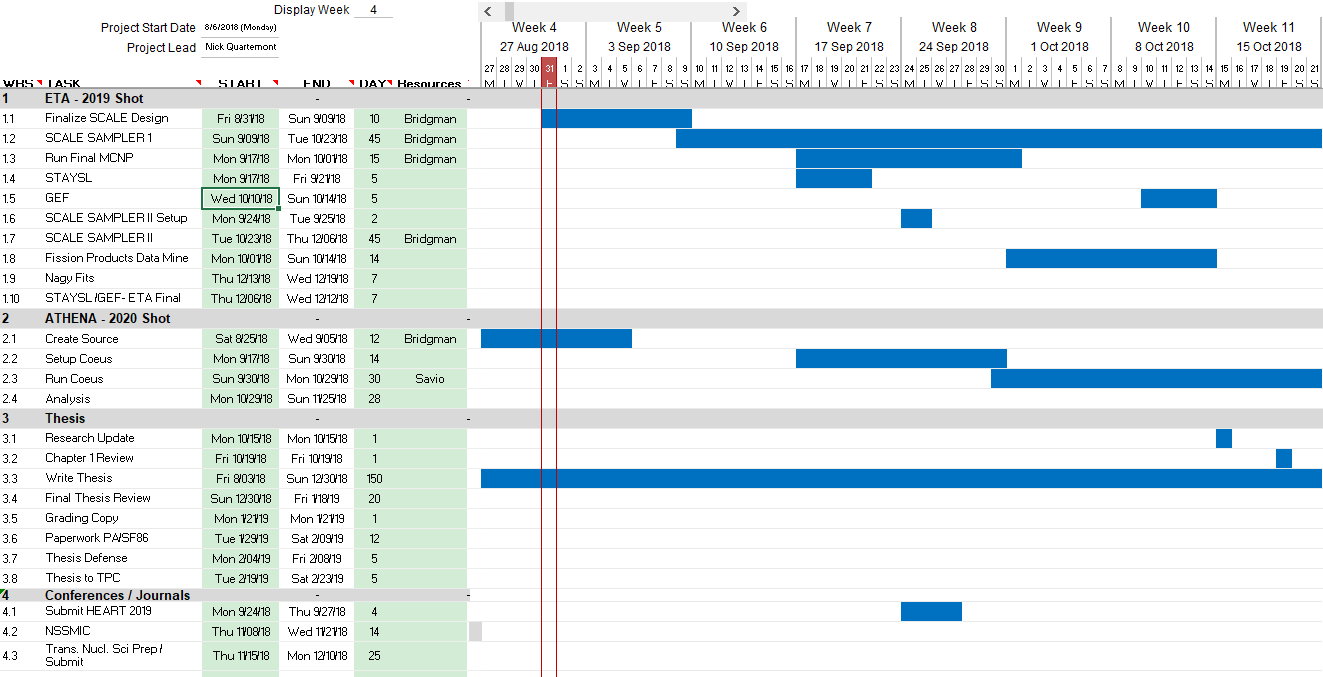
\includegraphics[width=\linewidth]{Figures/Chapter4/Cal1.png}
	\caption{Research schedule part 1}
	\label{fig:Cal1}
\end{figure} 

\begin{figure}[ht]
	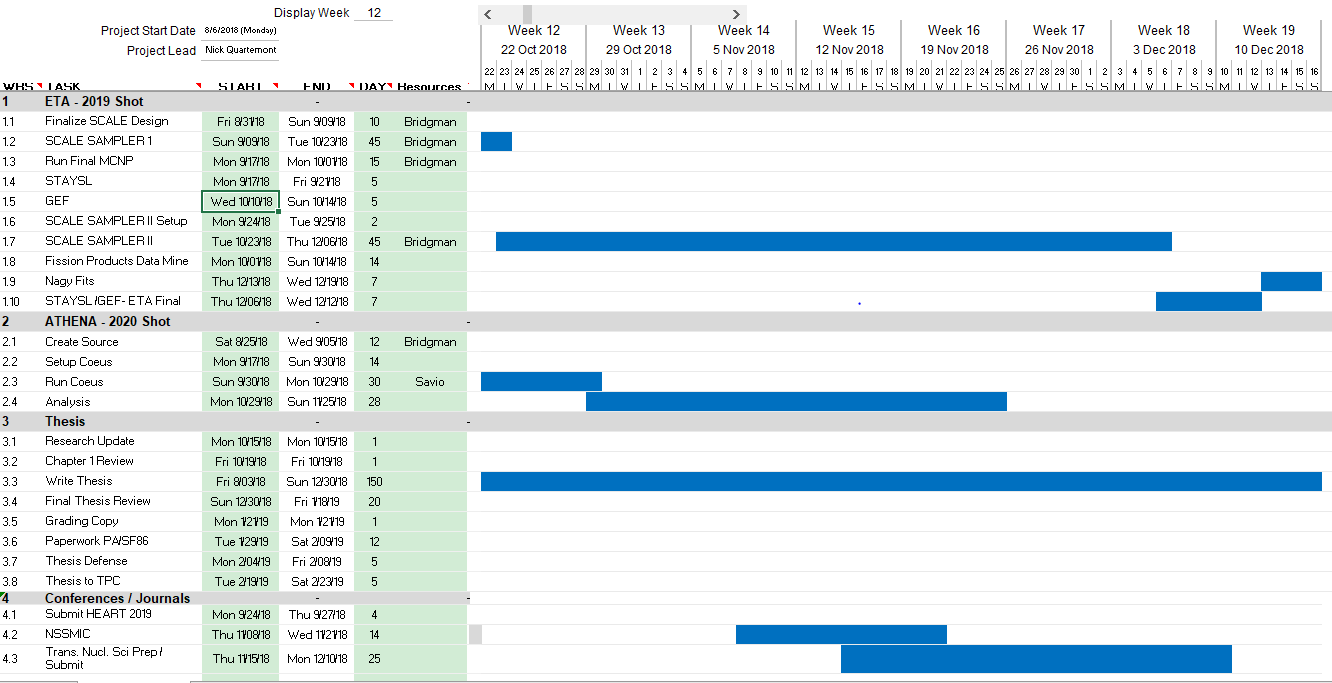
\includegraphics[width=\linewidth]{Figures/Chapter4/Cal2.png}
	\caption{Research schedule part 2}
	\label{fig:Cal2}
\end{figure} 
\begin{figure}[ht]
	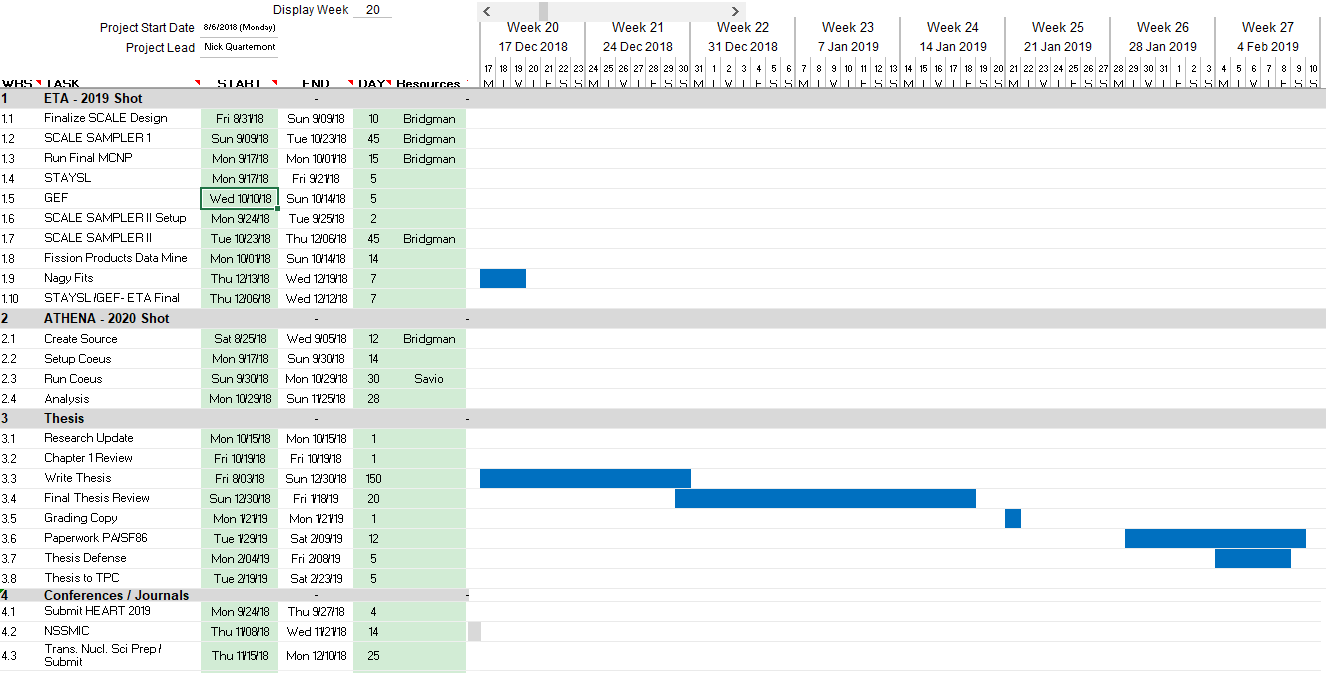
\includegraphics[width=\linewidth]{Figures/Chapter4/Cal3.png}
	\caption{Research schedule part 3}
	\label{fig:Cal3}
\end{figure} 

% Thesis
\chapter{Results}
\label{chap:Results}
\ This sections provides the simulated ETA results including the propagation of systematic nuclear data uncertainty. 
The neutron flux timing profile does not include the $\sigma_{sys}$ as the source mapping removed the time history data from the initial transport problem. 
First, the Monte Carlo simulation results pertaining to the neutron flux environment and foil pack activations are provided. 
The Monte Carlo results determined the effect of nuclear data covariance on the radiation transport simulation. 
Covariance analysis was only performed on ETA, not the objective TN+PFNS. 
As such, the final results are indicated by the MCNP-derived mean value with the bootstrapped uncertainty from the Sampler trials performed.
Next, the results of the neutron flux unfolding are shown which indicate the level of confidence of the foil pack to unfold the neutron flux for the ETA experiment. 
Finally, the fission product distribution and individual isotope production are provided. 

\section{ETA Monte Carlo Simulation Results}
\subsection{ETA Performance - Neutron Fluence Environment Comparison to TN+PFNS}

\ The main objective of ETA is to spectrally shape the DT source neutrons to the TN+PFNS.
Therefore, the spectrum achieved is a key metric for determining the performance of ETA.  
Figure \ref{fig:flux11} displays the nominal neutron fluence on the HEU foil as a function of energy with $\sigma_{stat}$ for the continuous energy neutron transport calculations.  
 
\begin{figure}[!htbp]
	\centering
	\vfill
	\subfigure[Logarithmic energy scale]{\includegraphics[width=13cm]{Figures/Chapter4/NeutronFlux/CE_Fluence_leth_c.png}}
	\vfill
	\subfigure[Linear energy scale]{\includegraphics[width=13cm]{Figures/Chapter4/NeutronFlux/CE_Fluence_leth_c_lin.png}}
	\vfill
	\caption{Neutron fluence per unit lethargy for SCALE MAVRIC, MCNP and objective TN+PFNS spectra. Only $\sigma_{stat}$ is captured for these results.}
	\label{fig:flux11}
\end{figure}

\ Overall, there is broad neutron spectral agreement between the TN+PFNS and ETA fluence. 	
Comparing the nominal values, there are a few main areas of disagreement between the ETA result and TN+PFNS. 
First, below 50 keV, there is an increase in thermal neutrons in the ETA simulations relative to the objective spectrum; however, this portion of the spectrum only represents $\sim$1\% of the ETA fluence. 
The NIF room return and low-A spectral shaping components contribute to the majority of this fluence.
Additionally, from 7 to 14 MeV there are relatively large differences caused by the method used to generate the TN+PFNS.
Godiva, composed solely of HEU, has very few pathways to populate this region. Inelastic scattering and (n,xn) reactions often completely skip over this energy range, and there would need to be many elastic scattering events to populate this energy range from the 14 MeV fusion source. 
The 14 MeV region disagreement is caused by the lack of attenuation of the source neutrons from weight constraints of the ETA design. 
Also above 14 MeV, there is a severely depressed neutron flux in ETA. 
A portion of the disagreement was caused by the mono-energetic source implementation instead of the ion temperature broadened distribution \cite{Appelbe2014}. 

A summary of the fractional fluence of the TN+PFNS and ETA is shown in Table \ref{table:frac_flux} which provides insight on the largest areas of disagreement between the ETA achieved neutron spectrum and the objective TN+PFNS. 
The deviations produced are theoretically discernible within the experimental foil activation portion of the experiment. 
However, the fission product distribution predicted from each energy dependent fluence is currently not as precise. 
The largest portion of the spectrum is the PFNS, and the ETA neutron fluence spectrum matches the fractional fluence over this energy range very well. 

\begin{table}[htb!]
	\centering
	\caption{Five-energy group fractional fluence for ETA design compared to TN+PFNS}
	\label{table:frac_flux}
	\setlength\extrarowheight{2.5pt}
\begin{tabular}{|c|c|c|c|}
	\hline
 & \multicolumn{2}{c|}{Fractional Fluence} & \multirow{2}{*}{\begin{tabular}[c]{@{}c@{}}ETA \% difference\\  from TN+PFNS\end{tabular}} \\ \cline{1-3}
Energy Range & ETA $\Phi$ & TN+PFNS $\Phi$ &  \\ \hline
	0 - 3.4 keV & 3.24E-04 & 7.23E-05 & 350 \\ \hline
	3.4 keV - 0.11 MeV & 4.85E-02 & 3.80E-02 & 28 \\ \hline
	0.11 MeV - 6.4 MeV & 7.83E-01 & 8.23E-01 & -5 \\ \hline
	6.4 - 10 MeV & 1.93E-02 & 1.31E-02 & 48 \\ \hline
	10 - 19.6 MeV & 1.49E-01 & 1.26E-01 & 19 \\ \hline
	\end{tabular}
\end{table}

\ Two statistical tests were conducted for additional confidence in the performance of ETA to spectrally shape the NIF source to the TN+PFNS. 
The results of the Pearson correlation coefficient and K-S statistic are summarized in Table \ref{table:flux_stats}. 
The $H_{0}$ results indicate that there was a strong correlation between the data sets and the samples were likely drawn from the same distribution.
The interpretation of the Pearson correlation coefficient result indicates that no correlation between the data sets can be rejected with strong significance, and the K-S statistic indicates the null hypothesis that the samples were drawn from the same distribution could not be rejected. 
The results indicate that the future experiment will succeed in achieving the TN+PFNS neutron environment based on the MCNP calculated neutron spectrum. 

\begin{table}[htb!]
	\centering
	\caption{Statistical test result comparisons between TN+PFNS and ETA performance.}
	\label{table:flux_stats}
	\setlength\extrarowheight{2.5pt}
	\begin{tabular}{|c|c|c|c|}
		\hline
& \begin{tabular}[c]{@{}c@{}}Pearson Correlation \\ Coefficient \\ (p-value)\end{tabular} & \begin{tabular}[c]{@{}c@{}}K-S Statistic \\ (p-value)\end{tabular} & $H_{0}$ \\ \hline
\begin{tabular}[c]{@{}c@{}}TN+PFNS \\ versus \\ MCNP SSR\end{tabular} & 0.90 (p $\ll$ 0.05) & 0.11 (p = 0.94) & \begin{tabular}[c]{@{}c@{}}Pearson - Rejected \\ K-S - Failed to Reject\end{tabular} \\ \hline
\begin{tabular}[c]{@{}c@{}}MCNP SSR \\ versus \\ SCALE MAVRIC \\ Mapped SSR\end{tabular} & 0.9999 (p $\ll$ 0.05) & 0.067 (p = 1.0) & \begin{tabular}[c]{@{}c@{}}Pearson - Rejected \\ K-S - Failed to Reject\end{tabular} \\ \hline
	\end{tabular}
\end{table}

\ The nominal MCNP simulated value was utilized to determine the similarities between the TN+PFNS and ETA; however, the affect of nuclear data covariance on the neutron transport operated to provide a variability in the expected differential neutron fluence. 
The neutron flux uncertainty mapped to the 46 group structure DPLUS in comparison with the TN+PFNS is shown in Figure \ref{fig:flux31}.
The systematic uncertainty was mapped as described in Section \ref{Mapping}. 
The fluence is shown per unit lethargy to remove binning artifacts.

\begin{figure}[!htbp]
	\centering
	\vfill
	\subfigure[Logarithmic energy scale]{\includegraphics[width=13cm]{Figures/Chapter4/NeutronFlux/Sys_Fluence_leth_c.png}}
	\vfill
	\subfigure[Linear energy scale]{\includegraphics[width=13cm]{Figures/Chapter4/NeutronFlux/Sys_Fluence_leth_c_lin.png}}
	\vfill
	\caption[Neutron fluence per unit lethargy scale for Sampler, MCNP and objective TN+PFNS spectra.]{Neutron fluence per unit lethargy scale for Sampler, MCNP and objective TN+PFNS spectra. The MCNP and objective TN+PFNS neutron spectrum are provided in the DPLUS group structure with  $\sigma_{stat}$ for these results. The Sampler results are presented in the collapsed 66 group structure with both $\sigma_{stat}$ and $\sigma_{sys}$ captured for this result.}
	\label{fig:flux31}
\end{figure}

\ The nominal value for each flux bin in Sampler is centered on the unperturbed nuclear data transport as expected because the cross-sections were sampled from a multivariate normal distribution.
Additionally, the fluence results highlight the issue of different bin structures and the requirement to estimate the uncertainty for alternative bin structures. 
The 252 group and continuous energy MCNP results have very similar characteristics; however, the 252 group bin structure is much coarser at high energy.  
The uncertainty results calculated approximately 4\% uncertainty for a large percentage of the spectrum and rising to near 100\% where $\sigma_{stat}$ was large. 
The form of the uncertainty is discussed further in Section \ref{UncertDiscuss}.
Although the DPLUS library was important for comparing to the objective spectrum, the main target group structure was the 129 group STAYSL format. 

\subsection{STAYSL Neutron Fluence with Mapped Systematic Uncertainty}\label{UncertDiscuss}

\ The 129 group STAYSL structure is used for the group structure for the neutron flux unfolding. 
This group structure has fine resolution at high energy which allowed for higher fidelity unfolding of the primarily high energy ETA spectrum. 
The uncertainty from the Sampler bin structure mapped to the 129 group format is shown in Figure \ref{fig:fluxu21}.

\begin{figure}[!htbp]
	\centering
	\vfill
	\subfigure[Logarithmic energy scale]{\includegraphics[width=12.5cm]{Figures/Chapter4/NeutronFlux/Uncertainty_c4.png}}
	\vfill
	\subfigure[Linear energy scale]{\includegraphics[width=12.5cm]{Figures/Chapter4/NeutronFlux/Uncertainty_c4_linlin.png}}
	\vfill
	\caption[Neutron fluence uncertainty from the Sampler 252-group structure mapped to the 129-group STAYSL structure.]{Neutron fluence uncertainty from Sampler 252-group structure mapped to the 129 group STAYSL structure. The total uncertainty for Sampler (solid black) and STAYSL (dash-dot blue) includes $\sigma_{sys}$ from the nuclear data covariance and $\sigma_{stat}$ from the Monte Carlo simulation.}
	\label{fig:fluxu21}
\end{figure}

\ The $\sigma_{sys}$ is mapped by midpoint energy bin linear interpolation.
This is a reasonable approximation method due to the behavior of the uncertainty as shown in Figure  \ref{fig:fluxu21}. 
Alternative mapping schemes may have been more appropriate if the uncertainty was not relatively constant. 
$\sigma_{sys}$ dominated over $\sigma_{stat}$ for nearly the entire neutron spectrum. 
At energies close to the source energy of 14 MeV, the total uncertainty is approximately 4-6\% which is near the uncertainty of the total scattering cross-section of tungsten and bismuth in this energy range. 
The intermediate energies between 0.01 and 8 MeV comprise a large portion of the neutron fluence and had total uncertainties of approximately 3-4\%. 
Due to multiple pathways to populate the peak of the PFNS, this region of the spectrum is affected less than others. 
The $\sigma_{stat}$ and $\sigma_{sys}$ are nearly the same magnitude at very high energy ($>$ 14 MeV) and low energy ($<$ 1 keV) where the neutron population is greatly reduced.
In these regions $\sigma_{stat}$ is a much more significant contribution to the overall uncertainty, which generally is approximately 10\%, but approached 100\% at the lowest energy bins. 

\ The ETA fluence in the 129-group STAYSL structure with mapped uncertainties is shown in Figure \ref{fig:fluxu41} in comparison with the SCALE/Sampler 252-group results from Figure \ref{fig:flux31}.
The STAYSL format again matched the characteristics of the 252 group format as seen with the DPLUS format; however, the bin width near the DT fusion source neutrons is smaller resulting in a more defined peak. 
Up-sampling in this region due to the finer resolution required the assumption that the uncertainty is relatively insensitive to group structure.  
Additionally, the nominal SCALE 252-group results were compared to the Sampler bootstrapped values, which showed that the mean Sampler value is centered on the nominal unperturbed nuclear data case. 

\begin{figure}[!htbp]
	\centering
	\vfill
	\subfigure[Logarithmic energy scale]{\includegraphics[width=13cm]{Figures/Chapter4/NeutronFlux/LethargyFlux_c_STAYSL.png}}
	\vfill
	\subfigure[Linear energy scale]{\includegraphics[width=13cm]{Figures/Chapter4/NeutronFlux/LethargyFlux_c_STAYSL_lin.png}}
	\vfill
	\caption{The 129 group STAYSL fluence compared to the Scale 252 group nominal fluence and Sampler values.}
	\label{fig:fluxu41}
\end{figure}


\subsection{Neutron Flux Timing Profile}

\ Two major characteristics of a neutron flux environment for use in certification testing are the total fluence of neutrons and the temporal domain. 
The incident fluence on the HEU foil for the modeled ETA experiment is 4.9 $\times$ 10$^{11}$ n cm$^{-2}$ $\pm$ 1.4\%. 
The time that the neutrons interacted with the volume has implications for applicability of the ETA concept to radiation effects testing. 
The neutron fluence per unit area from an unshaped point source with a strength of 3.7 $\times$ 10$^{15}$ neutrons at 29 centimeters (distance from the source to the ETA foils) is 3.5 $*$ 10$^{11}$ n cm$^{-2}$, so there the net neutron population with ETA is increased from the spherical divergence approximation.
The cumulative fluence on the HEU foil as a function of time is shown in Figure \ref{fig:timing1}. 

\begin{figure}[!htbp]
	\centering
	\includegraphics[width=13cm]{Figures/Chapter4/NeutronFlux/U_Fluence_timing.png}
	\caption{Cumulative neutron fluence on HEU foil as a function of time broken into four broad energy groups.}
	\label{fig:timing1}
\end{figure}

\ The total neutron pulse length in the ETA cavity is approximately 10 shakes or 100 nanoseconds. This was determined with a time binned tally in MCNP where the neutron fluence is grouped in time histories as well.  
The uncollided source neutrons arrive at the foil in approximately 0.6 shakes, consistent with the time required for a 14.03 MeV neutron to travel from the source to the HEU foil. 
The source neutrons make up a negligible portion of the total fluence seen by the foils as most are downscattered to produce the objective TN+PFNS. 
The higher energy neutrons from 2 to 14 MeV take the shortest time to arrive at the HEU foil as expected because these neutrons are moving faster and generally experience only a few interactions. 
The mid-range energy neutrons from 0.1 MeV to 2 MeV encompassed the bulk of the neutron fluence and take a slightly longer time or path to interact with the foils. 
Finally, the lower energy neutrons below 0.1 MeV take approximately 15 shakes to completely pass through the foils; however, this portion of the spectrum is a very small percentage of the total fluence. 
For certification testing purposes, a notional electronic component would see the complete neutron fluence in 100 nanoseconds. 

\subsection{Foil Activation}

\ The resultant activity in the foils is presented in Table \ref{table:actfoil2}. 
The individual reactions from Table \ref{table:act_sum} in Section \ref{Benchmark} are combined with the radioisotope decay constant based on the half-life. 
The initial activity post-irradiation is compared to the activity at 2 hours, the anticipated time that the foil pack could be removed from the NIF for analysis. 12 hours is also shown to provide insight on the time requirement for starting the activation foil spectroscopy. 
The foil activities, on the order of a kiloBecquerel [kBq] with the exception of the indium foil, are acceptable for gamma-ray spectroscopy using the LLNL facilities. 
The indium product half-lives are relatively short in comparison to the other isotopes, so a higher activity allows for detection hours later. 

\begin{table}[htb!]
	\centering
	\caption{Foil activities predicted with bootstrapped nuclear data covariance uncertainty.}
	\label{table:actfoil2}
	\setlength\extrarowheight{2.5pt}
\begin{tabular}{|c|c|c|c|c|c|}
	\hline
\textbf{Product} & \textbf{$\mathbf{t_{1/2}}$} & \textbf{\begin{tabular}[c]{@{}c@{}}Initial\\ Activity \\ {[}kBq{]}\end{tabular}} & \textbf{\begin{tabular}[c]{@{}c@{}}$\mathbf{\Delta t = 2 hr}$ \\ Activity \\ {[}kBq{]}\end{tabular}} & \textbf{\begin{tabular}[c]{@{}c@{}}$\mathbf{\Delta t = 12 hr}$ \\ Activity\\ {[}kBq{]}\end{tabular}} & \textbf{\begin{tabular}[c]{@{}c@{}}Relative \\ Error \\ {[}\%{]}\end{tabular}} \\ \hline
	$\mathrm{^{89}Zr}$ & 78.41 hrs & 4.63 & 4.55 & 4.17 & 4.7 \\ \hline
	$\mathrm{^{57}Ni}$ & 35.6 hrs & 1.01 & 0.97 & 0.80 & 4.8 \\ \hline
	$\mathrm{^{58}Co}$ & 70.86 days & 0.74 & 0.74 & 0.74 & 2.5 \\ \hline
	$\mathrm{^{196}Au}$ & 6.17 days & 3.78 & 3.75 & 3.58 & 4.8 \\ \hline
	$\mathrm{^{198}Au}$ & 2.69 days & 2.98 & 2.92 & 2.62 & 2.6 \\ \hline
	$\mathrm{^{115}In^{m1}}$ & 4.49 hrs & 164 & 120 & 25.7 & 2.3 \\ \hline
	$\mathrm{^{116}In^{m1}}$ & 54.29 min & 1094 & 236 & 0.11 & 3.4 \\ \hline
	$\mathrm{^{24}Na}$ & 15 hrs & 13.8 & 12.6 & 7.93 & 4.6 \\ \hline
	$\mathrm{^{187}W}$ & 24 hrs & 5.79 & 5.46 & 4.09 & 4.1 \\ \hline
	$\mathrm{^{56}Mn}$ & 2.58 hrs & 23.5 & 13.7 & 0.93 & 20.0 \\ \hline
	\end{tabular}
\end{table} 

\ The bootstrapped uncertainty results show a fairly large variance in the foil activities produced. 
Uncertainty in the radioactive half-life is not propagated as it is comparatively negligible. 
The initial activity of most foils have an uncertainty of a few percent, but there is high uncertainty (20\%) in the $\mathrm{^{55}}$Mn reaction due to relatively large cross-section uncertainty over the activation range. 
Additionally, this reaction experiences more reactions with lower energy neutrons where the net transport uncertainty is greater. 
A histogram of the number of $\mathrm{^{58}}$Ni (n,2n), $\mathrm{^{27}}$Al (n,a), $\mathrm{^{115}}$In (n,g), and  $\mathrm{^{55}}$Mn (n,g) reactions compiled from the post-processed Sampler results is shown in Figure \ref{fig:act_histo}. 
The remaining histograms deviate minimally from these.
The results indicate a quasi-Normal distribution centered on the mean value determined from the non-perturbed nuclear data. 

\begin{figure}[!htb]
	\centering
	\includegraphics[width=15cm]{Figures/Chapter4/NeutronFlux/Foil_Histo.png}
	\caption{Histograms of several activation foil reactions produced with Sampler results.}
	\label{fig:act_histo}
\end{figure}


\ The contribution to the total uncertainty from neutron transport, as manifested in the fluence uncertainty, and reaction cross-section uncertainty is determined for the reactions that utilized the IRDFF nuclear data. 
Reactions that were completed solely in Sampler have this information convolved in the results and are not included in Table \ref{table:contributions}. 

\begin{table}[htb!]
	\centering
	\caption{Contributions to total uncertainty for activation reactions utilizing IRDFF nuclear data.}
	\label{table:contributions}
	\setlength\extrarowheight{2.5pt}
	\begin{tabular}{|c|c|c|c|}
		\hline
		\textbf{Reaction} & \textbf{$\sigma_{total}$ {[}\%{]}} &\textbf{ Transport $\sigma$ {[}\%{]}} & \textbf{Reaction $\sigma$ {[}\%{]}} \\ \hline
		$\mathrm{^{90}Zr}$ (n,2n) $\mathrm{^{89}Zr}$ & 4.66 & 4.60 & 0.78 \\ \hline
		$\mathrm{^{58}Ni}$ (n,2n) $\mathrm{^{57}Ni}$ & 4.76 & 4.57 & 1.34 \\ \hline
		$\mathrm{^{58}Ni}$ (n,p) $\mathrm{^{58}Co}$ & 2.50 & 2.14 & 1.29 \\ \hline
		$\mathrm{^{197}Au}$ (n,2n) $\mathrm{^{196}Au}$ & 4.84 & 4.63 & 1.42 \\ \hline
		$\mathrm{^{115}In}$ (n,n') $\mathrm{^{115}In^{m1}}$ & 2.33 & 1.85 & 1.42 \\ \hline
		$\mathrm{^{115}In}$ (n,g) $\mathrm{^{116}In^{m1}}$ & 3.45 & 2.59 & 2.28 \\ \hline
		$\mathrm{^{27}Al}$ (n,a) $\mathrm{^{24}Na}$ & 4.62 & 4.59 & 0.45 \\ \hline
	\end{tabular}
\end{table}

\ The uncertainties with only the transport uncertainty included are determined by running the post-processing script with and without sampling the reaction cross-sections. The baseline case without sampling the reaction cross-section reflects the uncertainty due to solely transport related uncertainties. Likewise, the transport uncertainty convolved with the reaction uncertainty are determined by including the reaction pertubation. 
The reaction uncertainty was determined by assuming the transport uncertainty and reaction uncertainty were added in quadrature based on the relative errors ($R\: \propto \sigma\phi \rightarrow  (\sigma_{R}/R)^{2} = (\sigma_{\phi}/\phi)^{2} + (\sigma_{\sigma}/\sigma)^{2}$). 

The uncertainty contributions are largely dominated by the fluence uncertainty as expected since the reactions were chosen for low uncertainty over the activation range. 
The fluence uncertainty is nearly constant for all high energy threshold reactions covering the TN portion of the spectrum, which is caused by all four reactions having a very similar functional form and energy coverage. 
In general, non-threshold reactions experienced lower transport uncertainty because the reaction occurred over all energy ranges which reduces volatility in the integral reaction mechanism. 	
	
\section{STAYSL Neutron Flux Unfolding Results}

\ The 129-group STAYSL unfolded spectrum is shown in Figure \ref{fig:unfold1}.
The results utilize the starting guess MCNP spectrum outlined in Figure \ref{fig:fluxu41}.
The guess spectrum uncertainty provide a physics-based constraint to the range of spectrum adjustments performed by STAYSL. 

\ STAYSL was executed on all 182 sets of foil activities from Sampler to build a distribution of possible modeled experimental outcomes. 
The largest $\chi^{2}$ trial and bootstrapped neutron fluence from all trials were added to Figure \ref{fig:unfold1} for comparison with the initial guess MCNP spectrum.
Additionally, the 5-95\% activation ranges for each reaction are shown indicating the region  informed in the unfolding procedure by a given reaction.  


\begin{figure}[!htbp]
	\centering
	\vfill
	\subfigure[Logarithmic energy scale]{\includegraphics[width=13cm]{Figures/Chapter4/Unfold/STAYSL_unfold.png}}
	
	\subfigure[Linear energy scale]{\includegraphics[width=13cm]{Figures/Chapter4/Unfold/STAYSL_unfold_lin.png}}
	\vfill
	\caption[STAYSL unfolded spectra per unit lethargy for nominal guess, largest deviation, and bootstrapped values.]{STAYSL unfolded spectra per unit lethargy for nominal guess, largest deviation, and bootstrapped values. The 90\% activation range represents the saturation region for the foil reactions utilized in the neutron flux unfolding.}
	\label{fig:unfold1}
\end{figure}

\ An important result from the unfolding procedure is defining the region that produced 90\% of the activation for each reaction. 
These regions are important for determining the coverage of the activation foil set. 
Overall, the threshold reactions provide coverage at high energy and were mostly saturated by the 14 MeV peak. 
However, lower energy threshold reactions provide coverage between approximately 1 and 14 MeV. 
Finally, the thermal reactions are functionally epithermal neutron foils based on the reactions with the ETA neutron spectrum. 
Although these thermal reactions are not best suited for the epithermal region where the cross-section is low, they prove beneficial by having a low cross-section at high energy where the vast majority of neutrons are. 
This low cross-section allows for higher resolution in unfolding the epithermal portion of the neutron spectrum at the expense of having relatively little coverage at thermal energies. 

\ Additionally, the residual fluence between the MCNP guess spectrum and STAYSL calculated neutron fluence provides information on where the guess spectrum deviates from the calculated activities. The relative residual fluence between the MCNP guess neutron spectrum and the STAYSL calculated neutron spectrum with unperturbed foil activities is shown in Figure \ref{fig:unfold50}. 

\begin{figure}[!htbp]
	\centering
	\vfill
	\subfigure[Logarithmic energy scale]{\includegraphics[width=13cm]{Figures/Chapter4/Unfold/STAYSL_MCNP_Residuals_Rel_log.png}}
	\vfill
	\subfigure[Linear energy scale]{\includegraphics[width=13cm]{Figures/Chapter4/Unfold/STAYSL_MCNP_Residuals_Rel.png}}
	\vfill
	\caption{Relative residual neutron fluence between the MCNP guess spectrum and the STASYL unfold with unperturbed foil activities in 129 group STAYSL structure.}
	\label{fig:unfold50}
\end{figure}

\ The relative residual fluence between the guess spectrum and the changes calculated with STAYSL also highlight the areas that adjustments are made. 
The neutron fluence was reduced at low energy; however, this can be attributed to the large uncertainty. The remainder of the neutron fluence was slightly increased aside from the largest energy bin, which indicates that the apparent isotope activity is slightly larger than calculated. The increase to the bulk of the neutron fluence is indicative of slight changes to the neutron spectrum in the sample cavity. Furthermore, the changes made to the entire spectrum are well within uncertainty bounds. 

\ The $\chi^{2}$ results indicate that $H_{0}$, that the two sets of data were governed from the expected distribution, could not be rejected for most of the trials with high confidence. 
The $\chi^2$ is derived from the unfolded activities, not the neutron flux as the flux is not a categorical variable. 
The p-value reflects the probability of finding a greater $\chi^{2}$. 
The $\chi^2$ for the nominal guess, largest sample, and bootstrapped unfolded activities are 0.36, 8.3, and 1.3 with p-values of 0.96, $\ll$ 0.05, and 0.22, respectively. 
The p-values indicate the probability of achieving a larger $\chi^2$ given the results, so the nominal case is within reasonable expectation while the largest $\chi^2$ value is rejected with strong significance. 
The bootstrapped activity p-value is closer to the rejection value of 0.05, but the p-value is large enough to not reject the unfolded activities.  
It is important to note that the $\chi^2$ values did not include the fluence uncertainty, only the bootstrapped activity uncertainty as outlined in Section \ref{STAYSLthing}.
The distribution of $\chi^2/\nu$ values for the set of trials is shown in Figure \ref{fig:chi2sfromunfold}. 

\begin{figure}[!htbp]
	\centering
	\includegraphics[width=13cm]{Figures/Chapter4/Unfold/Chi2_Histogram.png}
	\caption{Histogram of STAYSL unfolded ETA spectrum $\mathbf{\chi^2}$ for each unfolded trial.}
	\label{fig:chi2sfromunfold}
\end{figure}

\ The distribution of $\chi^2$ values peaks near 1; however, a non-negligible portion of the unfolding calculations provide results that rejected $H_{0}$. 
A few cross-sections may generally increase and other decrease which had a negative effect on the ability to unfold the spectrum. 
Of the 182 trials, the hypothesis that activities come from the expected distribution is not rejected 81.9\% of the time and rejected 18.1\% with 95\% confidence.

The distribution of the unfolded STASYL results compared to the TN+PFNS is shown in Figure \ref{fig:unfold10}. The TN+PFNS is binned into the 129 group STAYSL structure to allow for a direct comparison of the STAYSL results to the objective neutron spectrum. 
The TN+PFNS binned in the DPLUS format is very similar except at high energy, where there is more resolution to define the TN portion of the spectrum. 

\begin{figure}[!htbp]
	\centering
	\vfill
	\subfigure[Logarithmic energy scale]{\includegraphics[width=13cm]{Figures/Chapter4/Unfold/STAYSL_Fluence_log.png}}
	\vfill
	\subfigure[Linear energy scale]{\includegraphics[width=13cm]{Figures/Chapter4/Unfold/STAYSL_Fluence_lin.png}}
	\vfill
	\caption{STAYSL 129-group guess spectrum per unit lethargy compared to TN+PFNS in 129-group STAYSL structure.}
	\label{fig:unfold10}
\end{figure}

\ Each of the STAYSL unfolded neutron spectrum are compared to the TN+PFNS through the K-S statistic and the Pearson correlation coefficient . 
The value of the K-S statistic was 0.094 with a p-value of 0.61. 
The K-S statistic is statistically equivalent for each trial unfold because the TN portion dominated the difference between the STAYSL unfold and TN+PFNS. 
The 129 group format K-S statistic indicates again that the samples were drawn from the same distribution could not be rejected. 

\ The distribution of Pearson correlation coefficients and p-values are shown in Figure \ref{fig:unfold20}. 
The minimum Pearson correlation coefficient is approximately 0.82, corresponding to a p-value of near zero. This also serves as a compliment and verification for the 82\% not rejected foil activity $\chi^2$ results.
The largest coefficient is below 0.85 which has a p-value also near zero. 

\ The Pearson correlation coefficient performs worse with the 129 group STAYSL structure as an artifact of utilizing the modeled mono-energetic 14.03 source neutrons. 
The interpretation of each Pearson correlation coefficient result indicates again that no correlation between the data sets was rejected with strong significance, 
The Pearson correlation coefficient p-value from the 129 group structure is $\ll$ 0.05 and still well below a rejection region below 0.05, so the results further indicate spectral agreement between the ETA produced neutron flux in the sample cavity and the TN+PFNS.

\begin{figure}[!htbp]
	\centering
	\vfill
	\subfigure[Distribution of Pearson Correlation Coefficients]{\includegraphics[width=13cm]{Figures/Chapter4/Unfold/Pearson.png}}
	\vfill
	\subfigure[Distribution of p-values]{\includegraphics[width=13cm]{Figures/Chapter4/Unfold/Pearson_P.png}}
	\vfill
	\caption{STAYSL unfolded Pearson correlation coefficient distribution for independent samples.}
	\label{fig:unfold20}
\end{figure}

\section{Fission Products}

\ The fission product distribution and isotopes are the predicted observable quantity reflective of the neutron fluence incident on the HEU sample. 
First, the fissioning neutron energy spectra are described for $\mathrm{^{235}}$U and $\mathrm{^{238}}$U.
These spectra are used with the GEF and Nagy approaches to provide an estimate of the fission products expected to be produced in the HEU. 

\subsection{HEU Fission Spectra}

\ The energy-dependent neutron fluence convolved with the fission cross-section can be used to determine the fission rate as a function of energy for the various isotopes in the HEU foil.
The resultant HEU fissions as a function of energy for $\mathrm{^{235}}$U and $\mathrm{^{238}}$U are shown in Figure \ref{fig:flux51}.  

\begin{figure}[!htbp]
	\centering
	\vfill
	\subfigure[Logarithmic energy scale]{\includegraphics[width=13cm]{Figures/Chapter4/NeutronFlux/E_Fissions.png}}
	\vfill
	\subfigure[Linear energy scale]{\includegraphics[width=13cm]{Figures/Chapter4/NeutronFlux/E_Fissions_lin.png}}
	\vfill
	\caption{ETA HEU sample fissions in 46 group DPLUS group structure with $\sigma_{sys}$ included in the results.}
	\label{fig:flux51}
\end{figure}

\ The $\mathrm{^{235}}$U fissions provide a similar functional form to the ETA sample cavity fluence. 
However, lower energy fissions comprise a much larger relative contribution to the total fissions, which motivated the necessity for lower statistical uncertainty at lower energies. 
Still, the majority of the fissions were produced by neutrons above 0.1 MeV in $\mathrm{^{235}}$U. 
The isotope $\mathrm{^{238}}$U is a fissionable isotope with a threshold of approximately 1 MeV and is at a lower number density in the modeled HEU foil, so there are significantly fewer fissions overall. 
The remaining uranium isotopes are neglected as their contribution is negligible. 
The fission spectra here are utilized to provide the compound nucleus energy states for GEF. 

\subsection{GEF}

\ A comparison between the ETA produced fission products as calculated in GEF and the previously shown ENDF-published data is shown in Figure \ref{fig:fp1}. 
The resultant ETA fission product distribution is on average between the fast and high energy ENDF data. 
The error associated with the GEF results is largely due to the Monte Carlo approach utilized by GEF which included perturbations to the constants utilized in addition to the neutron flux uncertainty. 

\begin{figure}[!htbp]
	\centering
	\includegraphics[width=13cm]{Figures/Chapter4/FPs/GEF_ENDF.png}
	\caption{ETA fission product mass chain distribution calculated with GEF in comparison to ENDF values.}
	\label{fig:fp1}
\end{figure}

\ The resultant GEF mass chain distribution for ETA and the original objective TN+PFNS are displayed in Figure \ref{fig:fp2}. 
Overall, there is large agreement in reproducing the fission product distribution expected from the TN+PFNS.
The high uncertainty reflects the limited capability to predict mass chain fission products \textit{a priori}. 

\begin{figure}[!htbp]
	\centering
	\includegraphics[width=13cm]{Figures/Chapter4/FPs/ETA_vs_TNPFNS_FPs.png}
	\caption{TN+PFNS versus ETA fission product mass chain distributions calculated with GEF values.}
	\label{fig:fp2}
\end{figure}

\ The mass chain residual yields comparing ETA to the objective spectrum are shown in Figure \ref{fig:fp3}. 
There are a few areas of disagreement between the mean value of ETA and the TN+PFNS. 
The symmetric valley fission products are systematically larger due to the increased high energy flux produced by ETA as highlighted in Table \ref{table:frac_flux}. 
Accordingly, the is an increase in yield for asymmetric fission products mass chains.
However, neither are substantial compared to the error. 

\begin{figure}[!htbp]
	\centering
	\includegraphics[width=13cm]{Figures/Chapter4/FPs/Residuals_Obj_minus_ETA.png}
	\caption{Residual mass chain yields of ETA compared to TN+PFNS from GEF values.}
	\label{fig:fp3}
\end{figure}

\subsection{Nagy Fits}

\ The experimental data as a function of incident neutron energy is applied to the ETA fluence with Nagy fits. 
The Nagy fit values represent the cumulative fission product yield for the individual isotope. 
The experimental parameters for the exponential slope of the fit and yield at thermal fission are shown in Figures \ref{fig:nagy1} and \ref{fig:nagy2}. 

\begin{figure}[!htbp]
	\centering
	\includegraphics[width=13cm]{Figures/Chapter4/FPs/U_Fis_FitParam.png}
	\caption{Nagy fit experimental data exponential slope values as a function of selected isotopes atomic mass.}
	\label{fig:nagy1}
\end{figure}

\begin{figure}[!htbp]
	\centering
	\includegraphics[width=13cm]{Figures/Chapter4/FPs/U_Fis_FitParam_Y0_lin.png}
	\caption{Nagy fit experimental data thermal fission yields as a function of selected isotopes atomic mass.}
	\label{fig:nagy2}
\end{figure}

The results of the fitting parameters are consistent with expectations. 
The yield at thermal fission fitting value is very similar to the mass chain distributions outlined in Figure \ref{fig:U235Cumulative}. 
The exponential slope of the cumulative yield as a function of energy is small for wing and peak mass chains which generally decrease with increasing incident neutron energy. 
The cumulative yields above mass chain 145 also slightly increase with neutron energy. 
The symmetric valley fission product yield increases much more substantially as shown by the large values of the exponential slope near the 110 mass number. 

The resultant fission product yields are compared between ETA and the objective TN+PFNS in Table \ref{table:fps3} along with the relative activities compared to $\mathrm{^{95}}$Zr. 
The isotope $\mathrm{^{95}}$Zr has a longer half-life and a strong gamma-ray to use as a baseline for comparison to the other fission products. 

\begin{table}[htb!]
	\centering
	\caption[ETA and TN+PFNS produced Nagy fit cumulative fission product yield from experimental data.]{ETA and TN+PFNS produced Nagy fit cumulative fission product yield from experimental data. The fission product activities are compared to the longer-lived $\mathbf{^{95}}$Zr}.
	\label{table:fps3}
	
	\setlength\extrarowheight{2.5pt}
	\resizebox{\textwidth}{!}{%
		\begin{tabular}{|c|c|c|c|c|}
\hline
\multirow{2}{*}{\begin{tabular}[c]{@{}c@{}}\textbf{Fission} \\ \textbf{Product} \end{tabular}} & \multicolumn{2}{c|}{\textbf{Fission Product Yield {[}\%{]}}} & \multicolumn{2}{c|}{\textbf{Relative Activity to $\mathrm{^{95}Zr}$}} \\ \cline{2-5} 
& \textbf{ETA} & \textbf{TN+PFNS} & \textbf{ETA} & \textbf{TN+PFNS} \\ \hline
$\mathrm{^{91}Sr}$ & 5.34 $\pm$ 0.15 & 5.37 $\pm$ 0.08 & 141 $\pm$ 3.7\% & 141 $\pm$ 1.7\% \\ \hline
$\mathrm{^{92}Sr}$ & 5.38 $\pm$ 0.16 & 5.41 $\pm$ 0.10 & 516 $\pm$ 4.0\% & 517 $\pm$ 2.1\% \\ \hline
$\mathrm{^{95}Zr}$ & 6.03 $\pm$ 0.15 & 6.05 $\pm$ 0.06 & 1 $\pm$ 3.6\% & 1 $\pm$ 1.3\% \\ \hline
$\mathrm{^{97}Zr}$ & 5.71 $\pm$ 0.16 & 5.74 $\pm$ 0.08 & 87.0 $\pm$ 3.7\% & 87.0 $\pm$ 1.7\% \\ \hline
$\mathrm{^{99}Mo}$ & 5.62 $\pm$ 0.16 & 5.65 $\pm$ 0.08 & 21.7 $\pm$ 3.8\% & 21.7 $\pm$ 1.7\% \\ \hline
$\mathrm{^{103}Ru}$ & 3.20 $\pm$ 0.09 & 3.21 $\pm$ 0.05 & 0.867 $\pm$ 3.8\% & 0.864 $\pm$ 1.8\% \\ \hline
$\mathrm{^{105}Ru}$ & 1.41 $\pm$ 0.05 & 1.39 $\pm$ 0.04 & 81.3 $\pm$ 4.6\% & 79.7 $\pm$ 3.0\% \\ \hline
$\mathrm{^{109}Pd}$ & 0.32 $\pm$ 0.02 & 0.29 $\pm$ 0.02 & 6.01 $\pm$ 6.3\% & 5.31 $\pm$ 5.6\% \\  \hline
$\mathrm{^{111}Ag}$ & 0.28 $\pm$ 0.01 & 0.25 $\pm$ 0.01 & 0.399 $\pm$ 4.8\% & 0.350 $\pm$ 3.7\% \\ \hline
$\mathrm{^{112}Pd}$ & 0.27 $\pm$ 0.01 & 0.23 $\pm$ 0.01 & 3.22 $\pm$ 5.9\% & 2.82 $\pm$ 5.4\% \\ \hline
$\mathrm{^{113}Ag}$ & 0.20 $\pm$ 0.01 & 0.18 $\pm$ 0.01 & 9.50 $\pm$ 7.0\% & 8.30 $\pm$ 6.5\% \\ \hline
$\mathrm{^{115g}Cd}$ & 0.28 $\pm$ 0.01 & 0.25 $\pm$ 0.01 & 1.36 $\pm$ 5.6\% & 1.18 $\pm$ 4.9\% \\ \hline
$\mathrm{^{132}Te}$ & 4.32 $\pm$ 0.13 & 4.33 $\pm$ 0.07 & 14.3 $\pm$ 3.9\% & 14.3 $\pm$ 1.9\% \\ \hline
$\mathrm{^{140}Ba}$ & 5.56 $\pm$ 0.15 & 5.60 $\pm$ 0.07 & 4.63 $\pm$ 3.7\% & 4.65 $\pm$ 1.6\% \\ \hline
$\mathrm{^{141}Ce}$ & 5.46 $\pm$ 0.17 & 5.49 $\pm$ 0.10 & 1.78 $\pm$ 4.0\% & 1.79 $\pm$ 2.1\% \\ \hline
$\mathrm{^{143}Ce}$ & 5.06 $\pm$ 0.15 & 5.11 $\pm$ 0.09 & 39.1 $\pm$ 3.9\% & 39.3 $\pm$ 1.9\% \\  \hline
$\mathrm{^{144}Ce}$ & 4.69 $\pm$ 0.16 & 4.75 $\pm$ 0.11 & 0.175 $\pm$ 4.2\% & 0.176 $\pm$ 2.5\% \\ \hline
$\mathrm{^{147}Nd}$ & 2.08 $\pm$ 0.06 & 2.10 $\pm$ 0.03 & 2.01 $\pm$ 3.8\% & 2.02 $\pm$ 1.7\% \\ \hline
$\mathrm{^{149}Pm}$ & 1.01 $\pm$ 0.04 & 1.01 $\pm$ 0.03 & 4.83 $\pm$ 4.9\% & 4.84 $\pm$ 3.3\% \\ \hline
$\mathrm{^{151}Pm}$ & 0.47 $\pm$ 0.02 & 0.46 $\pm$ 0.02 & 1361 $\pm$ 5.5\% & 1341 $\pm$ 4.3\% \\ \hline
$\mathrm{^{153}Sm}$ & 0.18 $\pm$ 0.01 & 0.18 $\pm$ 0.01 & 0.982 $\pm$ 6.6\% & 0.969 $\pm$ 5.5\% \\ \hline
$\mathrm{^{156}Eu}$ & 0.028 $\pm$ 0.001 & 0.027 $\pm$ 0.001 & 0.020 $\pm$ 5.4\% & 0.019 $\pm$ 4.3\% \\ \hline
$\mathrm{^{161}Tb}$ & 0.0013 $\pm$ 0.00006 & 0.0011 $\pm$ 0.00004 & 0.0020 $\pm$ 5.5\% & 0.0017 $\pm$ 4.2\% \\ \hline
		\end{tabular}%
	}
\end{table}

\ The cumulative fission product yields in Table \ref{table:fps3} are mostly the precursor to the stable state. 
In the case where there are additional steps in the decay chain before the stable state, the independent yield of daughter isotopes often have negligible yields.
Therefore, all of the decay feeding passes through these cumulative fission product isotopes with the exception of $\mathrm{^{132}}$Te. 
$\mathrm{^{132}}$Te is in competition with the daughter isotope $\mathrm{^{132}}$I. 
Therefore, the experimental yields, with the exception provided, enable lower uncertainty approximations of the mass chain yields than GEF where experimental data exists. 
Figure \ref{fig:fp4} displays the ETA results with Nagy fit data in their given mass chains, which substantially improves the picture of predicting fission product yields. 
In particular, these isotopes serve as excellent verification data points for the ETA experiment in confirming the ETA fission products. 

\begin{figure}[!htbp]
	\centering
	\vfill
	\subfigure[Logarithmic energy scale]{\includegraphics[width=13cm]{Chapter4/FPs/GEF_ENDF_Nagy.png}}
	\vfill
	\subfigure[Linear energy scale]{\includegraphics[width=13cm]{Chapter4/FPs/GEF_ENDF_Nagy_lin.png}}
	\vfill
	\caption{Experimental predictions of ETA mass chain yields utilizing GEF and Nagy fit data where selected experimental measurements exist in literature.}
	\label{fig:fp4}
\end{figure}

In a real world scenario, these fallout particles may be collected on the ground or air as with the CTBT monitoring. 
The Department of Defense Fallout Prediction System, DELFIC, can model the fallout distribution on the ground following a nuclear event with the Fallout Planning Tool user interface \cite{DELFIC, Jodoin2011}. 
A 10 KT fission weapon at ground level was modeled using weather data from 16 August 2017 at Wright-Patterson Air Force Base, OH. 
The ground dispersal in effective fissions per meter square from the 140 mass chain is shown in Figure \ref{fig:delfic}.
The 140 mass chain was chosen because the yield does not change drastically with the fissioning system. 
The modeled ETA results produced an equivalent number of fissions as in 0.1 m$^{2}$ of the lowest contour band. 
As the number of fissions are increased, the quality of the sample is more useful. 
Nevertheless, the modeled ETA performance has promising capabilities to create spectrally accurate fission product debris. 

\begin{figure}[!htbp]
	\centering
	\includegraphics[width=13cm]{Figures/Chapter5/FP_m2.png}
	\caption{DELFIC calculated fission product equivalent fissions on the ground per unit area from mass chain 140.}
	\label{fig:delfic}
\end{figure}

	
% Results	

\backmatter
\singlespace
%\bibliographystyle{Back/thesnumb3}
%\bibliographystyle{Back/agu}
\bibliographystyle{Back/IEEEtran} 						
\bibliography{Back/MyBibliography}
%\bibliographystyle{unsrt}
  \addtocontents{toc}{\vspace{10pt}} %space between bibliography and vita in toc
\clearpage

%
%% !TEX root = ../SteadmanThesis.tex

%\addcontentsline{toc}{chapter}{Vita}
%\begin{center}
%\textbf{Vita}
%\end{center}
%\vspace{.35in}

 \addcontentsline{toc}{chapter}{Vita}
    \begin{center}
	\bfseries Vita
    \end{center}
    \vspace{2em}

\doublespace
Captain Lindon Steadman was born in Murray, Utah.  After graduating from Spanish Fork High School in 1998, he studied Meteorology at the University of Utah.  He graduated with honors with a Bachelor of Science Degree in Meteorology in May 2005.  At the same time, he commissioned into the United States Air Force as a distinguished graduate through the Reserve Officer Training Corps, Detachment 850, at the University of Utah.

Captain Steadman's initial assignment upon commissioning was to Euro-NATO Joint Jet Pilot Training at Sheppard AFB, TX.  His second assignment was to the 15th Operational Weather Squadron in July 2006 where he served as Senior Duty Officer and then as Flight Commander.  In January 2010, he entered the Graduate Applied Physics program, School of Engineering, Air Force Institute of Technology to obtain a Master's Degree in physics with a specialization in space weather.  Upon graduation, Captain Steadman will be assigned to the 2nd Weather Squadron and serve at Detachment 2, the Sagamore Hill Radio Solar Observatory in Massachusetts.
\singlespace


%\date{March 2013}
\ReportDate{10--02--2013} \ReportType{Master's Thesis}
\DatesCovered{Sept 2011 --- Mar 2013}

\Title{\centering \MakeUppercase{AFIT/ENP Thesis Primer:}\\
                  \MakeUppercase{ a document in \LaTeX}}

%\Title{\centering \MakeUppercase{Evaluation of Interplanetary
%Magnetic Field Tracing Models Using Impulsive SEP's}}

%\ContractNumber{DACA99--99--C--9999}

%\GrantNumber{}
%\ProgramElementNumber{}
%\ProjectNumber{09ENP???}
%\TaskNumber{}
%\WorkUnitNumber{}

\Author{Amy L. Magnus}

\PerformingOrg{Air Force Institute of Technology\\[-1pt]
    Graduate School of Engineering and Management (AFIT/EN)\\[-1pt]
    2950 Hobson Way\\[-1pt]
    WPAFB OH 45433-7765}

\POReportNumber{AFIT/GAP/ENP/11-S01}

\SponsoringAgency{Department of Engineering Physics\\[-1pt]
2950 Hobson Way\\[-1pt]
WPAFB OH 45433-7765\\[-1pt]
DSN 271-0690, COMM 937-255-3636\\[-1pt]
Email: amy.magnus@afit.edu }

\Acronyms{AFWA}
%\SMReportNumber{}
\DistributionStatement{DISTRIBUTION STATEMENT A:\\
\MakeUppercase{Approved for Public Release; distribution unlimited.}}

\Abstract{This primer aids the AFIT student in generating the first draft of
their thesis using \Latex. The primer is produced according the tenets
described within the document.  All source code is provided in a zip
file posted to \primerAddress.  The file structure of this zip file
demonstrates a practical way to organize a thesis with its supporting
materials and---further---illustrates how your document can be produced
with version control.
}

\SubjectTerms{LaTeX,Thesis,typesetting}

\NumberPages{27}
%\ReportClassification{}
%\PageClassification{}
%\AbstractClassification{}
\AbstractLimitation{U}

\ResponsiblePerson{Dr. I. M. Smart, AFIT/ENP}

\RPTelephone{(937) 255-3636, x4555; amy.magnus@afit.edu}

\MakeRptDocPage


\end{document}
